\documentclass[twoside]{book}

% Packages required by doxygen
\usepackage{fixltx2e}
\usepackage{calc}
\usepackage{doxygen}
\usepackage[export]{adjustbox} % also loads graphicx
\usepackage{graphicx}
\usepackage[utf8]{inputenc}
\usepackage{makeidx}
\usepackage{multicol}
\usepackage{multirow}
\PassOptionsToPackage{warn}{textcomp}
\usepackage{textcomp}
\usepackage[nointegrals]{wasysym}
\usepackage[table]{xcolor}

% Font selection
\usepackage[T1]{fontenc}
\usepackage[scaled=.90]{helvet}
\usepackage{courier}
\usepackage{amssymb}
\usepackage{sectsty}
\renewcommand{\familydefault}{\sfdefault}
\allsectionsfont{%
  \fontseries{bc}\selectfont%
  \color{darkgray}%
}
\renewcommand{\DoxyLabelFont}{%
  \fontseries{bc}\selectfont%
  \color{darkgray}%
}
\newcommand{\+}{\discretionary{\mbox{\scriptsize$\hookleftarrow$}}{}{}}

% Page & text layout
\usepackage{geometry}
\geometry{%
  a4paper,%
  top=2.5cm,%
  bottom=2.5cm,%
  left=2.5cm,%
  right=2.5cm%
}
\tolerance=750
\hfuzz=15pt
\hbadness=750
\setlength{\emergencystretch}{15pt}
\setlength{\parindent}{0cm}
\setlength{\parskip}{0.2cm}
\makeatletter
\renewcommand{\paragraph}{%
  \@startsection{paragraph}{4}{0ex}{-1.0ex}{1.0ex}{%
    \normalfont\normalsize\bfseries\SS@parafont%
  }%
}
\renewcommand{\subparagraph}{%
  \@startsection{subparagraph}{5}{0ex}{-1.0ex}{1.0ex}{%
    \normalfont\normalsize\bfseries\SS@subparafont%
  }%
}
\makeatother

% Headers & footers
\usepackage{fancyhdr}
\pagestyle{fancyplain}
\fancyhead[LE]{\fancyplain{}{\bfseries\thepage}}
\fancyhead[CE]{\fancyplain{}{}}
\fancyhead[RE]{\fancyplain{}{\bfseries\leftmark}}
\fancyhead[LO]{\fancyplain{}{\bfseries\rightmark}}
\fancyhead[CO]{\fancyplain{}{}}
\fancyhead[RO]{\fancyplain{}{\bfseries\thepage}}
\fancyfoot[LE]{\fancyplain{}{}}
\fancyfoot[CE]{\fancyplain{}{}}
\fancyfoot[RE]{\fancyplain{}{\bfseries\scriptsize Generated on Fri Apr 15 2016 19\+:51\+:55 for Tissue Origami by Doxygen }}
\fancyfoot[LO]{\fancyplain{}{\bfseries\scriptsize Generated on Fri Apr 15 2016 19\+:51\+:55 for Tissue Origami by Doxygen }}
\fancyfoot[CO]{\fancyplain{}{}}
\fancyfoot[RO]{\fancyplain{}{}}
\renewcommand{\footrulewidth}{0.4pt}
\renewcommand{\chaptermark}[1]{%
  \markboth{#1}{}%
}
\renewcommand{\sectionmark}[1]{%
  \markright{\thesection\ #1}%
}

% Indices & bibliography
\usepackage{natbib}
\usepackage[titles]{tocloft}
\setcounter{tocdepth}{3}
\setcounter{secnumdepth}{5}
\makeindex

% Packages requested by user
\usepackage{amsmath}

% Hyperlinks (required, but should be loaded last)
\usepackage{ifpdf}
\ifpdf
  \usepackage[pdftex,pagebackref=true]{hyperref}
\else
  \usepackage[ps2pdf,pagebackref=true]{hyperref}
\fi
\hypersetup{%
  colorlinks=true,%
  linkcolor=blue,%
  citecolor=blue,%
  unicode%
}

% Custom commands
\newcommand{\clearemptydoublepage}{%
  \newpage{\pagestyle{empty}\cleardoublepage}%
}


%===== C O N T E N T S =====

\begin{document}

% Titlepage & ToC
\hypersetup{pageanchor=false,
             bookmarks=true,
             bookmarksnumbered=true,
             pdfencoding=unicode
            }
\pagenumbering{roman}
\begin{titlepage}
\vspace*{7cm}
\begin{center}%
{\Large Tissue Origami }\\
\vspace*{1cm}
{\large Generated by Doxygen 1.8.9.1}\\
\vspace*{0.5cm}
{\small Fri Apr 15 2016 19:51:55}\\
\end{center}
\end{titlepage}
\clearemptydoublepage
\tableofcontents
\clearemptydoublepage
\pagenumbering{arabic}
\hypersetup{pageanchor=true}

%--- Begin generated contents ---
\chapter{Hierarchical Index}
\section{Class Hierarchy}
This inheritance list is sorted roughly, but not completely, alphabetically\+:\begin{DoxyCompactList}
\item \contentsline{section}{Growth\+Function\+Base}{\pageref{classGrowthFunctionBase}}{}
\begin{DoxyCompactList}
\item \contentsline{section}{Grid\+Based\+Growth\+Function}{\pageref{classGridBasedGrowthFunction}}{}
\item \contentsline{section}{Ring\+Growth\+Function}{\pageref{classRingGrowthFunction}}{}
\item \contentsline{section}{Uniform\+Growth\+Function}{\pageref{classUniformGrowthFunction}}{}
\begin{DoxyCompactList}
\item \contentsline{section}{Uniform\+Shape\+Change\+Function}{\pageref{classUniformShapeChangeFunction}}{}
\end{DoxyCompactList}
\end{DoxyCompactList}
\item \contentsline{section}{Model\+Input\+Object}{\pageref{classModelInputObject}}{}
\item \contentsline{section}{Myosin\+Function}{\pageref{classMyosinFunction}}{}
\item \contentsline{section}{Node}{\pageref{classNode}}{}
\item Q\+G\+L\+Widget\begin{DoxyCompactList}
\item \contentsline{section}{G\+L\+Widget}{\pageref{classGLWidget}}{}
\end{DoxyCompactList}
\item Q\+Main\+Window\begin{DoxyCompactList}
\item \contentsline{section}{Main\+Window}{\pageref{classMainWindow}}{}
\end{DoxyCompactList}
\item \contentsline{section}{Random\+Generator}{\pageref{classRandomGenerator}}{}
\item \contentsline{section}{Reference\+Shape\+Base}{\pageref{classReferenceShapeBase}}{}
\item \contentsline{section}{Shape\+Base}{\pageref{classShapeBase}}{}
\begin{DoxyCompactList}
\item \contentsline{section}{Prism}{\pageref{classPrism}}{}
\end{DoxyCompactList}
\item \contentsline{section}{Simulation}{\pageref{classSimulation}}{}
\end{DoxyCompactList}

\chapter{Class Index}
\section{Class List}
Here are the classes, structs, unions and interfaces with brief descriptions\+:\begin{DoxyCompactList}
\item\contentsline{section}{\hyperlink{classGLWidget}{G\+L\+Widget} }{\pageref{classGLWidget}}{}
\item\contentsline{section}{\hyperlink{classGridBasedGrowthFunction}{Grid\+Based\+Growth\+Function} }{\pageref{classGridBasedGrowthFunction}}{}
\item\contentsline{section}{\hyperlink{classGrowthFunctionBase}{Growth\+Function\+Base} }{\pageref{classGrowthFunctionBase}}{}
\item\contentsline{section}{\hyperlink{classMainWindow}{Main\+Window} }{\pageref{classMainWindow}}{}
\item\contentsline{section}{\hyperlink{classModelInputObject}{Model\+Input\+Object} }{\pageref{classModelInputObject}}{}
\item\contentsline{section}{\hyperlink{classMyosinFunction}{Myosin\+Function} }{\pageref{classMyosinFunction}}{}
\item\contentsline{section}{\hyperlink{classNode}{Node} }{\pageref{classNode}}{}
\item\contentsline{section}{\hyperlink{classPrism}{Prism} }{\pageref{classPrism}}{}
\item\contentsline{section}{\hyperlink{classRandomGenerator}{Random\+Generator} }{\pageref{classRandomGenerator}}{}
\item\contentsline{section}{\hyperlink{classReferenceShapeBase}{Reference\+Shape\+Base} }{\pageref{classReferenceShapeBase}}{}
\item\contentsline{section}{\hyperlink{classRingGrowthFunction}{Ring\+Growth\+Function} }{\pageref{classRingGrowthFunction}}{}
\item\contentsline{section}{\hyperlink{classShapeBase}{Shape\+Base} }{\pageref{classShapeBase}}{}
\item\contentsline{section}{\hyperlink{classSimulation}{Simulation} }{\pageref{classSimulation}}{}
\item\contentsline{section}{\hyperlink{classUniformGrowthFunction}{Uniform\+Growth\+Function} }{\pageref{classUniformGrowthFunction}}{}
\item\contentsline{section}{\hyperlink{classUniformShapeChangeFunction}{Uniform\+Shape\+Change\+Function} }{\pageref{classUniformShapeChangeFunction}}{}
\end{DoxyCompactList}

\chapter{Class Documentation}
\hypertarget{classGLWidget}{}\section{G\+L\+Widget Class Reference}
\label{classGLWidget}\index{G\+L\+Widget@{G\+L\+Widget}}


{\ttfamily \#include $<$G\+L\+Widget.\+h$>$}

Inheritance diagram for G\+L\+Widget\+:\begin{figure}[H]
\begin{center}
\leavevmode
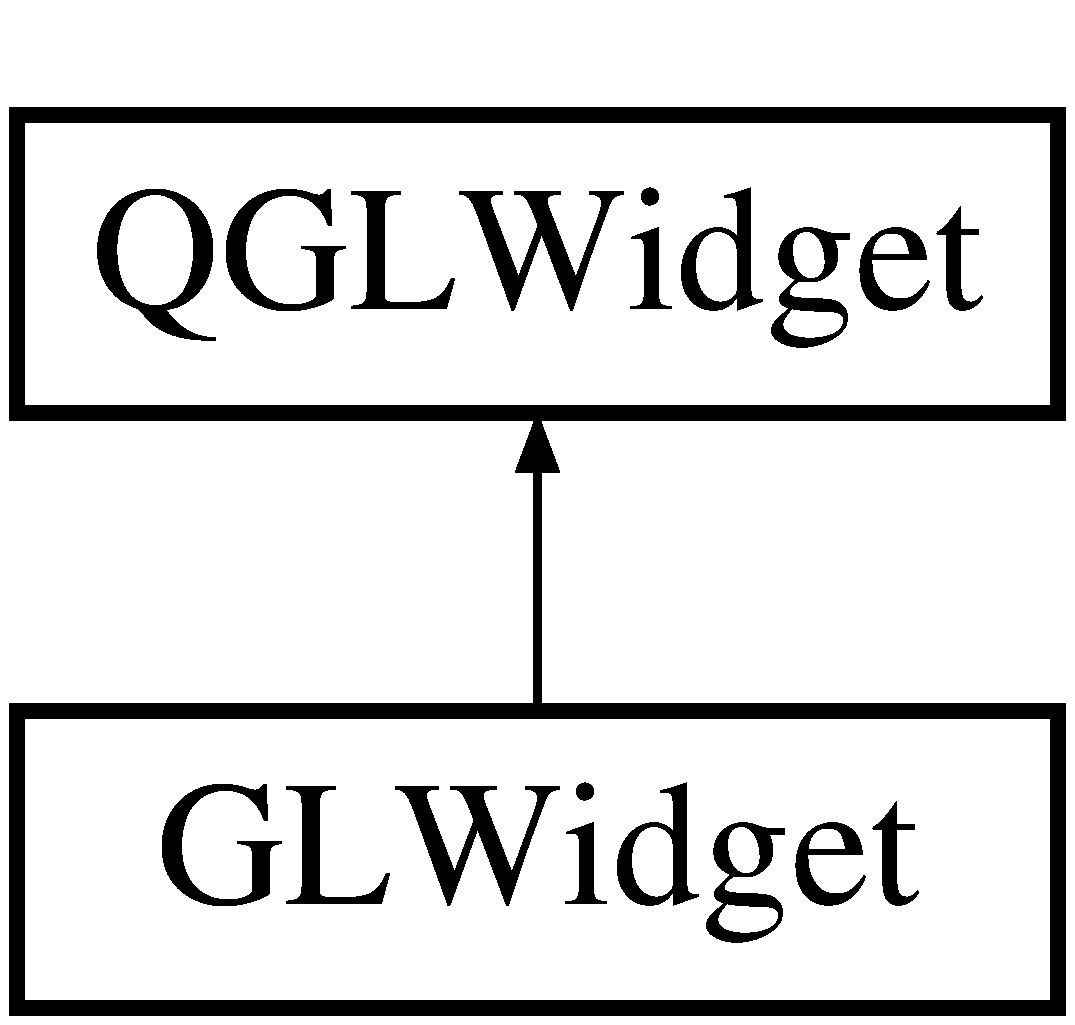
\includegraphics[height=2.000000cm]{classGLWidget}
\end{center}
\end{figure}
\subsection*{Signals}
\begin{DoxyCompactItemize}
\item 
\hypertarget{classGLWidget_a031d84e410b07e5c8afca4ab11e06c54}{}void {\bfseries Selected\+Item\+Changed} ()\label{classGLWidget_a031d84e410b07e5c8afca4ab11e06c54}

\item 
\hypertarget{classGLWidget_a628dd262f28dda97912e2f5d61eb8c6a}{}void {\bfseries Need\+To\+Clear\+Manual\+Element\+Selection} ()\label{classGLWidget_a628dd262f28dda97912e2f5d61eb8c6a}

\item 
\hypertarget{classGLWidget_a7bbc4801f4a079987dd5e7f46137b314}{}void {\bfseries Need\+To\+Clear\+Manual\+Node\+Selection} ()\label{classGLWidget_a7bbc4801f4a079987dd5e7f46137b314}

\end{DoxyCompactItemize}
\subsection*{Public Member Functions}
\begin{DoxyCompactItemize}
\item 
\hypertarget{classGLWidget_ab79c391c86de1ffb76f6950b49d82c0c}{}{\bfseries G\+L\+Widget} (Q\+Widget $\ast$parent=0)\label{classGLWidget_ab79c391c86de1ffb76f6950b49d82c0c}

\item 
\hypertarget{classGLWidget_ade3142625c1bfda0576e419b176cf8b1}{}Q\+Size {\bfseries minimum\+Size\+Hint} () const \label{classGLWidget_ade3142625c1bfda0576e419b176cf8b1}

\item 
\hypertarget{classGLWidget_a57698bc426052845b43a135a13540154}{}Q\+Size {\bfseries size\+Hint} () const \label{classGLWidget_a57698bc426052845b43a135a13540154}

\item 
\hypertarget{classGLWidget_ad425870ac081f6814c5bdb794e6e4c21}{}void {\bfseries manual\+Element\+Selection} (int i)\label{classGLWidget_ad425870ac081f6814c5bdb794e6e4c21}

\item 
\hypertarget{classGLWidget_a21f7a00a668f6ab6c5a9b1491e30c43e}{}void {\bfseries manual\+Node\+Selection} (int i)\label{classGLWidget_a21f7a00a668f6ab6c5a9b1491e30c43e}

\item 
\hypertarget{classGLWidget_ad569f9af7f5bbbfee5f1810d07107f20}{}void {\bfseries update\+Clipping} ()\label{classGLWidget_ad569f9af7f5bbbfee5f1810d07107f20}

\item 
\hypertarget{classGLWidget_adf09146230a2acda5a955acf59fbc653}{}void {\bfseries update\+To\+Top\+View} ()\label{classGLWidget_adf09146230a2acda5a955acf59fbc653}

\item 
\hypertarget{classGLWidget_ab4dcb3e931649a5f1edb6c6cede31075}{}void {\bfseries update\+To\+Front\+View} ()\label{classGLWidget_ab4dcb3e931649a5f1edb6c6cede31075}

\item 
\hypertarget{classGLWidget_a4930d77748cd175e349194da489c12d5}{}void {\bfseries update\+To\+Side\+View} ()\label{classGLWidget_a4930d77748cd175e349194da489c12d5}

\item 
\hypertarget{classGLWidget_afa3014a464a473c9ba62b22720f2d6fd}{}void {\bfseries update\+To\+Perspective\+View} ()\label{classGLWidget_afa3014a464a473c9ba62b22720f2d6fd}

\item 
\hypertarget{classGLWidget_af9b7537315485a04dd848ee62ac60b1e}{}void {\bfseries draw\+Points\+For\+Display} ()\label{classGLWidget_af9b7537315485a04dd848ee62ac60b1e}

\end{DoxyCompactItemize}
\subsection*{Public Attributes}
\begin{DoxyCompactItemize}
\item 
\hypertarget{classGLWidget_a9d11c25470e7e6d635d90b9605d54a2e}{}\hyperlink{classSimulation}{Simulation} $\ast$ {\bfseries Sim01}\label{classGLWidget_a9d11c25470e7e6d635d90b9605d54a2e}

\item 
\hypertarget{classGLWidget_a37fa0d9c8bfb720f550365da0aefccc7}{}bool {\bfseries Item\+Selected}\label{classGLWidget_a37fa0d9c8bfb720f550365da0aefccc7}

\item 
\hypertarget{classGLWidget_a67bf1bb7f19922f4ccb6728f339920e4}{}string {\bfseries Selected\+Item\+Name}\label{classGLWidget_a67bf1bb7f19922f4ccb6728f339920e4}

\item 
\hypertarget{classGLWidget_a908e8a53461c09eacf8d82d78d0a84d3}{}int {\bfseries Selected\+Item\+Index}\label{classGLWidget_a908e8a53461c09eacf8d82d78d0a84d3}

\item 
\hypertarget{classGLWidget_ab9d645f750345fde45fea123debb7f27}{}bool {\bfseries Manual\+Node\+Selection}\label{classGLWidget_ab9d645f750345fde45fea123debb7f27}

\item 
\hypertarget{classGLWidget_a4dac57a8924f1f9feb6d6bae75fe6d13}{}int {\bfseries Manual\+Selected\+Node\+Id}\label{classGLWidget_a4dac57a8924f1f9feb6d6bae75fe6d13}

\item 
\hypertarget{classGLWidget_a314984029a390e02a2d4235c5c2741a5}{}bool {\bfseries Display\+Strains}\label{classGLWidget_a314984029a390e02a2d4235c5c2741a5}

\item 
\hypertarget{classGLWidget_a753550713effac7b997844f2759c6129}{}float {\bfseries Display\+Strain\+Range} \mbox{[}2\mbox{]}\label{classGLWidget_a753550713effac7b997844f2759c6129}

\item 
\hypertarget{classGLWidget_ae95a720ff47f77ab05229d6502223c6f}{}int {\bfseries Strain\+To\+Display}\label{classGLWidget_ae95a720ff47f77ab05229d6502223c6f}

\item 
\hypertarget{classGLWidget_a9a990de1ec4c0e18778611cb0159eac8}{}bool {\bfseries Display\+Pys\+Prop}\label{classGLWidget_a9a990de1ec4c0e18778611cb0159eac8}

\item 
\hypertarget{classGLWidget_a478ab24d1ae3c646f40afedb72b725ae}{}int {\bfseries Pys\+Prop\+To\+Display}\label{classGLWidget_a478ab24d1ae3c646f40afedb72b725ae}

\item 
\hypertarget{classGLWidget_a04ab3aa5ad2078d0a495379907eb63ae}{}float {\bfseries Display\+Pys\+Prop\+Range} \mbox{[}6\mbox{]}\mbox{[}2\mbox{]}\label{classGLWidget_a04ab3aa5ad2078d0a495379907eb63ae}

\item 
\hypertarget{classGLWidget_a9bad9c8e609c86125850e2f83350d704}{}float {\bfseries Display\+Pys\+Prop\+Bounds} \mbox{[}6\mbox{]}\mbox{[}4\mbox{]}\label{classGLWidget_a9bad9c8e609c86125850e2f83350d704}

\item 
\hypertarget{classGLWidget_a93d20b91ca92dcd761870fb05291d9cd}{}int {\bfseries Display\+Pys\+Prop\+Decimals} \mbox{[}6\mbox{]}\label{classGLWidget_a93d20b91ca92dcd761870fb05291d9cd}

\item 
\hypertarget{classGLWidget_ae93978d9d5561027cf8697694ca695d3}{}float {\bfseries Display\+Pys\+Prop\+Steps} \mbox{[}6\mbox{]}\label{classGLWidget_ae93978d9d5561027cf8697694ca695d3}

\item 
\hypertarget{classGLWidget_ac238abe591ebaf2aa26a65378a65ce0f}{}vector$<$ Q\+String $>$ {\bfseries Selected\+Pos}\label{classGLWidget_ac238abe591ebaf2aa26a65378a65ce0f}

\item 
\hypertarget{classGLWidget_a358fbf9622862b7fd18a5eafca90aaf2}{}vector$<$ Q\+String $>$ {\bfseries Selected\+Id}\label{classGLWidget_a358fbf9622862b7fd18a5eafca90aaf2}

\item 
\hypertarget{classGLWidget_a66ce8db8191fcb7bac6e7d819bb30b95}{}bool {\bfseries draw\+Net\+Forces}\label{classGLWidget_a66ce8db8191fcb7bac6e7d819bb30b95}

\item 
\hypertarget{classGLWidget_a993ff9e84e7837735b14743a10cd6ddd}{}bool {\bfseries draw\+Myosin\+Forces}\label{classGLWidget_a993ff9e84e7837735b14743a10cd6ddd}

\item 
\hypertarget{classGLWidget_ab9f882d19b598a85dc5da6201681376a}{}int {\bfseries Myosin\+To\+Display}\label{classGLWidget_ab9f882d19b598a85dc5da6201681376a}

\item 
\hypertarget{classGLWidget_a667580ff60b536f89e8b693c6f043868}{}bool {\bfseries draw\+Packing\+Forces}\label{classGLWidget_a667580ff60b536f89e8b693c6f043868}

\item 
\hypertarget{classGLWidget_ae57adc8b63690ebf5bf1d3e4ab35ae44}{}bool {\bfseries draw\+Velocities}\label{classGLWidget_ae57adc8b63690ebf5bf1d3e4ab35ae44}

\item 
\hypertarget{classGLWidget_a1198d8100d85dec3c9a106081d1465df}{}bool {\bfseries draw\+Tissue\+Scale\+Bar}\label{classGLWidget_a1198d8100d85dec3c9a106081d1465df}

\item 
\hypertarget{classGLWidget_af59fc963b9eaf559dfd0ad41cf88dac0}{}bool {\bfseries draw\+Peripodial\+Membrane}\label{classGLWidget_af59fc963b9eaf559dfd0ad41cf88dac0}

\item 
\hypertarget{classGLWidget_a404f4d4130a0c3ea84aeaaac6adb618b}{}bool {\bfseries draw\+Columnar}\label{classGLWidget_a404f4d4130a0c3ea84aeaaac6adb618b}

\item 
\hypertarget{classGLWidget_ac011fc6341a41ec96b9a2a332e223617}{}bool {\bfseries Perspective\+View}\label{classGLWidget_ac011fc6341a41ec96b9a2a332e223617}

\item 
\hypertarget{classGLWidget_a2f10bf15fc043faacc7aa533ca31c3ee}{}bool {\bfseries display\+Bounding\+Box}\label{classGLWidget_a2f10bf15fc043faacc7aa533ca31c3ee}

\item 
\hypertarget{classGLWidget_a16bec7573f51d68f7606c13d258fdff2}{}bool {\bfseries display\+Pipette}\label{classGLWidget_a16bec7573f51d68f7606c13d258fdff2}

\item 
\hypertarget{classGLWidget_a24d8815d6f656844dabf893a09bee5d6}{}double {\bfseries x\+Clip}\label{classGLWidget_a24d8815d6f656844dabf893a09bee5d6}

\item 
\hypertarget{classGLWidget_a688447afa71d6b4b004a933991f2d8de}{}double {\bfseries y\+Clip}\label{classGLWidget_a688447afa71d6b4b004a933991f2d8de}

\item 
\hypertarget{classGLWidget_a3deec68705f88f3d1653b380f8c918b3}{}double {\bfseries z\+Clip}\label{classGLWidget_a3deec68705f88f3d1653b380f8c918b3}

\item 
\hypertarget{classGLWidget_a50707fe8f3eb2f48a541094af67c0e2b}{}bool {\bfseries draw\+Symmetricity}\label{classGLWidget_a50707fe8f3eb2f48a541094af67c0e2b}

\end{DoxyCompactItemize}
\subsection*{Protected Member Functions}
\begin{DoxyCompactItemize}
\item 
\hypertarget{classGLWidget_a7fab13e8cc9fc0730ca54c08b2c923a7}{}void {\bfseries initialize\+G\+L} ()\label{classGLWidget_a7fab13e8cc9fc0730ca54c08b2c923a7}

\item 
\hypertarget{classGLWidget_a640b5570cb2b37724fd5b58a77339c5e}{}void {\bfseries paint\+G\+L} ()\label{classGLWidget_a640b5570cb2b37724fd5b58a77339c5e}

\item 
\hypertarget{classGLWidget_ac0d2a8ecf60907a81c0d73475d851025}{}void {\bfseries resize\+G\+L} (int width, int height)\label{classGLWidget_ac0d2a8ecf60907a81c0d73475d851025}

\item 
\hypertarget{classGLWidget_ab144cc8064c1bbf6d0ef0646ca0bd06c}{}void {\bfseries mouse\+Press\+Event} (Q\+Mouse\+Event $\ast$event)\label{classGLWidget_ab144cc8064c1bbf6d0ef0646ca0bd06c}

\item 
\hypertarget{classGLWidget_ab992c4c25439a5ef23031991015451c1}{}void {\bfseries mouse\+Release\+Event} (Q\+Mouse\+Event $\ast$event)\label{classGLWidget_ab992c4c25439a5ef23031991015451c1}

\item 
\hypertarget{classGLWidget_a9043bac13d6f0a5307ea5c7f9b3caa50}{}void {\bfseries mouse\+Move\+Event} (Q\+Mouse\+Event $\ast$event)\label{classGLWidget_a9043bac13d6f0a5307ea5c7f9b3caa50}

\item 
\hypertarget{classGLWidget_a5702a23f7cf42d05fe55a417d810a4b6}{}void {\bfseries wheel\+Event} (Q\+Wheel\+Event $\ast$event)\label{classGLWidget_a5702a23f7cf42d05fe55a417d810a4b6}

\item 
\hypertarget{classGLWidget_af102973086f831f0a27b3458c57bb337}{}void {\bfseries Object\+Selection} (Q\+Point Last\+Pos)\label{classGLWidget_af102973086f831f0a27b3458c57bb337}

\item 
\hypertarget{classGLWidget_a4aba027a507e84b880acd641275165d4}{}void {\bfseries reset\+Item\+Selection\+Info} (int source)\label{classGLWidget_a4aba027a507e84b880acd641275165d4}

\item 
\hypertarget{classGLWidget_a7fe217738ad7d4c54caa575068641234}{}void {\bfseries find\+Element} ()\label{classGLWidget_a7fe217738ad7d4c54caa575068641234}

\item 
\hypertarget{classGLWidget_aa1c349f897d0fee1163abba8fd39995c}{}bool {\bfseries find\+Element} (int i)\label{classGLWidget_aa1c349f897d0fee1163abba8fd39995c}

\item 
\hypertarget{classGLWidget_a7ff762be5c3562616b6cc4bc6d6b6683}{}bool {\bfseries find\+Node} (int i)\label{classGLWidget_a7ff762be5c3562616b6cc4bc6d6b6683}

\item 
\hypertarget{classGLWidget_afc09ab8fa7a8163ca1b69e7953e33dc4}{}void {\bfseries get\+Colour\+Of\+Point} (Q\+Point Last\+Pos)\label{classGLWidget_afc09ab8fa7a8163ca1b69e7953e33dc4}

\item 
\hypertarget{classGLWidget_a218fadfeda519fd8a120b702f04771c8}{}void {\bfseries draw\+For\+Picking} ()\label{classGLWidget_a218fadfeda519fd8a120b702f04771c8}

\item 
\hypertarget{classGLWidget_a1f66af8462807ed77b878cba3e60bbb9}{}void {\bfseries generate3\+D\+Object} ()\label{classGLWidget_a1f66af8462807ed77b878cba3e60bbb9}

\item 
\hypertarget{classGLWidget_a30be9e529d717552be70cbad097d99e8}{}void {\bfseries initialise\+Node\+Colour\+List} ()\label{classGLWidget_a30be9e529d717552be70cbad097d99e8}

\item 
\hypertarget{classGLWidget_a8597de4600272fb1720641fd1990f153}{}bool {\bfseries check\+If\+Drawing\+Element} (int i)\label{classGLWidget_a8597de4600272fb1720641fd1990f153}

\item 
\hypertarget{classGLWidget_a95a5dc2578aeaf9df7127c0af7d1a531}{}bool {\bfseries check\+If\+Drawing\+Element\+Symmetric} (int i, bool symmetric\+X, bool symmetric\+Y)\label{classGLWidget_a95a5dc2578aeaf9df7127c0af7d1a531}

\item 
\hypertarget{classGLWidget_a4e843eda050d818414f6c722f806cf88}{}bool {\bfseries check\+If\+Drawing\+Node} (int i)\label{classGLWidget_a4e843eda050d818414f6c722f806cf88}

\item 
\hypertarget{classGLWidget_aa85fc1e14fb11fc62ce93cc72ffb5a61}{}void {\bfseries draw\+Element} (int i, bool picking)\label{classGLWidget_aa85fc1e14fb11fc62ce93cc72ffb5a61}

\item 
\hypertarget{classGLWidget_ada0503af64f483c91e342ba5c3dcef49}{}void {\bfseries highlight\+Element} (int i)\label{classGLWidget_ada0503af64f483c91e342ba5c3dcef49}

\item 
\hypertarget{classGLWidget_addb75eed990f0b943d47009f14e8a3de}{}void {\bfseries highlight\+Node} (int i)\label{classGLWidget_addb75eed990f0b943d47009f14e8a3de}

\item 
\hypertarget{classGLWidget_a7be96b028f099e61dfbc75254316c078}{}void {\bfseries draw\+Reference\+Element} (int i)\label{classGLWidget_a7be96b028f099e61dfbc75254316c078}

\item 
\hypertarget{classGLWidget_a523f68e2bf91f762bbd4fb5ab734e737}{}void {\bfseries draw\+Prism} (int i, bool symmetric\+X, bool symmetric\+Y)\label{classGLWidget_a523f68e2bf91f762bbd4fb5ab734e737}

\item 
\hypertarget{classGLWidget_a61c80b66b9686c4325dec480f6d3eef9}{}void {\bfseries draw\+Triangle} (int i)\label{classGLWidget_a61c80b66b9686c4325dec480f6d3eef9}

\item 
\hypertarget{classGLWidget_a36c00f9f2aec8eff1291efd1416be16e}{}void {\bfseries draw\+Prism\+For\+Picking} (int i)\label{classGLWidget_a36c00f9f2aec8eff1291efd1416be16e}

\item 
\hypertarget{classGLWidget_a1b670bed499c7bb756cae4b7b2153426}{}void {\bfseries draw\+Triangle\+For\+Picking} (int i)\label{classGLWidget_a1b670bed499c7bb756cae4b7b2153426}

\item 
\hypertarget{classGLWidget_aae1cc6d1837d0d0bb454eb0dda4b5a7c}{}void {\bfseries draw\+Reference\+Prism} (int i)\label{classGLWidget_aae1cc6d1837d0d0bb454eb0dda4b5a7c}

\item 
\hypertarget{classGLWidget_a80bd480b4e4828e7cc6e043805f804ac}{}void {\bfseries draw\+Reference\+Triangle} (int i)\label{classGLWidget_a80bd480b4e4828e7cc6e043805f804ac}

\item 
\hypertarget{classGLWidget_a3486092418bb1d3050860c7b4539fef1}{}void {\bfseries highlight\+Prism} (int i)\label{classGLWidget_a3486092418bb1d3050860c7b4539fef1}

\item 
\hypertarget{classGLWidget_aa3bfac7b767b04f2dd0685692b4f5aa2}{}void {\bfseries highlight\+Triangle} (int i)\label{classGLWidget_aa3bfac7b767b04f2dd0685692b4f5aa2}

\item 
\hypertarget{classGLWidget_af2ce64f5342b0a42f9460a9173b7eaf7}{}void {\bfseries fill\+Item\+Selection\+Info} (int i)\label{classGLWidget_af2ce64f5342b0a42f9460a9173b7eaf7}

\end{DoxyCompactItemize}


\subsection{Detailed Description}
\hyperlink{classGLWidget}{G\+L\+Widget} class 

The documentation for this class was generated from the following files\+:\begin{DoxyCompactItemize}
\item 
/home/melda/\+Documents/\+Tissue\+Folding/\+User\+Interface/\+Source\+Code/G\+L\+Widget.\+h\item 
/home/melda/\+Documents/\+Tissue\+Folding/\+User\+Interface/\+Source\+Code/G\+L\+Widget.\+cpp\end{DoxyCompactItemize}

\hypertarget{classGridBasedGrowthFunction}{}\section{Grid\+Based\+Growth\+Function Class Reference}
\label{classGridBasedGrowthFunction}\index{Grid\+Based\+Growth\+Function@{Grid\+Based\+Growth\+Function}}
Inheritance diagram for Grid\+Based\+Growth\+Function\+:\begin{figure}[H]
\begin{center}
\leavevmode
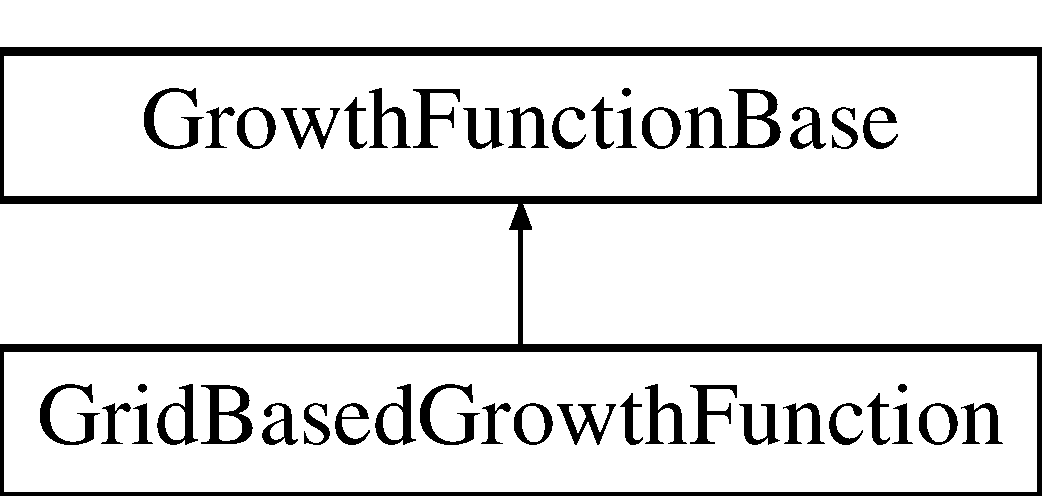
\includegraphics[height=2.000000cm]{classGridBasedGrowthFunction}
\end{center}
\end{figure}
\subsection*{Public Member Functions}
\begin{DoxyCompactItemize}
\item 
\hyperlink{classGridBasedGrowthFunction_aac341fa9ccdca2d089e9f341cb68ca94}{Grid\+Based\+Growth\+Function} (int id, int type, float \hyperlink{classGrowthFunctionBase_ae92513a7b41637df8e26e7db35ddf97c}{init\+Time}, float \hyperlink{classGrowthFunctionBase_a3ff4db0573d354a75666a5f3ca446941}{end\+Time}, bool \hyperlink{classGrowthFunctionBase_a3d56771e7c145589a14e11cc331e0326}{apply\+To\+Columnar\+Layer}, bool \hyperlink{classGrowthFunctionBase_a08ae19f58cb98fa8e315a77f52749732}{apply\+To\+Peripodial\+Membrane}, int n\+X, int n\+Y, double $\ast$$\ast$$\ast$Growth\+Mat, double $\ast$$\ast$Angle\+Mat)
\begin{DoxyCompactList}\small\item\em The constructor of \hyperlink{classGridBasedGrowthFunction}{Grid\+Based\+Growth\+Function}. \end{DoxyCompactList}\item 
\hypertarget{classGridBasedGrowthFunction_ae36e6ea2e7bdf41459e74d5846d6d24d}{}int \hyperlink{classGridBasedGrowthFunction_ae36e6ea2e7bdf41459e74d5846d6d24d}{get\+Grid\+X} ()\label{classGridBasedGrowthFunction_ae36e6ea2e7bdf41459e74d5846d6d24d}

\begin{DoxyCompactList}\small\item\em This function returns \hyperlink{classGridBasedGrowthFunction_af872b9963f3a579dcd615c23bcb58a86}{Grid\+Based\+Growth\+Function\+::n\+Grid\+X}. \end{DoxyCompactList}\item 
\hypertarget{classGridBasedGrowthFunction_a4a70e9e187e3079e29115f106d30e26e}{}int \hyperlink{classGridBasedGrowthFunction_a4a70e9e187e3079e29115f106d30e26e}{get\+Grid\+Y} ()\label{classGridBasedGrowthFunction_a4a70e9e187e3079e29115f106d30e26e}

\begin{DoxyCompactList}\small\item\em This function returns \hyperlink{classGridBasedGrowthFunction_a625bc963a1f1e7d1f1a35dbd0ef51728}{Grid\+Based\+Growth\+Function\+::n\+Grid\+Y}. \end{DoxyCompactList}\item 
\hypertarget{classGridBasedGrowthFunction_ac25ac1f12b74816a1d3d3e5dda0e8541}{}double $\ast$$\ast$$\ast$ \hyperlink{classGridBasedGrowthFunction_ac25ac1f12b74816a1d3d3e5dda0e8541}{get\+Growth\+Matrix} ()\label{classGridBasedGrowthFunction_ac25ac1f12b74816a1d3d3e5dda0e8541}

\begin{DoxyCompactList}\small\item\em This function returns \hyperlink{classGridBasedGrowthFunction_a5522d9b84fa95ebd65cdf290a4f0a65c}{Grid\+Based\+Growth\+Function\+::\+Growth\+Matrix}. \end{DoxyCompactList}\item 
\hypertarget{classGridBasedGrowthFunction_ad590b4a5c6e5e47f5679de5a8c6cb738}{}double $\ast$$\ast$ \hyperlink{classGridBasedGrowthFunction_ad590b4a5c6e5e47f5679de5a8c6cb738}{get\+Xy\+Shear\+Angle\+Matrix} ()\label{classGridBasedGrowthFunction_ad590b4a5c6e5e47f5679de5a8c6cb738}

\begin{DoxyCompactList}\small\item\em This function returns \hyperlink{classGridBasedGrowthFunction_aa01cee8282299e18f27b47645da17438}{Grid\+Based\+Growth\+Function\+::xy\+Shear\+Angle\+Matrix}. \end{DoxyCompactList}\item 
\hypertarget{classGridBasedGrowthFunction_a1775fe1788bc97569c892d01cc625ea8}{}double \hyperlink{classGridBasedGrowthFunction_a1775fe1788bc97569c892d01cc625ea8}{get\+Growth\+Matrix\+Element} (int i, int j, int k)\label{classGridBasedGrowthFunction_a1775fe1788bc97569c892d01cc625ea8}

\begin{DoxyCompactList}\small\item\em This function returns the growth rate at grid point \mbox{[}i\mbox{]}\mbox{[}j\mbox{]} (in dimensions \hyperlink{classGridBasedGrowthFunction_af872b9963f3a579dcd615c23bcb58a86}{Grid\+Based\+Growth\+Function\+::n\+Grid\+X}, \hyperlink{classGridBasedGrowthFunction_a625bc963a1f1e7d1f1a35dbd0ef51728}{Grid\+Based\+Growth\+Function\+::n\+Grid\+Y}), for the growth dimension \mbox{[}k\mbox{]} (as in \mbox{[} D\+V axis (x), A\+P axis (y), and A\+B axis (z)\mbox{]} ). \end{DoxyCompactList}\item 
\hypertarget{classGridBasedGrowthFunction_a5075a53329b3a0b73a5864b7ffb37c5d}{}double \hyperlink{classGridBasedGrowthFunction_a5075a53329b3a0b73a5864b7ffb37c5d}{get\+Xy\+Shear\+Angle\+Matrix\+Element} (int i, int j)\label{classGridBasedGrowthFunction_a5075a53329b3a0b73a5864b7ffb37c5d}

\begin{DoxyCompactList}\small\item\em This function returns the xy\+Shear angle at grid point \mbox{[}i\mbox{]}\mbox{[}j\mbox{]} (in dimensions \hyperlink{classGridBasedGrowthFunction_af872b9963f3a579dcd615c23bcb58a86}{Grid\+Based\+Growth\+Function\+::n\+Grid\+X}, \hyperlink{classGridBasedGrowthFunction_a625bc963a1f1e7d1f1a35dbd0ef51728}{Grid\+Based\+Growth\+Function\+::n\+Grid\+Y}). \end{DoxyCompactList}\item 
\hypertarget{classGridBasedGrowthFunction_a85ed4f6a4b5165adf1ab8806b885f81a}{}gsl\+\_\+matrix $\ast$ \hyperlink{classGridBasedGrowthFunction_a85ed4f6a4b5165adf1ab8806b885f81a}{get\+Xy\+Shear\+Rotations\+Matrix\+Element} (int i, int j)\label{classGridBasedGrowthFunction_a85ed4f6a4b5165adf1ab8806b885f81a}

\begin{DoxyCompactList}\small\item\em This function returns the xy\+Shear rotation matrix at grid point \mbox{[}i\mbox{]}\mbox{[}j\mbox{]} (in dimensions \hyperlink{classGridBasedGrowthFunction_af872b9963f3a579dcd615c23bcb58a86}{Grid\+Based\+Growth\+Function\+::n\+Grid\+X}, \hyperlink{classGridBasedGrowthFunction_a625bc963a1f1e7d1f1a35dbd0ef51728}{Grid\+Based\+Growth\+Function\+::n\+Grid\+Y}). \end{DoxyCompactList}\item 
\hypertarget{classGridBasedGrowthFunction_ab07937a18f72f31f4875225c1e246032}{}bool {\bfseries is\+Aspect\+Ratio\+Over\+One} (int i, int j)\label{classGridBasedGrowthFunction_ab07937a18f72f31f4875225c1e246032}

\item 
\hypertarget{classGridBasedGrowthFunction_a9d01fcbba5732aad966659d4f64c145b}{}void \hyperlink{classGridBasedGrowthFunction_a9d01fcbba5732aad966659d4f64c145b}{set\+Growth\+Matrix\+Element} (double ex, double ey, double ez, int i, int j)\label{classGridBasedGrowthFunction_a9d01fcbba5732aad966659d4f64c145b}

\begin{DoxyCompactList}\small\item\em This function sets the growth rate at grid point \mbox{[}i\mbox{]}\mbox{[}j\mbox{]} (in dimensions \hyperlink{classGridBasedGrowthFunction_af872b9963f3a579dcd615c23bcb58a86}{Grid\+Based\+Growth\+Function\+::n\+Grid\+X}, \hyperlink{classGridBasedGrowthFunction_a625bc963a1f1e7d1f1a35dbd0ef51728}{Grid\+Based\+Growth\+Function\+::n\+Grid\+Y}), to the growth rate \mbox{[}ex, ey, ez\mbox{]} in the format \mbox{[} D\+V axis (x), A\+P axis (y), and A\+B axis (z)\mbox{]}. \end{DoxyCompactList}\item 
\hypertarget{classGridBasedGrowthFunction_a92f4db6ab17ba3539f98895c500ec2d7}{}void {\bfseries pre\+Calculate\+Angles\+For\+Compatible\+Averaging} ()\label{classGridBasedGrowthFunction_a92f4db6ab17ba3539f98895c500ec2d7}

\item 
\hypertarget{classGridBasedGrowthFunction_a11692e47b20e812fe775f99a78480571}{}void {\bfseries get\+Growth\+Profile\+At4\+Corners} (int Index\+X, int Index\+Y, double $\ast$growth0, double $\ast$growth1, double $\ast$growth2, double $\ast$growth3, double $\ast$angles, bool $\ast$angles\+Eliminated)\label{classGridBasedGrowthFunction_a11692e47b20e812fe775f99a78480571}

\item 
void \hyperlink{classGridBasedGrowthFunction_a659418841b4a3bc8be1dec15f95d7b76}{write\+Summary} (ofstream \&save\+File\+Simulation\+Summary, double dt)
\begin{DoxyCompactList}\small\item\em The function is to write the growth function summary to simulation summary file. \end{DoxyCompactList}\end{DoxyCompactItemize}
\subsection*{Public Attributes}
\begin{DoxyCompactItemize}
\item 
\hypertarget{classGridBasedGrowthFunction_af872b9963f3a579dcd615c23bcb58a86}{}int \hyperlink{classGridBasedGrowthFunction_af872b9963f3a579dcd615c23bcb58a86}{n\+Grid\+X}\label{classGridBasedGrowthFunction_af872b9963f3a579dcd615c23bcb58a86}

\begin{DoxyCompactList}\small\item\em The number of grid points that discretise the tissue in x. \end{DoxyCompactList}\item 
\hypertarget{classGridBasedGrowthFunction_a625bc963a1f1e7d1f1a35dbd0ef51728}{}int \hyperlink{classGridBasedGrowthFunction_a625bc963a1f1e7d1f1a35dbd0ef51728}{n\+Grid\+Y}\label{classGridBasedGrowthFunction_a625bc963a1f1e7d1f1a35dbd0ef51728}

\begin{DoxyCompactList}\small\item\em The number of grid points that discretise the tissue in y. \end{DoxyCompactList}\item 
\hypertarget{classGridBasedGrowthFunction_a5522d9b84fa95ebd65cdf290a4f0a65c}{}double $\ast$$\ast$$\ast$ \hyperlink{classGridBasedGrowthFunction_a5522d9b84fa95ebd65cdf290a4f0a65c}{Growth\+Matrix}\label{classGridBasedGrowthFunction_a5522d9b84fa95ebd65cdf290a4f0a65c}

\begin{DoxyCompactList}\small\item\em The matrix of growth rates in (1/sec). It is a matrix of double triplets for growth rate at each grid point. The dimensions of the matrix are equal to (\hyperlink{classGridBasedGrowthFunction_af872b9963f3a579dcd615c23bcb58a86}{Grid\+Based\+Growth\+Function\+::n\+Grid\+X}, \hyperlink{classGridBasedGrowthFunction_a625bc963a1f1e7d1f1a35dbd0ef51728}{Grid\+Based\+Growth\+Function\+::n\+Grid\+Y}), and set in constructor of the \hyperlink{classGridBasedGrowthFunction}{Grid\+Based\+Growth\+Function}. The triplets store the growth rate in \mbox{[} D\+V axis (x), A\+P axis (y), and A\+B axis (z)\mbox{]}. \end{DoxyCompactList}\item 
\hypertarget{classGridBasedGrowthFunction_aa01cee8282299e18f27b47645da17438}{}double $\ast$$\ast$ \hyperlink{classGridBasedGrowthFunction_aa01cee8282299e18f27b47645da17438}{xy\+Shear\+Angle\+Matrix}\label{classGridBasedGrowthFunction_aa01cee8282299e18f27b47645da17438}

\begin{DoxyCompactList}\small\item\em The matrix of xy shear rate (rad/sec). It is a matrix of doubles at each grid point. he dimensions of the matrix are equal to (\hyperlink{classGridBasedGrowthFunction_af872b9963f3a579dcd615c23bcb58a86}{Grid\+Based\+Growth\+Function\+::n\+Grid\+X}, \hyperlink{classGridBasedGrowthFunction_a625bc963a1f1e7d1f1a35dbd0ef51728}{Grid\+Based\+Growth\+Function\+::n\+Grid\+Y}), and set in constructor of the \hyperlink{classGridBasedGrowthFunction}{Grid\+Based\+Growth\+Function}. \end{DoxyCompactList}\item 
\hypertarget{classGridBasedGrowthFunction_a62e3267b367261ff2f37cee9a7c2b02b}{}gsl\+\_\+matrix $\ast$$\ast$$\ast$ {\bfseries xy\+Shear\+Rotations\+Matrix}\label{classGridBasedGrowthFunction_a62e3267b367261ff2f37cee9a7c2b02b}

\item 
\hypertarget{classGridBasedGrowthFunction_a56ff4380487e4d24881431f0e6ea6f2e}{}bool $\ast$$\ast$ {\bfseries aspect\+Ratio\+Over\+Thresold\+Matrix}\label{classGridBasedGrowthFunction_a56ff4380487e4d24881431f0e6ea6f2e}

\item 
\hypertarget{classGridBasedGrowthFunction_a59b0e127387157f89f099ae3beeaa671}{}double $\ast$$\ast$$\ast$$\ast$ {\bfseries compatible\+Growths}\label{classGridBasedGrowthFunction_a59b0e127387157f89f099ae3beeaa671}

\item 
\hypertarget{classGridBasedGrowthFunction_aac8a163bbd008d327859b488cf023c10}{}double $\ast$$\ast$$\ast$ {\bfseries compatible\+Angles}\label{classGridBasedGrowthFunction_aac8a163bbd008d327859b488cf023c10}

\item 
\hypertarget{classGridBasedGrowthFunction_addfc2d280d1fc0b0b17d7f1dfe54f873}{}bool $\ast$$\ast$$\ast$ {\bfseries compatible\+Angle\+Eliminated}\label{classGridBasedGrowthFunction_addfc2d280d1fc0b0b17d7f1dfe54f873}

\end{DoxyCompactItemize}


\subsection{Constructor \& Destructor Documentation}
\hypertarget{classGridBasedGrowthFunction_aac341fa9ccdca2d089e9f341cb68ca94}{}\index{Grid\+Based\+Growth\+Function@{Grid\+Based\+Growth\+Function}!Grid\+Based\+Growth\+Function@{Grid\+Based\+Growth\+Function}}
\index{Grid\+Based\+Growth\+Function@{Grid\+Based\+Growth\+Function}!Grid\+Based\+Growth\+Function@{Grid\+Based\+Growth\+Function}}
\subsubsection[{Grid\+Based\+Growth\+Function}]{\setlength{\rightskip}{0pt plus 5cm}Grid\+Based\+Growth\+Function\+::\+Grid\+Based\+Growth\+Function (
\begin{DoxyParamCaption}
\item[{int}]{id, }
\item[{int}]{type, }
\item[{float}]{init\+Time, }
\item[{float}]{end\+Time, }
\item[{bool}]{apply\+To\+Columnar\+Layer, }
\item[{bool}]{apply\+To\+Peripodial\+Membrane, }
\item[{int}]{n\+X, }
\item[{int}]{n\+Y, }
\item[{double $\ast$$\ast$$\ast$}]{Growth\+Mat, }
\item[{double $\ast$$\ast$}]{Angle\+Mat}
\end{DoxyParamCaption}
)\hspace{0.3cm}{\ttfamily [inline]}}\label{classGridBasedGrowthFunction_aac341fa9ccdca2d089e9f341cb68ca94}


The constructor of \hyperlink{classGridBasedGrowthFunction}{Grid\+Based\+Growth\+Function}. 

The first six parameters will be directed to the parent constructor, \hyperlink{classGrowthFunctionBase_a061b31ad8a0cb228628c7104029a94bf}{Growth\+Function\+Base\+::\+Growth\+Function\+Base}. ~\newline
integers n\+X and n\+Y will set \hyperlink{classGridBasedGrowthFunction_af872b9963f3a579dcd615c23bcb58a86}{Grid\+Based\+Growth\+Function\+::n\+Grid\+X} and \hyperlink{classGridBasedGrowthFunction_a625bc963a1f1e7d1f1a35dbd0ef51728}{Grid\+Based\+Growth\+Function\+::n\+Grid\+Y}, respectively. \hyperlink{classGridBasedGrowthFunction_a5522d9b84fa95ebd65cdf290a4f0a65c}{Grid\+Based\+Growth\+Function\+::\+Growth\+Matrix} will be initiated to point at a 2 dimensional matrix of double triplets the size(n\+X, n\+Y). ~\newline
double$\ast$$\ast$$\ast$ Growth\+Mat is the pointer to the 2-\/dimensional matrix of double triplets, holding the 3\+D growth rates at each grid point. Values stored in Growth\+Mat will set the values in \hyperlink{classGridBasedGrowthFunction_a5522d9b84fa95ebd65cdf290a4f0a65c}{Grid\+Based\+Growth\+Function\+::\+Growth\+Matrix}. The matrix storing the growth rates have been read from an input file through Model\+Input\+Object\+::read\+Growth\+Options and related functions therein ~\newline
 

\subsection{Member Function Documentation}
\hypertarget{classGridBasedGrowthFunction_a659418841b4a3bc8be1dec15f95d7b76}{}\index{Grid\+Based\+Growth\+Function@{Grid\+Based\+Growth\+Function}!write\+Summary@{write\+Summary}}
\index{write\+Summary@{write\+Summary}!Grid\+Based\+Growth\+Function@{Grid\+Based\+Growth\+Function}}
\subsubsection[{write\+Summary}]{\setlength{\rightskip}{0pt plus 5cm}void Grid\+Based\+Growth\+Function\+::write\+Summary (
\begin{DoxyParamCaption}
\item[{ofstream \&}]{save\+File\+Simulation\+Summary, }
\item[{double}]{dt}
\end{DoxyParamCaption}
)\hspace{0.3cm}{\ttfamily [inline]}, {\ttfamily [virtual]}}\label{classGridBasedGrowthFunction_a659418841b4a3bc8be1dec15f95d7b76}


The function is to write the growth function summary to simulation summary file. 

This function will write the \hyperlink{classGridBasedGrowthFunction}{Grid\+Based\+Growth\+Function} details into the simulation summary file, provided as the first input. Time step (dt) of the simulation is provided as second input, to report the growth rates per hour. The output should look like\+: ~\newline
 Growth Type\+: growth From File (3) Initial time(sec)\+: \hyperlink{classGrowthFunctionBase_ae92513a7b41637df8e26e7db35ddf97c}{Grid\+Based\+Growth\+Function\+::init\+Time} Final\+Time time(sec)\+: \hyperlink{classGrowthFunctionBase_a3ff4db0573d354a75666a5f3ca446941}{Grid\+Based\+Growth\+Function\+::end\+Time} Growth matrix mesh size\+: \hyperlink{classGridBasedGrowthFunction_af872b9963f3a579dcd615c23bcb58a86}{Grid\+Based\+Growth\+Function\+::n\+Grid\+X} \hyperlink{classGridBasedGrowthFunction_a625bc963a1f1e7d1f1a35dbd0ef51728}{Grid\+Based\+Growth\+Function\+::n\+Grid\+Y}

Reimplemented from \hyperlink{classGrowthFunctionBase}{Growth\+Function\+Base}.



The documentation for this class was generated from the following file\+:\begin{DoxyCompactItemize}
\item 
/home/melda/\+Documents/\+Tissue\+Folding/\+Tissue\+Folding/\+Source\+Code/Growth\+Function\+Types.\+h\end{DoxyCompactItemize}

\hypertarget{classGrowthFunctionBase}{}\section{Growth\+Function\+Base Class Reference}
\label{classGrowthFunctionBase}\index{Growth\+Function\+Base@{Growth\+Function\+Base}}
Inheritance diagram for Growth\+Function\+Base\+:\begin{figure}[H]
\begin{center}
\leavevmode
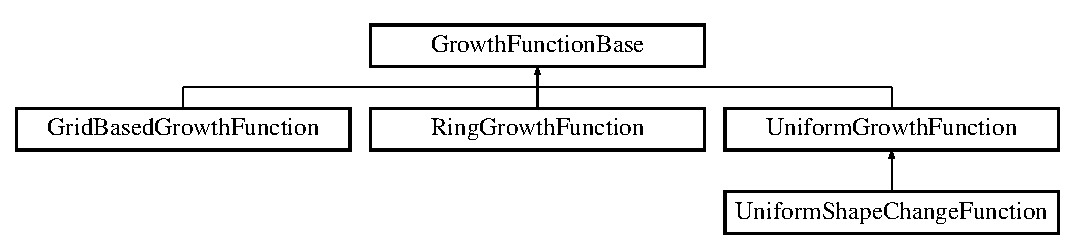
\includegraphics[height=2.916667cm]{classGrowthFunctionBase}
\end{center}
\end{figure}
\subsection*{Public Member Functions}
\begin{DoxyCompactItemize}
\item 
\hyperlink{classGrowthFunctionBase_a061b31ad8a0cb228628c7104029a94bf}{Growth\+Function\+Base} (int id, int type, float \hyperlink{classGrowthFunctionBase_ae92513a7b41637df8e26e7db35ddf97c}{init\+Time}, float \hyperlink{classGrowthFunctionBase_a3ff4db0573d354a75666a5f3ca446941}{end\+Time}, bool \hyperlink{classGrowthFunctionBase_a3d56771e7c145589a14e11cc331e0326}{apply\+To\+Columnar\+Layer}, bool \hyperlink{classGrowthFunctionBase_a08ae19f58cb98fa8e315a77f52749732}{apply\+To\+Peripodial\+Membrane})
\begin{DoxyCompactList}\small\item\em The constructor of \hyperlink{classGrowthFunctionBase}{Growth\+Function\+Base}. Different growth functions will be derived from this class. \end{DoxyCompactList}\item 
\hypertarget{classGrowthFunctionBase_ad5b4e88d33c4b72444c5c25c25ab68fb}{}void {\bfseries Parent\+Error\+Message} (string function\+Name)\label{classGrowthFunctionBase_ad5b4e88d33c4b72444c5c25c25ab68fb}

\item 
\hypertarget{classGrowthFunctionBase_aed234af9feb797628d4a2d598dcf9632}{}double {\bfseries Parent\+Error\+Message} (string function\+Name, double return\+Value)\label{classGrowthFunctionBase_aed234af9feb797628d4a2d598dcf9632}

\item 
\hypertarget{classGrowthFunctionBase_a9097ca54f854aa0d1c8d220c971580dd}{}int {\bfseries Parent\+Error\+Message} (string function\+Name, int return\+Value)\label{classGrowthFunctionBase_a9097ca54f854aa0d1c8d220c971580dd}

\item 
\hypertarget{classGrowthFunctionBase_abd31142fe0bcc9a95a39c85cb55438a8}{}virtual void {\bfseries write\+Summary} (ofstream \&save\+File\+Simulation\+Summary, double dt)\label{classGrowthFunctionBase_abd31142fe0bcc9a95a39c85cb55438a8}

\item 
\hypertarget{classGrowthFunctionBase_aa031bd3d28993402ee5bdb3d8cae7fa6}{}virtual void {\bfseries get\+Centre} (float \&centre\+X, float \&centre\+Y)\label{classGrowthFunctionBase_aa031bd3d28993402ee5bdb3d8cae7fa6}

\item 
\hypertarget{classGrowthFunctionBase_a05ace7e6cb21566ad03e72e56962d58b}{}virtual float {\bfseries get\+Inner\+Radius} ()\label{classGrowthFunctionBase_a05ace7e6cb21566ad03e72e56962d58b}

\item 
\hypertarget{classGrowthFunctionBase_a2ba8f7659e1c0546998671458943233d}{}virtual float {\bfseries get\+Outer\+Radius} ()\label{classGrowthFunctionBase_a2ba8f7659e1c0546998671458943233d}

\item 
\hypertarget{classGrowthFunctionBase_a9598654cae114f6b443167898ac4d095}{}virtual void {\bfseries get\+Growth\+Rate} (double $\ast$max\+Value)\label{classGrowthFunctionBase_a9598654cae114f6b443167898ac4d095}

\item 
\hypertarget{classGrowthFunctionBase_a3c0d71849d020d29832b1aaaba87065e}{}virtual gsl\+\_\+matrix $\ast$ {\bfseries get\+Shear\+Angle\+Rotation\+Matrix} ()\label{classGrowthFunctionBase_a3c0d71849d020d29832b1aaaba87065e}

\item 
\hypertarget{classGrowthFunctionBase_adea116613ddb2edb7ebc0734d17c9226}{}virtual double {\bfseries get\+Shear\+Angle} ()\label{classGrowthFunctionBase_adea116613ddb2edb7ebc0734d17c9226}

\item 
\hypertarget{classGrowthFunctionBase_a1dfd024db9bf627777741c68f7b5ddf2}{}virtual int {\bfseries get\+Grid\+X} ()\label{classGrowthFunctionBase_a1dfd024db9bf627777741c68f7b5ddf2}

\item 
\hypertarget{classGrowthFunctionBase_a1445bfc812abb72fd6757859aa302feb}{}virtual int {\bfseries get\+Grid\+Y} ()\label{classGrowthFunctionBase_a1445bfc812abb72fd6757859aa302feb}

\item 
\hypertarget{classGrowthFunctionBase_a067bdcd836e7196ce5cfc9120b9499c1}{}virtual double $\ast$$\ast$$\ast$ {\bfseries get\+Growth\+Matrix} ()\label{classGrowthFunctionBase_a067bdcd836e7196ce5cfc9120b9499c1}

\item 
\hypertarget{classGrowthFunctionBase_a32e0a776bc81147dc648662440d50b0d}{}virtual double $\ast$$\ast$ {\bfseries get\+Xy\+Shear\+Angle\+Matrix} ()\label{classGrowthFunctionBase_a32e0a776bc81147dc648662440d50b0d}

\item 
\hypertarget{classGrowthFunctionBase_a4e40d019aff99e72b1aee79d93c8e9a0}{}virtual double {\bfseries get\+Growth\+Matrix\+Element} (int i, int j, int k)\label{classGrowthFunctionBase_a4e40d019aff99e72b1aee79d93c8e9a0}

\item 
\hypertarget{classGrowthFunctionBase_adfa5e38c1b2d748c035a3bdbe8717d73}{}virtual double {\bfseries get\+Xy\+Shear\+Angle\+Matrix\+Element} (int i, int j)\label{classGrowthFunctionBase_adfa5e38c1b2d748c035a3bdbe8717d73}

\item 
\hypertarget{classGrowthFunctionBase_a01bd724756ffac9b8c1d1693b2547588}{}virtual bool {\bfseries is\+Aspect\+Ratio\+Over\+One} (int i, int j)\label{classGrowthFunctionBase_a01bd724756ffac9b8c1d1693b2547588}

\item 
\hypertarget{classGrowthFunctionBase_a70f43b1e57d2be8ca0e2a937da333dfa}{}virtual gsl\+\_\+matrix $\ast$ {\bfseries get\+Xy\+Shear\+Rotations\+Matrix\+Element} (int i, int j)\label{classGrowthFunctionBase_a70f43b1e57d2be8ca0e2a937da333dfa}

\item 
\hypertarget{classGrowthFunctionBase_ae529d0ae06ca241d94bfa8fd831af99b}{}virtual void {\bfseries get\+Growth\+Profile\+At4\+Corners} (int Index\+X, int Index\+Y, double $\ast$growth0, double $\ast$growth1, double $\ast$growth2, double $\ast$growth3, double $\ast$angles, bool $\ast$angles\+Eliminated)\label{classGrowthFunctionBase_ae529d0ae06ca241d94bfa8fd831af99b}

\item 
\hypertarget{classGrowthFunctionBase_abcfbd2e1fbad91b3f9002ef7fc7625e5}{}virtual void {\bfseries set\+Growt\+Rate} (double ex, double ey, double ez)\label{classGrowthFunctionBase_abcfbd2e1fbad91b3f9002ef7fc7625e5}

\item 
\hypertarget{classGrowthFunctionBase_a29781080624a8ab028af36f3326b6240}{}virtual void {\bfseries set\+Growth\+Matrix\+Element} (double ex, double ey, double ez, int i, int j)\label{classGrowthFunctionBase_a29781080624a8ab028af36f3326b6240}

\end{DoxyCompactItemize}
\subsection*{Public Attributes}
\begin{DoxyCompactItemize}
\item 
\hypertarget{classGrowthFunctionBase_a90fc4b14e2adcda0930fe93b1490fb7a}{}int \hyperlink{classGrowthFunctionBase_a90fc4b14e2adcda0930fe93b1490fb7a}{Type}\label{classGrowthFunctionBase_a90fc4b14e2adcda0930fe93b1490fb7a}

\begin{DoxyCompactList}\small\item\em The type of the growth function, 1\+: uniform growth, 2\+: Ring shaped growth, 3\+: Grid based growth, where growth rates read from a separate input file. \end{DoxyCompactList}\item 
\hypertarget{classGrowthFunctionBase_aa669a940ab77009f9b2b9c9885e9cd9e}{}int \hyperlink{classGrowthFunctionBase_aa669a940ab77009f9b2b9c9885e9cd9e}{Id}\label{classGrowthFunctionBase_aa669a940ab77009f9b2b9c9885e9cd9e}

\begin{DoxyCompactList}\small\item\em The unique identification number of the growth function. \end{DoxyCompactList}\item 
\hypertarget{classGrowthFunctionBase_ae92513a7b41637df8e26e7db35ddf97c}{}float \hyperlink{classGrowthFunctionBase_ae92513a7b41637df8e26e7db35ddf97c}{init\+Time}\label{classGrowthFunctionBase_ae92513a7b41637df8e26e7db35ddf97c}

\begin{DoxyCompactList}\small\item\em The initiation time of the growth, in seconds. \end{DoxyCompactList}\item 
\hypertarget{classGrowthFunctionBase_a3ff4db0573d354a75666a5f3ca446941}{}float \hyperlink{classGrowthFunctionBase_a3ff4db0573d354a75666a5f3ca446941}{end\+Time}\label{classGrowthFunctionBase_a3ff4db0573d354a75666a5f3ca446941}

\begin{DoxyCompactList}\small\item\em The end time of the growth, in seconds. \end{DoxyCompactList}\item 
\hypertarget{classGrowthFunctionBase_a3d56771e7c145589a14e11cc331e0326}{}bool \hyperlink{classGrowthFunctionBase_a3d56771e7c145589a14e11cc331e0326}{apply\+To\+Columnar\+Layer}\label{classGrowthFunctionBase_a3d56771e7c145589a14e11cc331e0326}

\begin{DoxyCompactList}\small\item\em Boolean stating if the growth should be applied to columnar layer. \end{DoxyCompactList}\item 
\hypertarget{classGrowthFunctionBase_a08ae19f58cb98fa8e315a77f52749732}{}bool \hyperlink{classGrowthFunctionBase_a08ae19f58cb98fa8e315a77f52749732}{apply\+To\+Peripodial\+Membrane}\label{classGrowthFunctionBase_a08ae19f58cb98fa8e315a77f52749732}

\begin{DoxyCompactList}\small\item\em Boolean stating if the growth should be applied to peripodial membrane. \end{DoxyCompactList}\end{DoxyCompactItemize}


\subsection{Constructor \& Destructor Documentation}
\hypertarget{classGrowthFunctionBase_a061b31ad8a0cb228628c7104029a94bf}{}\index{Growth\+Function\+Base@{Growth\+Function\+Base}!Growth\+Function\+Base@{Growth\+Function\+Base}}
\index{Growth\+Function\+Base@{Growth\+Function\+Base}!Growth\+Function\+Base@{Growth\+Function\+Base}}
\subsubsection[{Growth\+Function\+Base}]{\setlength{\rightskip}{0pt plus 5cm}Growth\+Function\+Base\+::\+Growth\+Function\+Base (
\begin{DoxyParamCaption}
\item[{int}]{id, }
\item[{int}]{type, }
\item[{float}]{init\+Time, }
\item[{float}]{end\+Time, }
\item[{bool}]{apply\+To\+Columnar\+Layer, }
\item[{bool}]{apply\+To\+Peripodial\+Membrane}
\end{DoxyParamCaption}
)\hspace{0.3cm}{\ttfamily [inline]}}\label{classGrowthFunctionBase_a061b31ad8a0cb228628c7104029a94bf}


The constructor of \hyperlink{classGrowthFunctionBase}{Growth\+Function\+Base}. Different growth functions will be derived from this class. 

integer id will set \hyperlink{classGrowthFunctionBase_aa669a940ab77009f9b2b9c9885e9cd9e}{Growth\+Function\+Base\+::\+Id}. ~\newline
integer type will set \hyperlink{classGrowthFunctionBase_a90fc4b14e2adcda0930fe93b1490fb7a}{Growth\+Function\+Base\+::\+Type}. ~\newline
floats init\+Time and end\+Time will set \hyperlink{classGrowthFunctionBase_ae92513a7b41637df8e26e7db35ddf97c}{Growth\+Function\+Base\+::init\+Time} and \hyperlink{classGrowthFunctionBase_a3ff4db0573d354a75666a5f3ca446941}{Growth\+Function\+Base\+::end\+Time} respectively. ~\newline
booleans apply\+To\+Columnar\+Layer and apply\+To\+Peripodial\+Membrane will set \hyperlink{classGrowthFunctionBase_a3d56771e7c145589a14e11cc331e0326}{Growth\+Function\+Base\+::apply\+To\+Columnar\+Layer} and \hyperlink{classGrowthFunctionBase_a08ae19f58cb98fa8e315a77f52749732}{Growth\+Function\+Base\+::apply\+To\+Peripodial\+Membrane}, respectively. ~\newline
 

The documentation for this class was generated from the following file\+:\begin{DoxyCompactItemize}
\item 
/home/melda/\+Documents/\+Tissue\+Folding/\+Tissue\+Folding/\+Source\+Code/Growth\+Function\+Base.\+h\end{DoxyCompactItemize}

\hypertarget{classMainWindow}{}\section{Main\+Window Class Reference}
\label{classMainWindow}\index{Main\+Window@{Main\+Window}}
Inheritance diagram for Main\+Window\+:\begin{figure}[H]
\begin{center}
\leavevmode
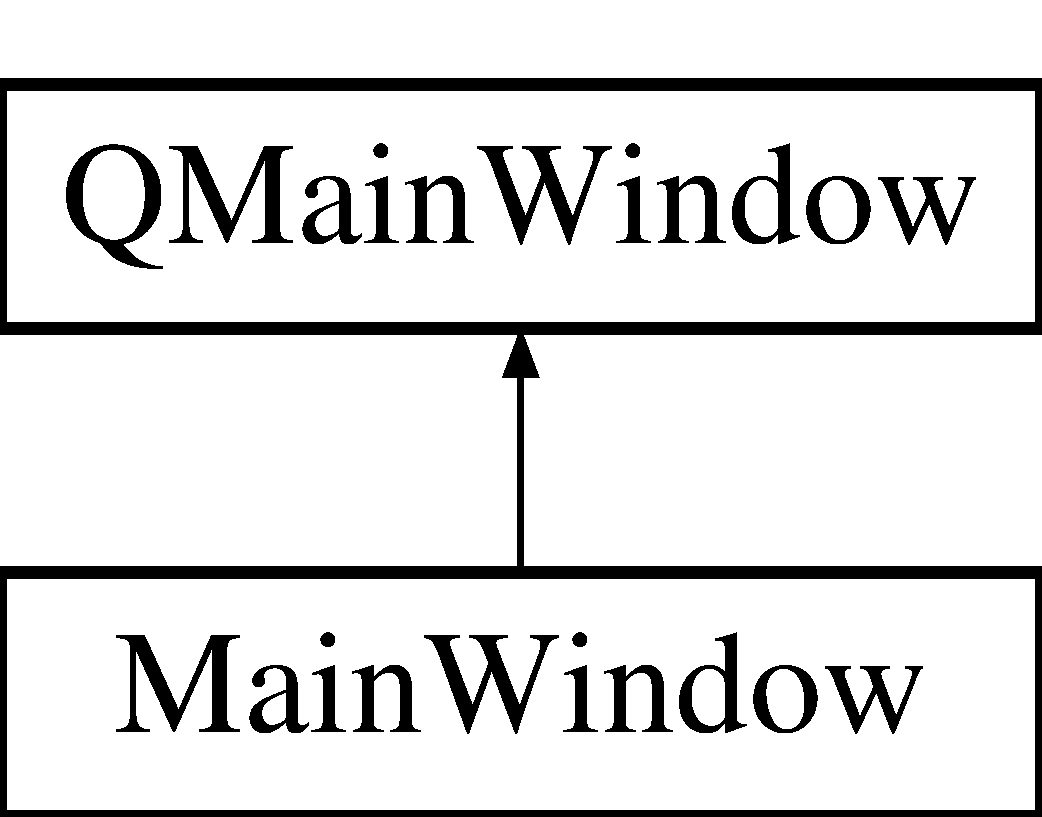
\includegraphics[height=2.000000cm]{classMainWindow}
\end{center}
\end{figure}
\subsection*{Public Slots}
\begin{DoxyCompactItemize}
\item 
\hypertarget{classMainWindow_ab2c0d4d0d84826cc032a45ea4783dde5}{}void {\bfseries Selected\+Item\+Change} ()\label{classMainWindow_ab2c0d4d0d84826cc032a45ea4783dde5}

\item 
\hypertarget{classMainWindow_a99f4fa67c708306ecac0eb351c6968d6}{}void {\bfseries manual\+Node\+Selection} (const Q\+String \&)\label{classMainWindow_a99f4fa67c708306ecac0eb351c6968d6}

\item 
\hypertarget{classMainWindow_af6253ec8c287b675a80e80bdd0ad31cc}{}void {\bfseries manual\+Element\+Selection} (const Q\+String \&)\label{classMainWindow_af6253ec8c287b675a80e80bdd0ad31cc}

\item 
\hypertarget{classMainWindow_ad613f2de4daee9c84828dc0490b00ffa}{}void {\bfseries Manual\+Element\+Selection\+Reset} ()\label{classMainWindow_ad613f2de4daee9c84828dc0490b00ffa}

\item 
\hypertarget{classMainWindow_a52630b918235794e8ff6cfd6abfc4b7f}{}void {\bfseries Manual\+Node\+Selection\+Reset} ()\label{classMainWindow_a52630b918235794e8ff6cfd6abfc4b7f}

\item 
\hypertarget{classMainWindow_a59dd1f2fe0d6900a98feff45c94e23e6}{}void {\bfseries timer\+Simulation\+Step} ()\label{classMainWindow_a59dd1f2fe0d6900a98feff45c94e23e6}

\item 
\hypertarget{classMainWindow_a0dce0c101c73abe3b5f347cd4dacfbd3}{}void {\bfseries update\+Strain} (int)\label{classMainWindow_a0dce0c101c73abe3b5f347cd4dacfbd3}

\item 
\hypertarget{classMainWindow_aae2aa15cd495069aebec712f4064c158}{}void {\bfseries update\+Myosin\+Combo\+Box} (int s)\label{classMainWindow_aae2aa15cd495069aebec712f4064c158}

\item 
\hypertarget{classMainWindow_a99a35d2b2c33a4cadab365403816c15c}{}void {\bfseries update\+Strain\+Check\+Box} (int)\label{classMainWindow_a99a35d2b2c33a4cadab365403816c15c}

\item 
\hypertarget{classMainWindow_a18d28bd55cc52f4b81d1c09e655d9711}{}void {\bfseries update\+Strain\+Spin\+Boxes} (double)\label{classMainWindow_a18d28bd55cc52f4b81d1c09e655d9711}

\item 
\hypertarget{classMainWindow_a524bf8d075a209be107c5ee9cd750bba}{}void {\bfseries update\+Pys\+Prop} (int s)\label{classMainWindow_a524bf8d075a209be107c5ee9cd750bba}

\item 
\hypertarget{classMainWindow_a933538d0ccf6de1298c6e4c7ed223f38}{}void {\bfseries update\+Pys\+Check\+Box} (int)\label{classMainWindow_a933538d0ccf6de1298c6e4c7ed223f38}

\item 
\hypertarget{classMainWindow_acd6a8996cd12c70a0e0572eebb9dc24d}{}void {\bfseries update\+Pys\+Prop\+Spin\+Boxes} (double d)\label{classMainWindow_acd6a8996cd12c70a0e0572eebb9dc24d}

\item 
\hypertarget{classMainWindow_ad30193e1dac5d64c7467e576e238ce03}{}void {\bfseries update\+Display\+Pipette} (int)\label{classMainWindow_ad30193e1dac5d64c7467e576e238ce03}

\item 
\hypertarget{classMainWindow_ac6e570780295db3ff54382cbda1ea4cf}{}void {\bfseries update\+Net\+Force\+Check\+Box} (int)\label{classMainWindow_ac6e570780295db3ff54382cbda1ea4cf}

\item 
\hypertarget{classMainWindow_a6d97f5be9f61304b31db8f83d11f6b8d}{}void {\bfseries update\+Myosin\+Check\+Box} (int)\label{classMainWindow_a6d97f5be9f61304b31db8f83d11f6b8d}

\item 
\hypertarget{classMainWindow_abf1716feb02925cadc40800ed5aa1af8}{}void {\bfseries update\+Packing\+Force\+Check\+Box} (int)\label{classMainWindow_abf1716feb02925cadc40800ed5aa1af8}

\item 
\hypertarget{classMainWindow_a0860bef7bbd9ae81c607142a8462e0a7}{}void {\bfseries update\+Velocity\+Check\+Box} (int)\label{classMainWindow_a0860bef7bbd9ae81c607142a8462e0a7}

\item 
\hypertarget{classMainWindow_af7f60ea4eea7ff11fd1f892455d86063}{}void {\bfseries update\+Scale\+Bar\+Check\+Box} (int)\label{classMainWindow_af7f60ea4eea7ff11fd1f892455d86063}

\item 
\hypertarget{classMainWindow_aee2509de2d13eedd782420cf86cd34d6}{}void {\bfseries update\+Peripodial\+Display\+Check\+Box} (int s)\label{classMainWindow_aee2509de2d13eedd782420cf86cd34d6}

\item 
\hypertarget{classMainWindow_a516111157b177a92fc5838a060f36908}{}void {\bfseries update\+Columnar\+Layer\+Display\+Check\+Box} (int s)\label{classMainWindow_a516111157b177a92fc5838a060f36908}

\item 
\hypertarget{classMainWindow_a52aa21a413bbc1f33a84f695b677f490}{}void {\bfseries update\+Bounding\+Box\+Check\+Box} (int s)\label{classMainWindow_a52aa21a413bbc1f33a84f695b677f490}

\item 
\hypertarget{classMainWindow_af2c325c24155eb2198ef705d78d452d8}{}void {\bfseries update\+Orthagonal\+Perspective\+View\+Toggle} ()\label{classMainWindow_af2c325c24155eb2198ef705d78d452d8}

\item 
\hypertarget{classMainWindow_a75a93ee195e391c9172bd77bb5eecd93}{}void {\bfseries update\+To\+Top\+View} ()\label{classMainWindow_a75a93ee195e391c9172bd77bb5eecd93}

\item 
\hypertarget{classMainWindow_a150680b802b4d7d5112209bd19cd3e5a}{}void {\bfseries update\+To\+Front\+View} ()\label{classMainWindow_a150680b802b4d7d5112209bd19cd3e5a}

\item 
\hypertarget{classMainWindow_a0a6e65fa32274c4a7fecb7ca04795388}{}void {\bfseries update\+To\+Side\+View} ()\label{classMainWindow_a0a6e65fa32274c4a7fecb7ca04795388}

\item 
\hypertarget{classMainWindow_a1607a9c35bde875a8218c763204e4fcf}{}void {\bfseries update\+To\+Perspective\+View} ()\label{classMainWindow_a1607a9c35bde875a8218c763204e4fcf}

\item 
\hypertarget{classMainWindow_a43031416fc2795d2b3cda8a158476549}{}void {\bfseries update\+Draw\+Symmetricity\+View\+Toggle} ()\label{classMainWindow_a43031416fc2795d2b3cda8a158476549}

\item 
\hypertarget{classMainWindow_ab677ef1bf70bc78faa5680576c14cd22}{}void {\bfseries x\+Clip\+Change} (int)\label{classMainWindow_ab677ef1bf70bc78faa5680576c14cd22}

\item 
\hypertarget{classMainWindow_a019023e11d09610ad8632baeb6854c61}{}void {\bfseries y\+Clip\+Change} (int)\label{classMainWindow_a019023e11d09610ad8632baeb6854c61}

\item 
\hypertarget{classMainWindow_af30a90f508a3d0b4434ddcaf848c69ac}{}void {\bfseries z\+Clip\+Change} (int)\label{classMainWindow_af30a90f508a3d0b4434ddcaf848c69ac}

\end{DoxyCompactItemize}
\subsection*{Public Member Functions}
\begin{DoxyCompactItemize}
\item 
\hypertarget{classMainWindow_aa1c3a3a33e1e67e055b8448ad9a9e208}{}{\bfseries Main\+Window} (\hyperlink{classSimulation}{Simulation} $\ast$S\+Im01)\label{classMainWindow_aa1c3a3a33e1e67e055b8448ad9a9e208}

\end{DoxyCompactItemize}
\subsection*{Public Attributes}
\begin{DoxyCompactItemize}
\item 
\hypertarget{classMainWindow_a9604326eab0369c7de6be01f992e0ba7}{}Q\+Graphics\+Scene $\ast$ {\bfseries Main\+Scene}\label{classMainWindow_a9604326eab0369c7de6be01f992e0ba7}

\item 
\hypertarget{classMainWindow_a80b2787fc058a3f5141b905d6c69c0ad}{}Q\+V\+Box\+Layout $\ast$ {\bfseries Control\+Panel\+Main\+H\+Box}\label{classMainWindow_a80b2787fc058a3f5141b905d6c69c0ad}

\item 
\hypertarget{classMainWindow_a028cf99e2842ca1250d4c103310c3430}{}Q\+Grid\+Layout $\ast$ {\bfseries Main\+Grid}\label{classMainWindow_a028cf99e2842ca1250d4c103310c3430}

\item 
\hypertarget{classMainWindow_aebd88a36f5ea16df9a037f7591090856}{}\hyperlink{classGLWidget}{G\+L\+Widget} $\ast$ {\bfseries Main\+G\+L\+Widget}\label{classMainWindow_aebd88a36f5ea16df9a037f7591090856}

\item 
\hypertarget{classMainWindow_aedd252a3fb1c0e6c7fe2d9edb5d19b83}{}\hyperlink{classSimulation}{Simulation} $\ast$ {\bfseries Sim01}\label{classMainWindow_aedd252a3fb1c0e6c7fe2d9edb5d19b83}

\end{DoxyCompactItemize}


The documentation for this class was generated from the following files\+:\begin{DoxyCompactItemize}
\item 
/home/melda/\+Documents/\+Tissue\+Folding/\+User\+Interface/\+Source\+Code/Main\+Window.\+h\item 
/home/melda/\+Documents/\+Tissue\+Folding/\+User\+Interface/\+Source\+Code/Main\+Window.\+cpp\end{DoxyCompactItemize}

\hypertarget{classModelInputObject}{}\section{Model\+Input\+Object Class Reference}
\label{classModelInputObject}\index{Model\+Input\+Object@{Model\+Input\+Object}}


{\ttfamily \#include $<$Model\+Input\+Object.\+h$>$}

\subsection*{Public Member Functions}
\begin{DoxyCompactItemize}
\item 
\hypertarget{classModelInputObject_a64b031469546b19177c0a13365058162}{}\hyperlink{classModelInputObject_a64b031469546b19177c0a13365058162}{Model\+Input\+Object} ()\label{classModelInputObject_a64b031469546b19177c0a13365058162}

\begin{DoxyCompactList}\small\item\em The constructor of the \hyperlink{classModelInputObject}{Model\+Input\+Object}. \end{DoxyCompactList}\item 
bool \hyperlink{classModelInputObject_a9741685527f446bd2bf66455c5b01d0c}{read\+Parameters} ()
\begin{DoxyCompactList}\small\item\em This is the main funciton reading the parameters from file. \end{DoxyCompactList}\end{DoxyCompactItemize}
\subsection*{Public Attributes}
\begin{DoxyCompactItemize}
\item 
\hypertarget{classModelInputObject_a0c5fb50d9d705bc9a9b4fafeebd1cadc}{}\hyperlink{classSimulation}{Simulation} $\ast$ \hyperlink{classModelInputObject_a0c5fb50d9d705bc9a9b4fafeebd1cadc}{Sim}\label{classModelInputObject_a0c5fb50d9d705bc9a9b4fafeebd1cadc}

\begin{DoxyCompactList}\small\item\em The pointer to the simulation object, for which the parameters are being read from the modelinput file. \end{DoxyCompactList}\item 
\hypertarget{classModelInputObject_a32fadb000159d03f6c5901ce3167ada8}{}const char $\ast$ \hyperlink{classModelInputObject_a32fadb000159d03f6c5901ce3167ada8}{parameter\+File\+Name}\label{classModelInputObject_a32fadb000159d03f6c5901ce3167ada8}

\begin{DoxyCompactList}\small\item\em The name (including path) of the file containing the model input parameters. \end{DoxyCompactList}\item 
\hypertarget{classModelInputObject_a2621e76abbd05573aea2d5471a589405}{}string \hyperlink{classModelInputObject_a2621e76abbd05573aea2d5471a589405}{mesh\+File\+Name}\label{classModelInputObject_a2621e76abbd05573aea2d5471a589405}

\begin{DoxyCompactList}\small\item\em The name (including path) of the file containing the input mesh file for tissue geometry. \end{DoxyCompactList}\end{DoxyCompactItemize}


\subsection{Detailed Description}
\hyperlink{classModelInputObject}{Model\+Input\+Object} class 

\subsection{Member Function Documentation}
\hypertarget{classModelInputObject_a9741685527f446bd2bf66455c5b01d0c}{}\index{Model\+Input\+Object@{Model\+Input\+Object}!read\+Parameters@{read\+Parameters}}
\index{read\+Parameters@{read\+Parameters}!Model\+Input\+Object@{Model\+Input\+Object}}
\subsubsection[{read\+Parameters}]{\setlength{\rightskip}{0pt plus 5cm}bool Model\+Input\+Object\+::read\+Parameters (
\begin{DoxyParamCaption}
{}
\end{DoxyParamCaption}
)}\label{classModelInputObject_a9741685527f446bd2bf66455c5b01d0c}


This is the main funciton reading the parameters from file. 

This function will read all available model inputs from the file \hyperlink{classModelInputObject_a32fadb000159d03f6c5901ce3167ada8}{Model\+Input\+Object\+::parameter\+File\+Name}. ~\newline
It will start by opening the model input file, after each attempt to open a file, there will be a health check to ensure the file could be opened. In case there are issues with the file (most common one being the file is not opened due to a path error), the function will throw an error with corresponding explanatory error message, and quit the simulation.

After successfully opening the input file, the function will read it until it reaches to the end of the file. This will involve a series of private functions, which are thoroughly documented in source code, while the processed documentation may or may not be available in this user interface documentation structure.

Depending on the header the function it encounters it will read\+:

Mesh geometry related parameters through the private function Model\+Input\+Object\+::read\+Mesh\+Parameters

Peripodial membrane structure related parameters through the private function Model\+Input\+Object\+::read\+Peripodial\+Membrane\+Parameters

Linker zone physical properties through the private function Model\+Input\+Object\+::read\+Linker\+Zone\+Parameters

Inputs relating to fixing the nodes of the tissue through the private function Model\+Input\+Object\+::read\+Node\+Fixing\+Parameters

Inputs relating to the external viscosity felt by the tissue through private function Model\+Input\+Object\+::read\+Eternal\+Viscosity\+Parameters

Inputs relating to manual manipulations to tissue after the mesh is read in

\hyperlink{classSimulation}{Simulation} time and time step related parameters through the private function Model\+Input\+Object\+::read\+Time\+Parameters

Physical parameters of the tissue through the private function Model\+Input\+Object\+::read\+Pysical\+Properties

Save options of the simulation through the private function Model\+Input\+Object\+::read\+Save\+Options

Growth functions and related parameters of the simulation through the private function Model\+Input\+Object\+::read\+Growth\+Options

Shape change functions and related parameters of the simulation through the private function Model\+Input\+Object\+::read\+Shape\+Change\+Options

Plastic deformation options through the private function Model\+Input\+Object\+::read\+Plastic\+Deformation\+Options

Myosin concentrations and related parameters of the simulation through the private function Model\+Input\+Object\+::read\+Myosin\+Options

Stretcher experimental setup parameters of the simulation through the private function Model\+Input\+Object\+::read\+Stretcher\+Setup

Pipette aspiration experimental setup parameters of the simulation through the private function Model\+Input\+Object\+::read\+Pipette\+Setup

In the case that the function, or any of the above listed parameter reading functions, encounters an unexpected line in the model input file, it will throw an error with a corresponding explanatory message, and quit the simulation.

The documentation for this class was generated from the following files\+:\begin{DoxyCompactItemize}
\item 
/home/melda/\+Documents/\+Tissue\+Folding/\+Tissue\+Folding/\+Source\+Code/Model\+Input\+Object.\+h\item 
/home/melda/\+Documents/\+Tissue\+Folding/\+Tissue\+Folding/\+Source\+Code/Model\+Input\+Object.\+cpp\end{DoxyCompactItemize}

\hypertarget{classMyosinFunction}{}\section{Myosin\+Function Class Reference}
\label{classMyosinFunction}\index{Myosin\+Function@{Myosin\+Function}}
\subsection*{Public Member Functions}
\begin{DoxyCompactItemize}
\item 
\hyperlink{classMyosinFunction_a25c83e1aaafc9d029e6c551008114ef7}{Myosin\+Function} (int id, bool \hyperlink{classMyosinFunction_a413c9a88624a97f6483efebdc5ab6fac}{is\+Apical}, bool \hyperlink{classMyosinFunction_a66bf31a5b46a19e67691d67b25c03852}{is\+Polarised}, int \hyperlink{classMyosinFunction_a5bf0e10f1e37ef01762fe72305d2e4d2}{init\+Time}, bool \hyperlink{classMyosinFunction_a6a978e5577af3f6b56edda5fd825d89c}{apply\+To\+Columnar\+Layer}, bool \hyperlink{classMyosinFunction_a76b32da8850a97ca48046d34542ee1c0}{apply\+To\+Peripodial\+Membrane}, int n\+X, int n\+Y, double $\ast$$\ast$Myo\+Mat, double $\ast$$\ast$angle\+Mat)
\begin{DoxyCompactList}\small\item\em The constructor of \hyperlink{classMyosinFunction}{Myosin\+Function}. Different growth functions will be derived from this class. \end{DoxyCompactList}\item 
\hyperlink{classMyosinFunction_a9a1d0f2da5bf8c9f3e9f48d88297c3fd}{Myosin\+Function} (int id, bool \hyperlink{classMyosinFunction_a413c9a88624a97f6483efebdc5ab6fac}{is\+Apical}, bool \hyperlink{classMyosinFunction_a66bf31a5b46a19e67691d67b25c03852}{is\+Polarised}, int \hyperlink{classMyosinFunction_a5bf0e10f1e37ef01762fe72305d2e4d2}{init\+Time}, bool \hyperlink{classMyosinFunction_a6a978e5577af3f6b56edda5fd825d89c}{apply\+To\+Columnar\+Layer}, bool \hyperlink{classMyosinFunction_a76b32da8850a97ca48046d34542ee1c0}{apply\+To\+Peripodial\+Membrane}, double stripe\+Size1, double stripe\+Size2, double initial\+Point, double end\+Point, double manualc\+Eq, double tetha)
\begin{DoxyCompactList}\small\item\em The constructor of \hyperlink{classMyosinFunction}{Myosin\+Function}. Different growth functions will be derived from this class. \end{DoxyCompactList}\item 
\hypertarget{classMyosinFunction_a81060aaa6923f43a5a9e2dcbb11a9ac6}{}int \hyperlink{classMyosinFunction_a81060aaa6923f43a5a9e2dcbb11a9ac6}{get\+Grid\+X} ()\label{classMyosinFunction_a81060aaa6923f43a5a9e2dcbb11a9ac6}

\begin{DoxyCompactList}\small\item\em This function returns \hyperlink{classMyosinFunction_a36ac0b5ce87011878a7f1954e270e5ae}{Myosin\+Function\+::n\+Grid\+X}. \end{DoxyCompactList}\item 
\hypertarget{classMyosinFunction_ab73e8b8b716defffabf6b3bf23d606d9}{}int \hyperlink{classMyosinFunction_ab73e8b8b716defffabf6b3bf23d606d9}{get\+Grid\+Y} ()\label{classMyosinFunction_ab73e8b8b716defffabf6b3bf23d606d9}

\begin{DoxyCompactList}\small\item\em This function returns \hyperlink{classMyosinFunction_a1652a8a0d154b136434bee037e0262a4}{Myosin\+Function\+::n\+Grid\+Y}. \end{DoxyCompactList}\item 
\hypertarget{classMyosinFunction_a59fb2bb53bf315ab2740ab27f7fa7536}{}double $\ast$$\ast$ \hyperlink{classMyosinFunction_a59fb2bb53bf315ab2740ab27f7fa7536}{get\+Equilibrium\+Myo\+Matrix} ()\label{classMyosinFunction_a59fb2bb53bf315ab2740ab27f7fa7536}

\begin{DoxyCompactList}\small\item\em This function returns Myosin\+Function\+::\+Growth\+Matrix. \end{DoxyCompactList}\item 
\hypertarget{classMyosinFunction_ac8b8b7bd3c067e83f36f42930c5fd45d}{}double \hyperlink{classMyosinFunction_ac8b8b7bd3c067e83f36f42930c5fd45d}{get\+Equilibrium\+Myo\+Matrix\+Element} (int i, int j)\label{classMyosinFunction_ac8b8b7bd3c067e83f36f42930c5fd45d}

\begin{DoxyCompactList}\small\item\em This function returns a the equilibrium myosin concentration at grid point \mbox{[}i\mbox{]}\mbox{[}j\mbox{]} (in dimensions \hyperlink{classMyosinFunction_a36ac0b5ce87011878a7f1954e270e5ae}{Myosin\+Function\+::n\+Grid\+X}, \hyperlink{classMyosinFunction_a1652a8a0d154b136434bee037e0262a4}{Myosin\+Function\+::n\+Grid\+Y}). \end{DoxyCompactList}\item 
\hypertarget{classMyosinFunction_a2249447e97be176009c74d34d5219498}{}double $\ast$$\ast$$\ast$ \hyperlink{classMyosinFunction_a2249447e97be176009c74d34d5219498}{get\+Orientation\+Matrix} ()\label{classMyosinFunction_a2249447e97be176009c74d34d5219498}

\begin{DoxyCompactList}\small\item\em This function returns \hyperlink{classMyosinFunction_a171909633b0117031045287fdbc401db}{Myosin\+Function\+::\+Myosin\+Orientation\+Matrix}. \end{DoxyCompactList}\item 
\hypertarget{classMyosinFunction_a5952daaeebe5fe284ecf096687d1c7c0}{}double \hyperlink{classMyosinFunction_a5952daaeebe5fe284ecf096687d1c7c0}{get\+Orientation\+Matrix\+Element} (int i, int j, int k)\label{classMyosinFunction_a5952daaeebe5fe284ecf096687d1c7c0}

\begin{DoxyCompactList}\small\item\em This function returns the myosin orientation at grid point \mbox{[}i\mbox{]}\mbox{[}j\mbox{]} (in dimensions \hyperlink{classMyosinFunction_a36ac0b5ce87011878a7f1954e270e5ae}{Myosin\+Function\+::n\+Grid\+X}, \hyperlink{classMyosinFunction_a1652a8a0d154b136434bee037e0262a4}{Myosin\+Function\+::n\+Grid\+Y} as in normalised vector \mbox{[} D\+V axis (x), A\+P axis (y)\mbox{]} ). \end{DoxyCompactList}\item 
\hypertarget{classMyosinFunction_a7f9b40f267049352619709243c929a25}{}void \hyperlink{classMyosinFunction_a7f9b40f267049352619709243c929a25}{set\+Orientation\+Matrix\+Element} (double ex, double ey, int i, int j)\label{classMyosinFunction_a7f9b40f267049352619709243c929a25}

\begin{DoxyCompactList}\small\item\em This function sets the myosin orientation at grid point \mbox{[}i\mbox{]}\mbox{[}j\mbox{]} (in dimensions \hyperlink{classMyosinFunction_a36ac0b5ce87011878a7f1954e270e5ae}{Myosin\+Function\+::n\+Grid\+X}, \hyperlink{classMyosinFunction_a1652a8a0d154b136434bee037e0262a4}{Myosin\+Function\+::n\+Grid\+Y}), to the growth rate \mbox{[}ex, ez\mbox{]} in the format \mbox{[} D\+V axis (x), A\+P axis (y)\mbox{]} The vector M\+U\+S\+T be normalised. \end{DoxyCompactList}\item 
void \hyperlink{classMyosinFunction_ad0bfc8aafe7e54a46f04e8eeb84ce457}{write\+Summary} (ofstream \&save\+File\+Simulation\+Summary)
\begin{DoxyCompactList}\small\item\em The. \end{DoxyCompactList}\end{DoxyCompactItemize}
\subsection*{Public Attributes}
\begin{DoxyCompactItemize}
\item 
\hypertarget{classMyosinFunction_a718e298e9ed8eee2b037fd08d7bd4373}{}int \hyperlink{classMyosinFunction_a718e298e9ed8eee2b037fd08d7bd4373}{Id}\label{classMyosinFunction_a718e298e9ed8eee2b037fd08d7bd4373}

\begin{DoxyCompactList}\small\item\em The unique identification number of the myosin function. \end{DoxyCompactList}\item 
\hypertarget{classMyosinFunction_a5bf0e10f1e37ef01762fe72305d2e4d2}{}int \hyperlink{classMyosinFunction_a5bf0e10f1e37ef01762fe72305d2e4d2}{init\+Time}\label{classMyosinFunction_a5bf0e10f1e37ef01762fe72305d2e4d2}

\begin{DoxyCompactList}\small\item\em The application time of the myosin response, in time steps. If the input value(sec) does not fit with the time steps, it will be rounded down. \end{DoxyCompactList}\item 
\hypertarget{classMyosinFunction_a413c9a88624a97f6483efebdc5ab6fac}{}bool \hyperlink{classMyosinFunction_a413c9a88624a97f6483efebdc5ab6fac}{is\+Apical}\label{classMyosinFunction_a413c9a88624a97f6483efebdc5ab6fac}

\begin{DoxyCompactList}\small\item\em The boolean stating if the myosin function is for the apical surface of selected tissue layer. \end{DoxyCompactList}\item 
\hypertarget{classMyosinFunction_a66bf31a5b46a19e67691d67b25c03852}{}bool \hyperlink{classMyosinFunction_a66bf31a5b46a19e67691d67b25c03852}{is\+Polarised}\label{classMyosinFunction_a66bf31a5b46a19e67691d67b25c03852}

\begin{DoxyCompactList}\small\item\em The boolean stating if the myosin function is is polarised, defaul value is false, and applies a uniform contraction of the surface. \end{DoxyCompactList}\item 
\hypertarget{classMyosinFunction_a6a978e5577af3f6b56edda5fd825d89c}{}bool \hyperlink{classMyosinFunction_a6a978e5577af3f6b56edda5fd825d89c}{apply\+To\+Columnar\+Layer}\label{classMyosinFunction_a6a978e5577af3f6b56edda5fd825d89c}

\begin{DoxyCompactList}\small\item\em Boolean stating if the myosin levels should be applied to columnar layer. \end{DoxyCompactList}\item 
\hypertarget{classMyosinFunction_a76b32da8850a97ca48046d34542ee1c0}{}bool \hyperlink{classMyosinFunction_a76b32da8850a97ca48046d34542ee1c0}{apply\+To\+Peripodial\+Membrane}\label{classMyosinFunction_a76b32da8850a97ca48046d34542ee1c0}

\begin{DoxyCompactList}\small\item\em Boolean stating if the myosin levels should be applied to peripodial membrane. \end{DoxyCompactList}\item 
\hypertarget{classMyosinFunction_af9847dcd6e9db66662d90e3e4ba4cc0b}{}bool {\bfseries manual\+Stripes}\label{classMyosinFunction_af9847dcd6e9db66662d90e3e4ba4cc0b}

\item 
\hypertarget{classMyosinFunction_aae36807a55b8886c6ebfe24598a160ea}{}double {\bfseries stripe\+Size1}\label{classMyosinFunction_aae36807a55b8886c6ebfe24598a160ea}

\item 
\hypertarget{classMyosinFunction_a540d49e3dbb0b6b119eebfa3d3dcb4bb}{}double {\bfseries stripe\+Size2}\label{classMyosinFunction_a540d49e3dbb0b6b119eebfa3d3dcb4bb}

\item 
\hypertarget{classMyosinFunction_a71b4c116055c970cd05c4ecd9fbeca6a}{}double {\bfseries initial\+Point}\label{classMyosinFunction_a71b4c116055c970cd05c4ecd9fbeca6a}

\item 
\hypertarget{classMyosinFunction_a21f2a844af80cb09c37fbc9b20909c7f}{}double {\bfseries end\+Point}\label{classMyosinFunction_a21f2a844af80cb09c37fbc9b20909c7f}

\item 
\hypertarget{classMyosinFunction_acfa8ebd891b11162a806a8ebf9b6f39a}{}double {\bfseries manual\+C\+Myo\+Eq}\label{classMyosinFunction_acfa8ebd891b11162a806a8ebf9b6f39a}

\item 
\hypertarget{classMyosinFunction_a8e71a34d5be53e6eb7c1d3621fe72455}{}double {\bfseries manual\+Orientation} \mbox{[}2\mbox{]}\label{classMyosinFunction_a8e71a34d5be53e6eb7c1d3621fe72455}

\item 
\hypertarget{classMyosinFunction_a36ac0b5ce87011878a7f1954e270e5ae}{}int \hyperlink{classMyosinFunction_a36ac0b5ce87011878a7f1954e270e5ae}{n\+Grid\+X}\label{classMyosinFunction_a36ac0b5ce87011878a7f1954e270e5ae}

\begin{DoxyCompactList}\small\item\em The number of grid points that discretise the tissue in x. \end{DoxyCompactList}\item 
\hypertarget{classMyosinFunction_a1652a8a0d154b136434bee037e0262a4}{}int \hyperlink{classMyosinFunction_a1652a8a0d154b136434bee037e0262a4}{n\+Grid\+Y}\label{classMyosinFunction_a1652a8a0d154b136434bee037e0262a4}

\begin{DoxyCompactList}\small\item\em The number of grid points that discretise the tissue in y. \end{DoxyCompactList}\item 
\hypertarget{classMyosinFunction_a7332175e6d9369c02a8c569f000211e1}{}double $\ast$$\ast$ \hyperlink{classMyosinFunction_a7332175e6d9369c02a8c569f000211e1}{Equilibrium\+Myosin\+Matrix}\label{classMyosinFunction_a7332175e6d9369c02a8c569f000211e1}

\begin{DoxyCompactList}\small\item\em The matrix of equilibrium myosin levels. It is a matrix of doubles for equilibrium concentration at each grid point. The dimensions of the matrix are equal to (\hyperlink{classMyosinFunction_a36ac0b5ce87011878a7f1954e270e5ae}{Myosin\+Function\+::n\+Grid\+X}, \hyperlink{classMyosinFunction_a1652a8a0d154b136434bee037e0262a4}{Myosin\+Function\+::n\+Grid\+Y}), and set in constructor of the \hyperlink{classMyosinFunction}{Myosin\+Function}. \end{DoxyCompactList}\item 
\hypertarget{classMyosinFunction_a171909633b0117031045287fdbc401db}{}double $\ast$$\ast$$\ast$ \hyperlink{classMyosinFunction_a171909633b0117031045287fdbc401db}{Myosin\+Orientation\+Matrix}\label{classMyosinFunction_a171909633b0117031045287fdbc401db}

\begin{DoxyCompactList}\small\item\em The matrix of equilibrium myosin orientations. It is a matrix of double triplets for equilibrium orientation at each grid point. The dimensions of the matrix are equal to (\hyperlink{classMyosinFunction_a36ac0b5ce87011878a7f1954e270e5ae}{Myosin\+Function\+::n\+Grid\+X} \mbox{[}3\mbox{]}, \hyperlink{classMyosinFunction_a1652a8a0d154b136434bee037e0262a4}{Myosin\+Function\+::n\+Grid\+Y} \mbox{[}3\mbox{]}), and set in constructor of the \hyperlink{classMyosinFunction}{Myosin\+Function}. \end{DoxyCompactList}\end{DoxyCompactItemize}


\subsection{Constructor \& Destructor Documentation}
\hypertarget{classMyosinFunction_a25c83e1aaafc9d029e6c551008114ef7}{}\index{Myosin\+Function@{Myosin\+Function}!Myosin\+Function@{Myosin\+Function}}
\index{Myosin\+Function@{Myosin\+Function}!Myosin\+Function@{Myosin\+Function}}
\subsubsection[{Myosin\+Function}]{\setlength{\rightskip}{0pt plus 5cm}Myosin\+Function\+::\+Myosin\+Function (
\begin{DoxyParamCaption}
\item[{int}]{id, }
\item[{bool}]{is\+Apical, }
\item[{bool}]{is\+Polarised, }
\item[{int}]{init\+Time, }
\item[{bool}]{apply\+To\+Columnar\+Layer, }
\item[{bool}]{apply\+To\+Peripodial\+Membrane, }
\item[{int}]{n\+X, }
\item[{int}]{n\+Y, }
\item[{double $\ast$$\ast$}]{Myo\+Mat, }
\item[{double $\ast$$\ast$}]{angle\+Mat}
\end{DoxyParamCaption}
)\hspace{0.3cm}{\ttfamily [inline]}}\label{classMyosinFunction_a25c83e1aaafc9d029e6c551008114ef7}


The constructor of \hyperlink{classMyosinFunction}{Myosin\+Function}. Different growth functions will be derived from this class. 

The first six parameters will be directed to the parent constructor, \hyperlink{classGrowthFunctionBase_a061b31ad8a0cb228628c7104029a94bf}{Growth\+Function\+Base\+::\+Growth\+Function\+Base}. ~\newline
integers n\+X and n\+Y will set \hyperlink{classGridBasedGrowthFunction_af872b9963f3a579dcd615c23bcb58a86}{Grid\+Based\+Growth\+Function\+::n\+Grid\+X} and \hyperlink{classGridBasedGrowthFunction_a625bc963a1f1e7d1f1a35dbd0ef51728}{Grid\+Based\+Growth\+Function\+::n\+Grid\+Y}, respectively. \hyperlink{classGridBasedGrowthFunction_a5522d9b84fa95ebd65cdf290a4f0a65c}{Grid\+Based\+Growth\+Function\+::\+Growth\+Matrix} will be initiated to point at a 2 dimensional matrix of double triplets the size(n\+X, n\+Y). ~\newline
double$\ast$$\ast$$\ast$ Growth\+Mat is the pointer to the 2-\/dimensional matrix of double triplets, holding the 3\+D growth rates at each grid point. Values stored in Growth\+Mat will set the values in \hyperlink{classGridBasedGrowthFunction_a5522d9b84fa95ebd65cdf290a4f0a65c}{Grid\+Based\+Growth\+Function\+::\+Growth\+Matrix}. The matrix storing the growth rates have been read from an input file through Model\+Input\+Object\+::read\+Growth\+Options and related functions therein ~\newline
 \hypertarget{classMyosinFunction_a9a1d0f2da5bf8c9f3e9f48d88297c3fd}{}\index{Myosin\+Function@{Myosin\+Function}!Myosin\+Function@{Myosin\+Function}}
\index{Myosin\+Function@{Myosin\+Function}!Myosin\+Function@{Myosin\+Function}}
\subsubsection[{Myosin\+Function}]{\setlength{\rightskip}{0pt plus 5cm}Myosin\+Function\+::\+Myosin\+Function (
\begin{DoxyParamCaption}
\item[{int}]{id, }
\item[{bool}]{is\+Apical, }
\item[{bool}]{is\+Polarised, }
\item[{int}]{init\+Time, }
\item[{bool}]{apply\+To\+Columnar\+Layer, }
\item[{bool}]{apply\+To\+Peripodial\+Membrane, }
\item[{double}]{stripe\+Size1, }
\item[{double}]{stripe\+Size2, }
\item[{double}]{initial\+Point, }
\item[{double}]{end\+Point, }
\item[{double}]{manualc\+Eq, }
\item[{double}]{tetha}
\end{DoxyParamCaption}
)\hspace{0.3cm}{\ttfamily [inline]}}\label{classMyosinFunction_a9a1d0f2da5bf8c9f3e9f48d88297c3fd}


The constructor of \hyperlink{classMyosinFunction}{Myosin\+Function}. Different growth functions will be derived from this class. 

The first six parameters will be directed to the parent constructor, \hyperlink{classGrowthFunctionBase_a061b31ad8a0cb228628c7104029a94bf}{Growth\+Function\+Base\+::\+Growth\+Function\+Base}. ~\newline
integers n\+X and n\+Y will set \hyperlink{classGridBasedGrowthFunction_af872b9963f3a579dcd615c23bcb58a86}{Grid\+Based\+Growth\+Function\+::n\+Grid\+X} and \hyperlink{classGridBasedGrowthFunction_a625bc963a1f1e7d1f1a35dbd0ef51728}{Grid\+Based\+Growth\+Function\+::n\+Grid\+Y}, respectively. \hyperlink{classGridBasedGrowthFunction_a5522d9b84fa95ebd65cdf290a4f0a65c}{Grid\+Based\+Growth\+Function\+::\+Growth\+Matrix} will be initiated to point at a 2 dimensional matrix of double triplets the size(n\+X, n\+Y). ~\newline
double$\ast$$\ast$$\ast$ Growth\+Mat is the pointer to the 2-\/dimensional matrix of double triplets, holding the 3\+D growth rates at each grid point. Values stored in Growth\+Mat will set the values in \hyperlink{classGridBasedGrowthFunction_a5522d9b84fa95ebd65cdf290a4f0a65c}{Grid\+Based\+Growth\+Function\+::\+Growth\+Matrix}. The matrix storing the growth rates have been read from an input file through Model\+Input\+Object\+::read\+Growth\+Options and related functions therein ~\newline
 

\subsection{Member Function Documentation}
\hypertarget{classMyosinFunction_ad0bfc8aafe7e54a46f04e8eeb84ce457}{}\index{Myosin\+Function@{Myosin\+Function}!write\+Summary@{write\+Summary}}
\index{write\+Summary@{write\+Summary}!Myosin\+Function@{Myosin\+Function}}
\subsubsection[{write\+Summary}]{\setlength{\rightskip}{0pt plus 5cm}void Myosin\+Function\+::write\+Summary (
\begin{DoxyParamCaption}
\item[{ofstream \&}]{save\+File\+Simulation\+Summary}
\end{DoxyParamCaption}
)\hspace{0.3cm}{\ttfamily [inline]}}\label{classMyosinFunction_ad0bfc8aafe7e54a46f04e8eeb84ce457}


The. 

This function will write the \hyperlink{classMyosinFunction}{Myosin\+Function} details into the simulation summary file, provided as the first input. The output should look like\+: ~\newline
 Growth Type\+: growth From File (3) Initial time(sec)\+: \hyperlink{classGrowthFunctionBase_ae92513a7b41637df8e26e7db35ddf97c}{Grid\+Based\+Growth\+Function\+::init\+Time} Final\+Time time(sec)\+: \hyperlink{classGrowthFunctionBase_a3ff4db0573d354a75666a5f3ca446941}{Grid\+Based\+Growth\+Function\+::end\+Time} Growth matrix mesh size\+: \hyperlink{classGridBasedGrowthFunction_af872b9963f3a579dcd615c23bcb58a86}{Grid\+Based\+Growth\+Function\+::n\+Grid\+X} \hyperlink{classGridBasedGrowthFunction_a625bc963a1f1e7d1f1a35dbd0ef51728}{Grid\+Based\+Growth\+Function\+::n\+Grid\+Y}

The documentation for this class was generated from the following file\+:\begin{DoxyCompactItemize}
\item 
/home/melda/\+Documents/\+Tissue\+Folding/\+Tissue\+Folding/\+Source\+Code/Myosin\+Function.\+h\end{DoxyCompactItemize}

\hypertarget{classNode}{}\section{Node Class Reference}
\label{classNode}\index{Node@{Node}}


{\ttfamily \#include $<$Node.\+h$>$}

\subsection*{Public Member Functions}
\begin{DoxyCompactItemize}
\item 
\hypertarget{classNode_ac84926c5a9cf2883665f00382781b932}{}{\bfseries Node} (int id, int dim, double $\ast$pos, int tissue\+Pos, int \hyperlink{classNode_ae621097f98f1d33d283cf65a0a02d29a}{tissue\+Type})\label{classNode_ac84926c5a9cf2883665f00382781b932}

\item 
void \hyperlink{classNode_a9a3b878b16fe5be6ee707a49f3fd7d5a}{set\+External\+Viscosity} (double Apical\+Visc, double Basal\+Visc)
\begin{DoxyCompactList}\small\item\em The function to set the viscosity of the node. \end{DoxyCompactList}\item 
bool \hyperlink{classNode_a7dc5a9838a0a1963e58f648c5f7cb635}{check\+If\+Neighbour} (int Id\+To\+Check)
\begin{DoxyCompactList}\small\item\em The function to check if the node with input Id (Id\+To\+Check) is an immediate neighbour of the owner node. \end{DoxyCompactList}\item 
bool \hyperlink{classNode_a1d80e6f467d8ca919872b6e47a882dd5}{check\+If\+Node\+Has\+Packing} ()
\begin{DoxyCompactList}\small\item\em The function to check if the node is eligible for packing. \end{DoxyCompactList}\item 
void \hyperlink{classNode_ae4a2d9e601432a998efe24e1ac4a86cd}{get\+Current\+Position} (double $\ast$pos)
\begin{DoxyCompactList}\small\item\em return the current position of the node \end{DoxyCompactList}\item 
void \hyperlink{classNode_a3030a518aa97bd50060b8733e87540f7}{display\+Connected\+Element\+Ids} ()
\begin{DoxyCompactList}\small\item\em This function will print out a list of connected element Id\textquotesingle{}s. \end{DoxyCompactList}\item 
void \hyperlink{classNode_a755e8c3d76e7f1f0ab364fc3d4da3a9a}{display\+Connected\+Element\+Weights} ()
\begin{DoxyCompactList}\small\item\em This function will print out the weights of the connected elements, in the order of Id s given in connected\+Element\+Ids. \end{DoxyCompactList}\end{DoxyCompactItemize}
\subsection*{Public Attributes}
\begin{DoxyCompactItemize}
\item 
\hypertarget{classNode_a80edc54e934bdfc08b66933d4c7fd6f4}{}bool $\ast$ \hyperlink{classNode_a80edc54e934bdfc08b66933d4c7fd6f4}{Fixed\+Pos}\label{classNode_a80edc54e934bdfc08b66933d4c7fd6f4}

\begin{DoxyCompactList}\small\item\em The boolean array stating if the node\textquotesingle{}s position is fixed in any direction, format\+: \mbox{[}x y z\mbox{]}, true = fixed. \end{DoxyCompactList}\item 
\hypertarget{classNode_a1bd379569cc1a8b96432e61971aed4d9}{}int \hyperlink{classNode_a1bd379569cc1a8b96432e61971aed4d9}{Id}\label{classNode_a1bd379569cc1a8b96432e61971aed4d9}

\begin{DoxyCompactList}\small\item\em The unique identification number of the node. \end{DoxyCompactList}\item 
\hypertarget{classNode_ae23958d63ecbf80559c307c955be8227}{}int \hyperlink{classNode_ae23958d63ecbf80559c307c955be8227}{n\+Dim}\label{classNode_ae23958d63ecbf80559c307c955be8227}

\begin{DoxyCompactList}\small\item\em The number of dimensions of the node, (2 or 3) \end{DoxyCompactList}\item 
\hypertarget{classNode_a8fdca7042dc0cc7e342eb3c87cbbfb56}{}double $\ast$ \hyperlink{classNode_a8fdca7042dc0cc7e342eb3c87cbbfb56}{Position}\label{classNode_a8fdca7042dc0cc7e342eb3c87cbbfb56}

\begin{DoxyCompactList}\small\item\em The pointer to the position array of the node. The array itself is declared within the constructor, depending on n\+Dim. \end{DoxyCompactList}\item 
\hypertarget{classNode_abfa97f5fa4e95c932b4e3e0daabb062a}{}double $\ast$ \hyperlink{classNode_abfa97f5fa4e95c932b4e3e0daabb062a}{R\+K\+Position}\label{classNode_abfa97f5fa4e95c932b4e3e0daabb062a}

\begin{DoxyCompactList}\small\item\em The pointer to the position array for position during a Runge-\/\+Kutta step array of the node. The array itself is declared within the constructor, depending on n\+Dim. \end{DoxyCompactList}\item 
\hypertarget{classNode_ac27dee69b570030aacf8865190879845}{}double $\ast$$\ast$ \hyperlink{classNode_ac27dee69b570030aacf8865190879845}{Velocity}\label{classNode_ac27dee69b570030aacf8865190879845}

\begin{DoxyCompactList}\small\item\em The pointer($\ast$$\ast$) to the velocities of the node for each Runge-\/\+Kutta step. The final calculated velocity is stored in Velocity\mbox{[}0\mbox{]}. \end{DoxyCompactList}\item 
\hypertarget{classNode_a03f2f0310bec3504b082d0f707fa3db2}{}bool \hyperlink{classNode_a03f2f0310bec3504b082d0f707fa3db2}{external\+Viscosity\+Set\+In\+Fixing} \mbox{[}3\mbox{]}\label{classNode_a03f2f0310bec3504b082d0f707fa3db2}

\begin{DoxyCompactList}\small\item\em The boolean array stating if the external viscosity of any axis has been set in node fixing options. The node fixing is carried out before the physical parameter settings in most cases. The boolean check is carried out not to overwrite the existing set viscosity in normal viscosity assignment. \end{DoxyCompactList}\item 
\hypertarget{classNode_a9bb34133d43eb0f29bfd0d0b65df395d}{}double \hyperlink{classNode_a9bb34133d43eb0f29bfd0d0b65df395d}{external\+Viscosity} \mbox{[}3\mbox{]}\label{classNode_a9bb34133d43eb0f29bfd0d0b65df395d}

\begin{DoxyCompactList}\small\item\em External viscosity of the node, defined by its placement within the tissue. This can be defined as an external adhesion, E\+C\+M remodelling, or any other form of viscosity. \end{DoxyCompactList}\item 
\hypertarget{classNode_af754322e3928dc45f70b19762551890a}{}int \hyperlink{classNode_af754322e3928dc45f70b19762551890a}{tissue\+Placement}\label{classNode_af754322e3928dc45f70b19762551890a}

\begin{DoxyCompactList}\small\item\em The tissue placement is 0 for basal nodes, 1 for apical nodes, and 2 for middle range. \end{DoxyCompactList}\item 
\hypertarget{classNode_ae621097f98f1d33d283cf65a0a02d29a}{}int \hyperlink{classNode_ae621097f98f1d33d283cf65a0a02d29a}{tissue\+Type}\label{classNode_ae621097f98f1d33d283cf65a0a02d29a}

\begin{DoxyCompactList}\small\item\em The tissue type is 0 for columnar layer, 1 for peripodial membrane, and 2 for linker zone. \end{DoxyCompactList}\item 
\hypertarget{classNode_ab6b225354ad961f2e9bd5d7fe9b67b3a}{}bool \hyperlink{classNode_ab6b225354ad961f2e9bd5d7fe9b67b3a}{at\+Circumference}\label{classNode_ab6b225354ad961f2e9bd5d7fe9b67b3a}

\begin{DoxyCompactList}\small\item\em Boolean defining if the node is at the circumference of the columnar layer of the tissue. \end{DoxyCompactList}\item 
\hypertarget{classNode_a63e510fc9158eb15e751861bc14eae38}{}double \hyperlink{classNode_a63e510fc9158eb15e751861bc14eae38}{mass}\label{classNode_a63e510fc9158eb15e751861bc14eae38}

\begin{DoxyCompactList}\small\item\em The mass of the node, calculated via the elements that use the node as a vertex. \end{DoxyCompactList}\item 
\hypertarget{classNode_aab30ea418838635c21593c47f39f2699}{}double \hyperlink{classNode_aab30ea418838635c21593c47f39f2699}{surface}\label{classNode_aab30ea418838635c21593c47f39f2699}

\begin{DoxyCompactList}\small\item\em The surface of the node, calculated via apical or basal elements. Lateral surfaces are not included. \end{DoxyCompactList}\item 
\hypertarget{classNode_af8e9678dfeffc9e99d925a83b58fde3d}{}double \hyperlink{classNode_af8e9678dfeffc9e99d925a83b58fde3d}{z\+Projected\+Area}\label{classNode_af8e9678dfeffc9e99d925a83b58fde3d}

\begin{DoxyCompactList}\small\item\em The surface of the node, as projected in Z, calculated from apical or pasal surfces of elements, lateral surfaces are not included. \end{DoxyCompactList}\item 
\hypertarget{classNode_ab22060fb9f61a0d93ec52e6045828782}{}vector$<$ int $>$ \hyperlink{classNode_ab22060fb9f61a0d93ec52e6045828782}{immediate\+Neigs}\label{classNode_ab22060fb9f61a0d93ec52e6045828782}

\begin{DoxyCompactList}\small\item\em The list of Id\textquotesingle{}s for immediate neighbours of the node, i.\+e. the nodes that are shared by the elements that utilise the owner of this node. \end{DoxyCompactList}\item 
\hypertarget{classNode_a18bae606efb025cc90b4c117776e0bf9}{}vector$<$ int $>$ \hyperlink{classNode_a18bae606efb025cc90b4c117776e0bf9}{connected\+Element\+Ids}\label{classNode_a18bae606efb025cc90b4c117776e0bf9}

\begin{DoxyCompactList}\small\item\em The list of Id\textquotesingle{}s for elements that are utilising this node. \end{DoxyCompactList}\item 
\hypertarget{classNode_a7ffccd2a70d08c1a42d4701f32a266c5}{}vector$<$ double $>$ \hyperlink{classNode_a7ffccd2a70d08c1a42d4701f32a266c5}{connected\+Element\+Weights}\label{classNode_a7ffccd2a70d08c1a42d4701f32a266c5}

\begin{DoxyCompactList}\small\item\em The list of weights (normalised mass) for elements that are utilising this node, order is linked to \hyperlink{classNode_a18bae606efb025cc90b4c117776e0bf9}{Node\+::connected\+Element\+Ids}. \end{DoxyCompactList}\item 
\hypertarget{classNode_ad29e0f81f8c0a5d4a3e891d3b239af7e}{}int \hyperlink{classNode_ad29e0f81f8c0a5d4a3e891d3b239af7e}{symmetric\+Equivalent\+Id}\label{classNode_ad29e0f81f8c0a5d4a3e891d3b239af7e}

\begin{DoxyCompactList}\small\item\em The id of the node that this node will move symmetrically in y, if the tissue is symmetric and only half is simulated. \end{DoxyCompactList}\item 
\hypertarget{classNode_a71d38b47678cff15e338f9c917d32696}{}bool \hyperlink{classNode_a71d38b47678cff15e338f9c917d32696}{has\+Lateral\+Element\+Owner}\label{classNode_a71d38b47678cff15e338f9c917d32696}

\begin{DoxyCompactList}\small\item\em The boolean stating if any lateral element uses this node. \end{DoxyCompactList}\item 
\hypertarget{classNode_ae14618d71e657039ed84316154be7330}{}bool \hyperlink{classNode_ae14618d71e657039ed84316154be7330}{at\+Symmetricity\+Border}\label{classNode_ae14618d71e657039ed84316154be7330}

\begin{DoxyCompactList}\small\item\em The boolean stating if the node is at the border of symmetricity. \end{DoxyCompactList}\end{DoxyCompactItemize}


\subsection{Detailed Description}
The node class 

\subsection{Member Function Documentation}
\hypertarget{classNode_a7dc5a9838a0a1963e58f648c5f7cb635}{}\index{Node@{Node}!check\+If\+Neighbour@{check\+If\+Neighbour}}
\index{check\+If\+Neighbour@{check\+If\+Neighbour}!Node@{Node}}
\subsubsection[{check\+If\+Neighbour}]{\setlength{\rightskip}{0pt plus 5cm}bool Node\+::check\+If\+Neighbour (
\begin{DoxyParamCaption}
\item[{int}]{Id\+To\+Check}
\end{DoxyParamCaption}
)}\label{classNode_a7dc5a9838a0a1963e58f648c5f7cb635}


The function to check if the node with input Id (Id\+To\+Check) is an immediate neighbour of the owner node. 

This node will take in the apical columnar layer, basal columnar layer, and peripodial membrane viscosities of the tissue as inputs, respectively. The external viscosity of the node will be assigned via its \hyperlink{classNode_af754322e3928dc45f70b19762551890a}{Node\+::tissue\+Placement} and \hyperlink{classNode_ae621097f98f1d33d283cf65a0a02d29a}{Node\+::tissue\+Type}. On the columnar layer, nodes that are in the mid-\/zone of the tissue (neither on the apical nor on the basal surface, will take the average of the two values. The function will return true if the node with the unique \hyperlink{classNode_a1bd379569cc1a8b96432e61971aed4d9}{Node\+::\+Id} equal to \char`\"{}\+Id\+To\+Check\char`\"{} is an immediate neighbour of the current node. The search will be done through the list \hyperlink{classNode_ab22060fb9f61a0d93ec52e6045828782}{Node\+::immediate\+Neigs}\hypertarget{classNode_a1d80e6f467d8ca919872b6e47a882dd5}{}\index{Node@{Node}!check\+If\+Node\+Has\+Packing@{check\+If\+Node\+Has\+Packing}}
\index{check\+If\+Node\+Has\+Packing@{check\+If\+Node\+Has\+Packing}!Node@{Node}}
\subsubsection[{check\+If\+Node\+Has\+Packing}]{\setlength{\rightskip}{0pt plus 5cm}bool Node\+::check\+If\+Node\+Has\+Packing (
\begin{DoxyParamCaption}
{}
\end{DoxyParamCaption}
)}\label{classNode_a1d80e6f467d8ca919872b6e47a882dd5}


The function to check if the node is eligible for packing. 

The function will return true if the node is eligible for packing calculation. This packing will ensure volume exclusion, and is calculated via function \hyperlink{classSimulation_a51cb5448f660eeefc54a5d2a33ab561e}{Simulation\+::calculate\+Packing}. It is not necessary to calculate packing under the following conditions\+: 1) The node is at the middle of the columnar layer, the packing should have stopped any other node/element coming close enough to this node, as they would need to penetrate through the apical or basal surface of the tissue to reach this node.\hypertarget{classNode_a3030a518aa97bd50060b8733e87540f7}{}\index{Node@{Node}!display\+Connected\+Element\+Ids@{display\+Connected\+Element\+Ids}}
\index{display\+Connected\+Element\+Ids@{display\+Connected\+Element\+Ids}!Node@{Node}}
\subsubsection[{display\+Connected\+Element\+Ids}]{\setlength{\rightskip}{0pt plus 5cm}void Node\+::display\+Connected\+Element\+Ids (
\begin{DoxyParamCaption}
{}
\end{DoxyParamCaption}
)}\label{classNode_a3030a518aa97bd50060b8733e87540f7}


This function will print out a list of connected element Id\textquotesingle{}s. 

The function will display on screen the list of unique \hyperlink{classNode_a1bd379569cc1a8b96432e61971aed4d9}{Node\+::\+Id} s for the elements utilising this node. These elements are listed in \hyperlink{classNode_a18bae606efb025cc90b4c117776e0bf9}{Node\+::connected\+Element\+Ids}.\hypertarget{classNode_a755e8c3d76e7f1f0ab364fc3d4da3a9a}{}\index{Node@{Node}!display\+Connected\+Element\+Weights@{display\+Connected\+Element\+Weights}}
\index{display\+Connected\+Element\+Weights@{display\+Connected\+Element\+Weights}!Node@{Node}}
\subsubsection[{display\+Connected\+Element\+Weights}]{\setlength{\rightskip}{0pt plus 5cm}void Node\+::display\+Connected\+Element\+Weights (
\begin{DoxyParamCaption}
{}
\end{DoxyParamCaption}
)}\label{classNode_a755e8c3d76e7f1f0ab364fc3d4da3a9a}


This function will print out the weights of the connected elements, in the order of Id s given in connected\+Element\+Ids. 

The function will display on screen the list of weights (normalised masses) of the connected elements. These weights are stored in \hyperlink{classNode_a7ffccd2a70d08c1a42d4701f32a266c5}{Node\+::connected\+Element\+Weights}, and the order is linked to the list\+: \hyperlink{classNode_a18bae606efb025cc90b4c117776e0bf9}{Node\+::connected\+Element\+Ids}.\hypertarget{classNode_ae4a2d9e601432a998efe24e1ac4a86cd}{}\index{Node@{Node}!get\+Current\+Position@{get\+Current\+Position}}
\index{get\+Current\+Position@{get\+Current\+Position}!Node@{Node}}
\subsubsection[{get\+Current\+Position}]{\setlength{\rightskip}{0pt plus 5cm}void Node\+::get\+Current\+Position (
\begin{DoxyParamCaption}
\item[{double $\ast$}]{pos}
\end{DoxyParamCaption}
)}\label{classNode_ae4a2d9e601432a998efe24e1ac4a86cd}


return the current position of the node 

The function will return the current position of the owner node.\hypertarget{classNode_a9a3b878b16fe5be6ee707a49f3fd7d5a}{}\index{Node@{Node}!set\+External\+Viscosity@{set\+External\+Viscosity}}
\index{set\+External\+Viscosity@{set\+External\+Viscosity}!Node@{Node}}
\subsubsection[{set\+External\+Viscosity}]{\setlength{\rightskip}{0pt plus 5cm}void Node\+::set\+External\+Viscosity (
\begin{DoxyParamCaption}
\item[{double}]{Apical\+Visc, }
\item[{double}]{Basal\+Visc}
\end{DoxyParamCaption}
)}\label{classNode_a9a3b878b16fe5be6ee707a49f3fd7d5a}


The function to set the viscosity of the node. 

This node will take in the apical and basal external viscosities of the tissue as inputs, respectively. The external viscosity of the node will be assigned via its \hyperlink{classNode_af754322e3928dc45f70b19762551890a}{Node\+::tissue\+Placement} and \hyperlink{classNode_ae621097f98f1d33d283cf65a0a02d29a}{Node\+::tissue\+Type}. On the columnar layer, nodes that are in the mid-\/zone of the tissue (neither on the apical nor on the basal surface, will take the average of the two values.

The documentation for this class was generated from the following files\+:\begin{DoxyCompactItemize}
\item 
/home/melda/\+Documents/\+Tissue\+Folding/\+Tissue\+Folding/\+Source\+Code/Node.\+h\item 
/home/melda/\+Documents/\+Tissue\+Folding/\+Tissue\+Folding/\+Source\+Code/Node.\+cpp\end{DoxyCompactItemize}

\hypertarget{classPrism}{}\section{Prism Class Reference}
\label{classPrism}\index{Prism@{Prism}}
Inheritance diagram for Prism\+:\begin{figure}[H]
\begin{center}
\leavevmode
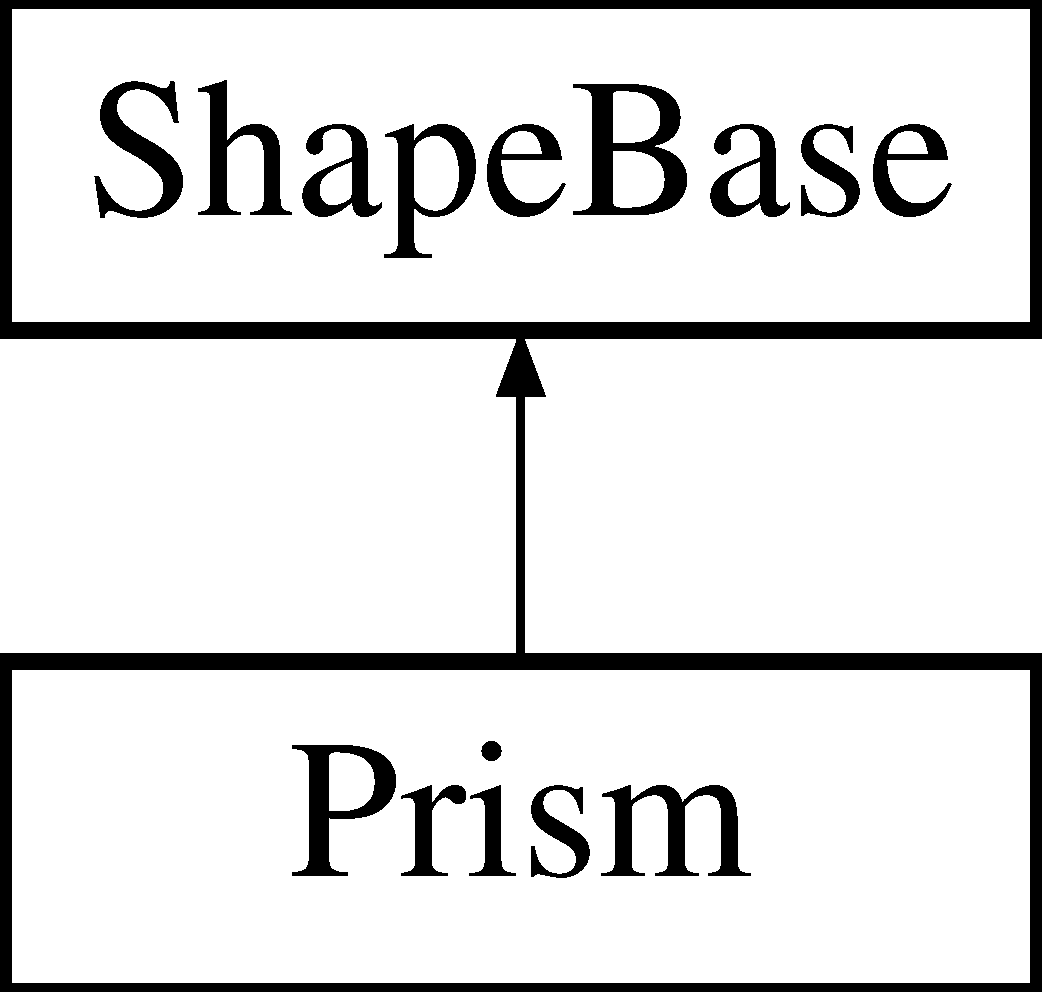
\includegraphics[height=2.000000cm]{classPrism}
\end{center}
\end{figure}
\subsection*{Public Member Functions}
\begin{DoxyCompactItemize}
\item 
\hypertarget{classPrism_aa107f8923cbbc9e1881cf98666743ae6}{}{\bfseries Prism} (int $\ast$Node\+Ids, vector$<$ \hyperlink{classNode}{Node} $\ast$ $>$ \&Nodes, int Curr\+Id)\label{classPrism_aa107f8923cbbc9e1881cf98666743ae6}

\item 
\hypertarget{classPrism_ab1eaaa559c1997fa7b30e84d7ce6b2d5}{}void {\bfseries set\+Elastic\+Properties} (double E\+Apical, double E\+Basal, double E\+Mid, double v)\label{classPrism_ab1eaaa559c1997fa7b30e84d7ce6b2d5}

\item 
\hypertarget{classPrism_aa65f89d72659c92de21c411a2fa23a7e}{}void {\bfseries calculate\+Basal\+Normal} (double $\ast$normal)\label{classPrism_aa65f89d72659c92de21c411a2fa23a7e}

\item 
\hypertarget{classPrism_a64100d877e59727ab9b7e9ad56e17cee}{}void {\bfseries Align\+Reference\+Base\+Normal\+To\+Z} ()\label{classPrism_a64100d877e59727ab9b7e9ad56e17cee}

\item 
\hypertarget{classPrism_a9a877cebf651015b88af641f1e045699}{}void {\bfseries calculate\+Element\+Shape\+Function\+Derivatives} ()\label{classPrism_a9a877cebf651015b88af641f1e045699}

\item 
\hypertarget{classPrism_af4ce210a9ba20d34b4b903e936b9dd8d}{}void {\bfseries check\+Health} ()\label{classPrism_af4ce210a9ba20d34b4b903e936b9dd8d}

\item 
\hypertarget{classPrism_ad9b04b2ad4cdedb878b4c7c0b4917a7a}{}void {\bfseries get\+Apical\+Triangles} (vector$<$ int $>$ \&Apical\+Triangles)\label{classPrism_ad9b04b2ad4cdedb878b4c7c0b4917a7a}

\item 
\hypertarget{classPrism_a10377e0ad0ae454a3cd25b82709119ac}{}int {\bfseries get\+Correcponding\+Apical} (int curr\+Node\+Id)\label{classPrism_a10377e0ad0ae454a3cd25b82709119ac}

\item 
\hypertarget{classPrism_abe648c5fa60635a50c14186135bed332}{}bool {\bfseries Is\+This\+Node\+My\+Basal} (int curr\+Node\+Id)\label{classPrism_abe648c5fa60635a50c14186135bed332}

\item 
\hypertarget{classPrism_a91d08cfcf6bf111f5d9e314499bafd11}{}double {\bfseries get\+Element\+Height} ()\label{classPrism_a91d08cfcf6bf111f5d9e314499bafd11}

\item 
\hypertarget{classPrism_aea2d84b05534bb2aedcdb49a53eab1ae}{}void {\bfseries Add\+Packing\+To\+Surface} (int tissueplacement\+Of\+Packing\+Node, double Fx, double Fy, double Fz, double $\ast$$\ast$Packing\+Forces, vector$<$ \hyperlink{classNode}{Node} $\ast$ $>$ \&Nodes, bool \&all\+Corners\+Fixed\+X, bool \&all\+Corners\+Fixed\+Y, bool \&all\+Corners\+Fixed\+Z)\label{classPrism_aea2d84b05534bb2aedcdb49a53eab1ae}

\item 
\hypertarget{classPrism_aa153c49304a9d808af5ea65a40f89128}{}void {\bfseries get\+Relevant\+Nodes\+For\+Packing} (int Tissue\+Placement\+Of\+Packing\+Node, int Tissue\+Type\+Of\+Packing\+Node, int \&id1, int \&id2, int \&id3)\label{classPrism_aa153c49304a9d808af5ea65a40f89128}

\item 
\hypertarget{classPrism_a45363ee4cc0dddd82ef567846a6bf123}{}bool {\bfseries Is\+Point\+Close\+Enough\+For\+Packing} (double $\ast$Pos, float threshold, int Tissue\+Placement\+Of\+Packing\+Node, int Tissue\+Type\+Of\+Packing\+Node)\label{classPrism_a45363ee4cc0dddd82ef567846a6bf123}

\item 
\hypertarget{classPrism_acb1603367b049392cebfc20b3aaeab87}{}void {\bfseries calculate\+Normal\+For\+Packing} (int tissue\+Placement\+Of\+Normal)\label{classPrism_acb1603367b049392cebfc20b3aaeab87}

\item 
\hypertarget{classPrism_a67e80515fb1cdf4438b4b7d47334bd2e}{}void {\bfseries calculate\+Apical\+Area} ()\label{classPrism_a67e80515fb1cdf4438b4b7d47334bd2e}

\item 
\hypertarget{classPrism_aa8dd4b90cdaecdbabfb48f45a9bcdc95}{}void {\bfseries calculate\+Basal\+Area} ()\label{classPrism_aa8dd4b90cdaecdbabfb48f45a9bcdc95}

\item 
\hypertarget{classPrism_a306261925defdb79ba64fc5f9ef8a23d}{}void {\bfseries calculate\+Myosin\+Forces} (double force\+Per\+Myo\+Molecule)\label{classPrism_a306261925defdb79ba64fc5f9ef8a23d}

\item 
\hypertarget{classPrism_ab11b5901fc7d65f71c7cccd1ce94a273}{}void {\bfseries distribute\+Myosin\+Force} (bool is\+Isotropic, bool apical, double force\+Per\+Myo\+Molecule)\label{classPrism_ab11b5901fc7d65f71c7cccd1ce94a273}

\item 
\hypertarget{classPrism_a243934a73a8f198ed592761ecb0927b9}{}void {\bfseries get\+Apical\+Node\+Pos} (double $\ast$pos\+Corner)\label{classPrism_a243934a73a8f198ed592761ecb0927b9}

\item 
\hypertarget{classPrism_a31324d23b37fa20911916ebb7ee1064d}{}void {\bfseries get\+Basal\+Node\+Pos} (double $\ast$pos\+Corner)\label{classPrism_a31324d23b37fa20911916ebb7ee1064d}

\item 
\hypertarget{classPrism_a26bb1eed04307a373ba87b48f1c1a3ca}{}bool {\bfseries Ispoint\+Inside\+Triangle} (int tissueplacement, double x, double y, double z)\label{classPrism_a26bb1eed04307a373ba87b48f1c1a3ca}

\item 
\hypertarget{classPrism_a85f9b472a3310e76ab0c76bd1fb7dd30}{}void {\bfseries check\+Rotation\+Consistency3\+D} ()\label{classPrism_a85f9b472a3310e76ab0c76bd1fb7dd30}

\end{DoxyCompactItemize}
\subsection*{Protected Member Functions}
\begin{DoxyCompactItemize}
\item 
\hypertarget{classPrism_a39d403ac6ffb6b56d5b2d07f8e9463a4}{}void {\bfseries set\+Tissue\+Coords\+Rotations\+Buffers} ()\label{classPrism_a39d403ac6ffb6b56d5b2d07f8e9463a4}

\item 
\hypertarget{classPrism_a3c252dc104a1ca7208b23c72737cd916}{}void {\bfseries get\+Curr\+Relaxed\+Shape} (gsl\+\_\+matrix $\ast$Curr\+Relaxed\+Shape)\label{classPrism_a3c252dc104a1ca7208b23c72737cd916}

\item 
\hypertarget{classPrism_aa1a4d3411d1f3dc05816ec01dcfa8310}{}void {\bfseries set\+Shape\+Function\+Derivatives} (gsl\+\_\+matrix $\ast$Shape\+Func\+Der, double eta, double zeta, double nu)\label{classPrism_aa1a4d3411d1f3dc05816ec01dcfa8310}

\item 
\hypertarget{classPrism_aa1f76f3cabdd00eb057f41cebbaa466d}{}void {\bfseries set\+Shape\+Function\+Derivative\+Stack} (gsl\+\_\+matrix $\ast$Shape\+Func\+Der, gsl\+\_\+matrix $\ast$Shape\+Func\+Der\+Stack)\label{classPrism_aa1f76f3cabdd00eb057f41cebbaa466d}

\item 
\hypertarget{classPrism_a0575442613f8b7d9428c58cef19ab219}{}void {\bfseries set\+Coeff\+Mat} ()\label{classPrism_a0575442613f8b7d9428c58cef19ab219}

\item 
\hypertarget{classPrism_aa433244f86cdf23a611a1adc3391c3f0}{}void {\bfseries calculate\+Currk} (boost\+::numeric\+::ublas\+::matrix$<$ double $>$ \&currk, boost\+::numeric\+::ublas\+::matrix$<$ double $>$ \&curr\+B, boost\+::numeric\+::ublas\+::matrix$<$ double $>$ \&curr\+B\+E, boost\+::numeric\+::ublas\+::matrix$<$ double $>$ \&curr\+Bo, double eta, double zeta, double nu)\label{classPrism_aa433244f86cdf23a611a1adc3391c3f0}

\item 
void \hyperlink{classPrism_a606fbf422f9d652e0f697ea93dc2e088}{calculate\+Curr\+Nodal\+Forces} (gsl\+\_\+matrix $\ast$gslcurrge, gsl\+\_\+matrix $\ast$gslcurrgv, gsl\+\_\+matrix $\ast$gslcurr\+F, gsl\+\_\+matrix $\ast$displacement\+Per\+Dt, int point\+No)
\item 
\hypertarget{classPrism_ae9403142a217a005a4d588a6e472be27}{}void {\bfseries calculate\+Curr\+Tri\+Point\+F\+For\+Rotation} (gsl\+\_\+matrix $\ast$curr\+F, int point\+No)\label{classPrism_ae9403142a217a005a4d588a6e472be27}

\item 
\hypertarget{classPrism_a872ce1e6304b1400d2d0e712af2a0131}{}void {\bfseries calculate\+Normal\+To\+Bottom} ()\label{classPrism_a872ce1e6304b1400d2d0e712af2a0131}

\item 
\hypertarget{classPrism_a2d8821dcd96009c95f06f34ee23ede7e}{}void {\bfseries calculate\+Reference\+Normal\+To\+Bottom} ()\label{classPrism_a2d8821dcd96009c95f06f34ee23ede7e}

\item 
\hypertarget{classPrism_ac3b85296d366eb4dd67406228c519caf}{}void {\bfseries calculate\+Normal\+To\+Top} ()\label{classPrism_ac3b85296d366eb4dd67406228c519caf}

\item 
\hypertarget{classPrism_a41a101de7bb2f75c5f9b44de23187593}{}void {\bfseries calculate\+Reference\+Normal\+To\+Top} ()\label{classPrism_a41a101de7bb2f75c5f9b44de23187593}

\item 
\hypertarget{classPrism_a6144314003601a688d81b0389ea1114e}{}void {\bfseries get\+Current\+Alignment\+Sides} (double $\ast$, double $\ast$)\label{classPrism_a6144314003601a688d81b0389ea1114e}

\item 
\hypertarget{classPrism_ab5fa417d944a6903b5bc9d2f53d4616a}{}void {\bfseries get\+Current\+Alignment\+Faces} (double $\ast$Ref\+Side, double $\ast$Shape\+Side, double $\ast$Ref\+Face, double $\ast$Shape\+Face)\label{classPrism_ab5fa417d944a6903b5bc9d2f53d4616a}

\item 
\hypertarget{classPrism_a4472375144e5e38a912af1fb4e2cc2d1}{}void {\bfseries update\+Alignment\+Turn} ()\label{classPrism_a4472375144e5e38a912af1fb4e2cc2d1}

\item 
\hypertarget{classPrism_a4ea58fd729a2bbef20530200978a8f75}{}void {\bfseries calculate\+Reference\+Volume} ()\label{classPrism_a4ea58fd729a2bbef20530200978a8f75}

\item 
\hypertarget{classPrism_a6b273d198e94039758a027b0dfb2c8af}{}void {\bfseries calculate\+Plane\+Normals} (double $\ast$$\ast$normals)\label{classPrism_a6b273d198e94039758a027b0dfb2c8af}

\item 
\hypertarget{classPrism_a13de4e8cefb58b3a33de4c2f7265a3b0}{}void {\bfseries assign\+Nodal\+Vector} (double $\ast$vec, int id0, int id1)\label{classPrism_a13de4e8cefb58b3a33de4c2f7265a3b0}

\item 
\hypertarget{classPrism_ac9695169749356654e847a022ce29aff}{}bool {\bfseries check\+Node\+Plane\+Consistency} (double $\ast$$\ast$normals)\label{classPrism_ac9695169749356654e847a022ce29aff}

\item 
\hypertarget{classPrism_acc59ccf5e1b5f459a8fb871c2a78fe8e}{}double {\bfseries get\+Apical\+Side\+Length\+Average} ()\label{classPrism_acc59ccf5e1b5f459a8fb871c2a78fe8e}

\end{DoxyCompactItemize}
\subsection*{Additional Inherited Members}


\subsection{Member Function Documentation}
\hypertarget{classPrism_a606fbf422f9d652e0f697ea93dc2e088}{}\index{Prism@{Prism}!calculate\+Curr\+Nodal\+Forces@{calculate\+Curr\+Nodal\+Forces}}
\index{calculate\+Curr\+Nodal\+Forces@{calculate\+Curr\+Nodal\+Forces}!Prism@{Prism}}
\subsubsection[{calculate\+Curr\+Nodal\+Forces}]{\setlength{\rightskip}{0pt plus 5cm}void Prism\+::calculate\+Curr\+Nodal\+Forces (
\begin{DoxyParamCaption}
\item[{gsl\+\_\+matrix $\ast$}]{gslcurrge, }
\item[{gsl\+\_\+matrix $\ast$}]{gslcurrgv, }
\item[{gsl\+\_\+matrix $\ast$}]{gslcurr\+F, }
\item[{gsl\+\_\+matrix $\ast$}]{displacement\+Per\+Dt, }
\item[{int}]{point\+No}
\end{DoxyParamCaption}
)\hspace{0.3cm}{\ttfamily [protected]}, {\ttfamily [virtual]}}\label{classPrism_a606fbf422f9d652e0f697ea93dc2e088}
$<$ Removing growth

$<$ Removing shape change

$<$ Removing shape change 

Reimplemented from \hyperlink{classShapeBase}{Shape\+Base}.



The documentation for this class was generated from the following files\+:\begin{DoxyCompactItemize}
\item 
/home/melda/\+Documents/\+Tissue\+Folding/\+Tissue\+Folding/\+Source\+Code/Prism.\+h\item 
/home/melda/\+Documents/\+Tissue\+Folding/\+Tissue\+Folding/\+Source\+Code/Prism.\+cpp\end{DoxyCompactItemize}

\hypertarget{classRandomGenerator}{}\section{Random\+Generator Class Reference}
\label{classRandomGenerator}\index{Random\+Generator@{Random\+Generator}}


{\ttfamily \#include $<$Random\+Generator.\+h$>$}

\subsection*{Public Member Functions}
\begin{DoxyCompactItemize}
\item 
\hyperlink{classRandomGenerator_ad2b3256e634878160c7d8b6e865341b2}{Random\+Generator} ()
\item 
vector$<$ double $>$ \hyperlink{classRandomGenerator_ade01887d86acde9c158dd3ee80250e47}{get\+Norm\+R\+V} (double mean, double var, unsigned int n)
\item 
double \hyperlink{classRandomGenerator_a96a04ffa03a3f0a3e95d50d7c7e828cb}{get\+Norm\+R\+V} (double mean, double var)
\item 
int \hyperlink{classRandomGenerator_a39a6365864741e8246546162b6e5a34e}{get\+Uniform\+R\+V} (int min, int max)
\item 
double \hyperlink{classRandomGenerator_ad584ae9751a4cd03b981ced9c12f4e6e}{get\+Uniform\+R\+V} (double min, double max)
\item 
std\+::string \hyperlink{classRandomGenerator_a2da3e84fb399d8af423547376a1aae42}{get\+Random\+Str} (unsigned int length)
\item 
void \hyperlink{classRandomGenerator_a35e84fa76d2bfaba05671aa0f79c1b0a}{Seed} ()
\end{DoxyCompactItemize}
\subsection*{Static Public Member Functions}
\begin{DoxyCompactItemize}
\item 
static \hyperlink{classRandomGenerator}{Random\+Generator} \& \hyperlink{classRandomGenerator_a6c161d5ba97abe160d46d031f2211eb7}{Obj} ()
\end{DoxyCompactItemize}


\subsection{Detailed Description}
The random number generator. 

\subsection{Constructor \& Destructor Documentation}
\hypertarget{classRandomGenerator_ad2b3256e634878160c7d8b6e865341b2}{}\index{Random\+Generator@{Random\+Generator}!Random\+Generator@{Random\+Generator}}
\index{Random\+Generator@{Random\+Generator}!Random\+Generator@{Random\+Generator}}
\subsubsection[{Random\+Generator}]{\setlength{\rightskip}{0pt plus 5cm}Random\+Generator\+::\+Random\+Generator (
\begin{DoxyParamCaption}
{}
\end{DoxyParamCaption}
)\hspace{0.3cm}{\ttfamily [inline]}}\label{classRandomGenerator_ad2b3256e634878160c7d8b6e865341b2}
Default constructor. 

\subsection{Member Function Documentation}
\hypertarget{classRandomGenerator_ade01887d86acde9c158dd3ee80250e47}{}\index{Random\+Generator@{Random\+Generator}!get\+Norm\+R\+V@{get\+Norm\+R\+V}}
\index{get\+Norm\+R\+V@{get\+Norm\+R\+V}!Random\+Generator@{Random\+Generator}}
\subsubsection[{get\+Norm\+R\+V}]{\setlength{\rightskip}{0pt plus 5cm}vector$<$double$>$ Random\+Generator\+::get\+Norm\+R\+V (
\begin{DoxyParamCaption}
\item[{double}]{mean, }
\item[{double}]{var, }
\item[{unsigned int}]{n}
\end{DoxyParamCaption}
)\hspace{0.3cm}{\ttfamily [inline]}}\label{classRandomGenerator_ade01887d86acde9c158dd3ee80250e47}
Get a given number of normally-\/distributed random variables. \hypertarget{classRandomGenerator_a96a04ffa03a3f0a3e95d50d7c7e828cb}{}\index{Random\+Generator@{Random\+Generator}!get\+Norm\+R\+V@{get\+Norm\+R\+V}}
\index{get\+Norm\+R\+V@{get\+Norm\+R\+V}!Random\+Generator@{Random\+Generator}}
\subsubsection[{get\+Norm\+R\+V}]{\setlength{\rightskip}{0pt plus 5cm}double Random\+Generator\+::get\+Norm\+R\+V (
\begin{DoxyParamCaption}
\item[{double}]{mean, }
\item[{double}]{var}
\end{DoxyParamCaption}
)\hspace{0.3cm}{\ttfamily [inline]}}\label{classRandomGenerator_a96a04ffa03a3f0a3e95d50d7c7e828cb}
Get a normally-\/distributed random variable. \hypertarget{classRandomGenerator_a2da3e84fb399d8af423547376a1aae42}{}\index{Random\+Generator@{Random\+Generator}!get\+Random\+Str@{get\+Random\+Str}}
\index{get\+Random\+Str@{get\+Random\+Str}!Random\+Generator@{Random\+Generator}}
\subsubsection[{get\+Random\+Str}]{\setlength{\rightskip}{0pt plus 5cm}std\+::string Random\+Generator\+::get\+Random\+Str (
\begin{DoxyParamCaption}
\item[{unsigned int}]{length}
\end{DoxyParamCaption}
)\hspace{0.3cm}{\ttfamily [inline]}}\label{classRandomGenerator_a2da3e84fb399d8af423547376a1aae42}
Get a randomised string of a certain length. \hypertarget{classRandomGenerator_a39a6365864741e8246546162b6e5a34e}{}\index{Random\+Generator@{Random\+Generator}!get\+Uniform\+R\+V@{get\+Uniform\+R\+V}}
\index{get\+Uniform\+R\+V@{get\+Uniform\+R\+V}!Random\+Generator@{Random\+Generator}}
\subsubsection[{get\+Uniform\+R\+V}]{\setlength{\rightskip}{0pt plus 5cm}int Random\+Generator\+::get\+Uniform\+R\+V (
\begin{DoxyParamCaption}
\item[{int}]{min, }
\item[{int}]{max}
\end{DoxyParamCaption}
)\hspace{0.3cm}{\ttfamily [inline]}}\label{classRandomGenerator_a39a6365864741e8246546162b6e5a34e}
Get a uniformly distributed R\+V in \mbox{[}m,n\mbox{]} (m,n are int). \hypertarget{classRandomGenerator_ad584ae9751a4cd03b981ced9c12f4e6e}{}\index{Random\+Generator@{Random\+Generator}!get\+Uniform\+R\+V@{get\+Uniform\+R\+V}}
\index{get\+Uniform\+R\+V@{get\+Uniform\+R\+V}!Random\+Generator@{Random\+Generator}}
\subsubsection[{get\+Uniform\+R\+V}]{\setlength{\rightskip}{0pt plus 5cm}double Random\+Generator\+::get\+Uniform\+R\+V (
\begin{DoxyParamCaption}
\item[{double}]{min, }
\item[{double}]{max}
\end{DoxyParamCaption}
)\hspace{0.3cm}{\ttfamily [inline]}}\label{classRandomGenerator_ad584ae9751a4cd03b981ced9c12f4e6e}
Get a uniformly distributed R\+V in \mbox{[}m,n\mbox{]} (m,n are int). \hypertarget{classRandomGenerator_a6c161d5ba97abe160d46d031f2211eb7}{}\index{Random\+Generator@{Random\+Generator}!Obj@{Obj}}
\index{Obj@{Obj}!Random\+Generator@{Random\+Generator}}
\subsubsection[{Obj}]{\setlength{\rightskip}{0pt plus 5cm}static {\bf Random\+Generator}\& Random\+Generator\+::\+Obj (
\begin{DoxyParamCaption}
{}
\end{DoxyParamCaption}
)\hspace{0.3cm}{\ttfamily [inline]}, {\ttfamily [static]}}\label{classRandomGenerator_a6c161d5ba97abe160d46d031f2211eb7}
The random generator access function. \hypertarget{classRandomGenerator_a35e84fa76d2bfaba05671aa0f79c1b0a}{}\index{Random\+Generator@{Random\+Generator}!Seed@{Seed}}
\index{Seed@{Seed}!Random\+Generator@{Random\+Generator}}
\subsubsection[{Seed}]{\setlength{\rightskip}{0pt plus 5cm}void Random\+Generator\+::\+Seed (
\begin{DoxyParamCaption}
{}
\end{DoxyParamCaption}
)\hspace{0.3cm}{\ttfamily [inline]}}\label{classRandomGenerator_a35e84fa76d2bfaba05671aa0f79c1b0a}
Seed the generator. 

The documentation for this class was generated from the following files\+:\begin{DoxyCompactItemize}
\item 
/home/melda/\+Documents/\+Tissue\+Folding/\+Tissue\+Folding/\+Source\+Code/Random\+Generator.\+h\item 
/home/melda/\+Documents/\+Tissue\+Folding/\+Tissue\+Folding/\+Source\+Code/Random\+Generator.\+cpp\end{DoxyCompactItemize}

\hypertarget{classReferenceShapeBase}{}\section{Reference\+Shape\+Base Class Reference}
\label{classReferenceShapeBase}\index{Reference\+Shape\+Base@{Reference\+Shape\+Base}}
\subsection*{Public Member Functions}
\begin{DoxyCompactItemize}
\item 
\hypertarget{classReferenceShapeBase_a3d27b5bf4c591a5973b466d2af08a118}{}\hyperlink{classReferenceShapeBase_a3d27b5bf4c591a5973b466d2af08a118}{Reference\+Shape\+Base} (string Syape\+Type, int \hyperlink{classReferenceShapeBase_af0da93cee3f17800d7aa90b21b1b81c7}{Id})\label{classReferenceShapeBase_a3d27b5bf4c591a5973b466d2af08a118}

\begin{DoxyCompactList}\small\item\em Constructer of the \hyperlink{classReferenceShapeBase}{Reference\+Shape\+Base} class. \end{DoxyCompactList}\item 
\hypertarget{classReferenceShapeBase_addf60ebee57a9d3b0e345b963901e3b5}{}\hyperlink{classReferenceShapeBase_addf60ebee57a9d3b0e345b963901e3b5}{$\sim$\+Reference\+Shape\+Base} ()\label{classReferenceShapeBase_addf60ebee57a9d3b0e345b963901e3b5}

\begin{DoxyCompactList}\small\item\em Destructor of the \hyperlink{classReferenceShapeBase}{Reference\+Shape\+Base} class. \end{DoxyCompactList}\end{DoxyCompactItemize}
\subsection*{Public Attributes}
\begin{DoxyCompactItemize}
\item 
\hypertarget{classReferenceShapeBase_a745e71ff73ef758708f39a4b3b1be4d1}{}double $\ast$$\ast$ \hyperlink{classReferenceShapeBase_a745e71ff73ef758708f39a4b3b1be4d1}{Positions}\label{classReferenceShapeBase_a745e71ff73ef758708f39a4b3b1be4d1}

\begin{DoxyCompactList}\small\item\em The pointer to the position matrix of the reference element. The array itself is declared within the constructor, depending on \hyperlink{classShapeBase_a250bd3396546342c8104f5b9c180d18f}{Shape\+Base\+::n\+Dim} and \hyperlink{classShapeBase_ae7dd93b58b3281ce90025f83d0f0e976}{Shape\+Base\+::n\+Nodes}, its size being \mbox{[}n\+Nodes\mbox{]}\mbox{[}n\+Dim\mbox{]}. \end{DoxyCompactList}\item 
\hypertarget{classReferenceShapeBase_a12d2d0c2511f4f1357360ff61910ac02}{}double \hyperlink{classReferenceShapeBase_a12d2d0c2511f4f1357360ff61910ac02}{Volume}\label{classReferenceShapeBase_a12d2d0c2511f4f1357360ff61910ac02}

\begin{DoxyCompactList}\small\item\em The volume of reference element, calculated assuming regular shapes (e.\+g. Perpendicular prism of equal top and bottom surfaces). \end{DoxyCompactList}\item 
\hypertarget{classReferenceShapeBase_a214b89b970efa7a290dbe1533cf237ea}{}double \hyperlink{classReferenceShapeBase_a214b89b970efa7a290dbe1533cf237ea}{Basal\+Area}\label{classReferenceShapeBase_a214b89b970efa7a290dbe1533cf237ea}

\begin{DoxyCompactList}\small\item\em The basal area of the reference shape. \end{DoxyCompactList}\item 
\hypertarget{classReferenceShapeBase_a76ac694d1b1276f6847bee3c3efa84b0}{}double \hyperlink{classReferenceShapeBase_a76ac694d1b1276f6847bee3c3efa84b0}{height}\label{classReferenceShapeBase_a76ac694d1b1276f6847bee3c3efa84b0}

\begin{DoxyCompactList}\small\item\em Slab height for 2\+D elements, value is -\/100 for 3\+D elements. Is obsolete now, must be deleted together with any 2\+D element option. Mesh file reading should be cleared in parallel. \end{DoxyCompactList}\end{DoxyCompactItemize}
\subsection*{Protected Member Functions}
\begin{DoxyCompactItemize}
\item 
\hypertarget{classReferenceShapeBase_ad893cb0986899d77de34ce5e565ebb97}{}void {\bfseries set\+Shape\+Type} (string Type\+Name)\label{classReferenceShapeBase_ad893cb0986899d77de34ce5e565ebb97}

\item 
\hypertarget{classReferenceShapeBase_a027db08b5e580286448380aa21902b33}{}void {\bfseries set\+Node\+Number} ()\label{classReferenceShapeBase_a027db08b5e580286448380aa21902b33}

\end{DoxyCompactItemize}
\subsection*{Protected Attributes}
\begin{DoxyCompactItemize}
\item 
\hypertarget{classReferenceShapeBase_a4831a54cffbafef4ded26fb8c50566e0}{}int \hyperlink{classReferenceShapeBase_a4831a54cffbafef4ded26fb8c50566e0}{Shape\+Type}\label{classReferenceShapeBase_a4831a54cffbafef4ded26fb8c50566e0}

\begin{DoxyCompactList}\small\item\em The integer defining the type of the shape, it is a negative value at the same basis of \hyperlink{classShapeBase_a36aedd41e8465a186a0b0c454b5b76f3}{Shape\+Base\+::\+Shape\+Type}\+: prisms Shape\+Type = -\/1. \end{DoxyCompactList}\item 
\hypertarget{classReferenceShapeBase_af0da93cee3f17800d7aa90b21b1b81c7}{}int \hyperlink{classReferenceShapeBase_af0da93cee3f17800d7aa90b21b1b81c7}{Id}\label{classReferenceShapeBase_af0da93cee3f17800d7aa90b21b1b81c7}

\begin{DoxyCompactList}\small\item\em The unique identifier of the reference shape, it is identical to the owner shape, it is set inside the constructor. \end{DoxyCompactList}\item 
\hypertarget{classReferenceShapeBase_a1183c092056a3245a350ff6f56632633}{}int \hyperlink{classReferenceShapeBase_a1183c092056a3245a350ff6f56632633}{n\+Nodes}\label{classReferenceShapeBase_a1183c092056a3245a350ff6f56632633}

\begin{DoxyCompactList}\small\item\em The number of nodes of the reference element, it is based on \hyperlink{classReferenceShapeBase_a4831a54cffbafef4ded26fb8c50566e0}{Reference\+Shape\+Base\+::\+Shape\+Type}, through function Reference\+Shape\+Base\+::set\+Node\+Number. \end{DoxyCompactList}\end{DoxyCompactItemize}


The documentation for this class was generated from the following files\+:\begin{DoxyCompactItemize}
\item 
/home/melda/\+Documents/\+Tissue\+Folding/\+Tissue\+Folding/\+Source\+Code/Reference\+Shape\+Base.\+h\item 
/home/melda/\+Documents/\+Tissue\+Folding/\+Tissue\+Folding/\+Source\+Code/Reference\+Shape\+Base.\+cpp\end{DoxyCompactItemize}

\hypertarget{classRingGrowthFunction}{}\section{Ring\+Growth\+Function Class Reference}
\label{classRingGrowthFunction}\index{Ring\+Growth\+Function@{Ring\+Growth\+Function}}
Inheritance diagram for Ring\+Growth\+Function\+:\begin{figure}[H]
\begin{center}
\leavevmode
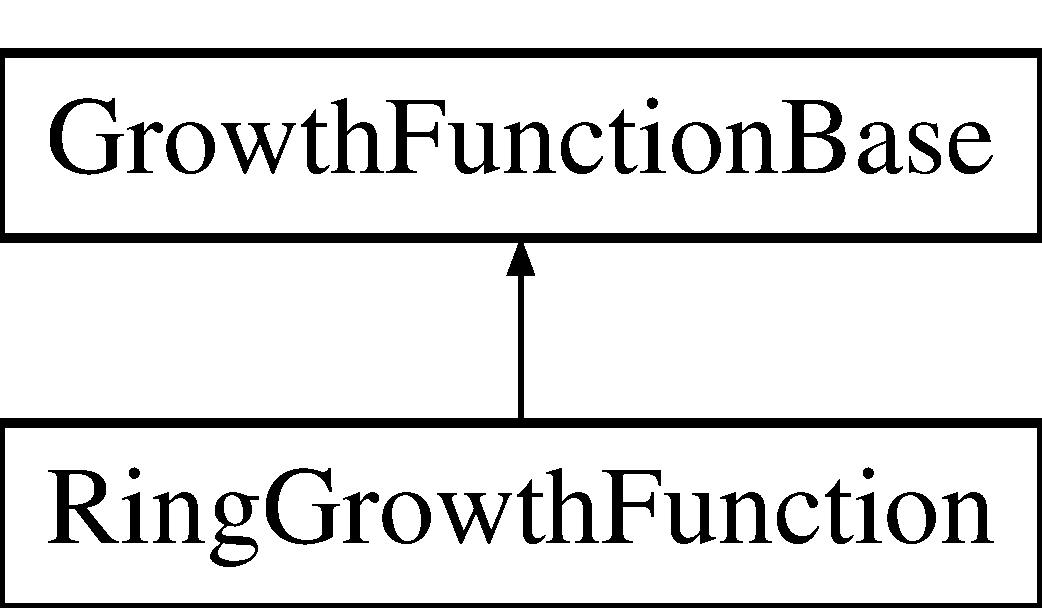
\includegraphics[height=2.000000cm]{classRingGrowthFunction}
\end{center}
\end{figure}
\subsection*{Public Member Functions}
\begin{DoxyCompactItemize}
\item 
\hyperlink{classRingGrowthFunction_a2e12b527d77b74130258ad25dc18e88d}{Ring\+Growth\+Function} (int id, int type, float \hyperlink{classGrowthFunctionBase_ae92513a7b41637df8e26e7db35ddf97c}{init\+Time}, float \hyperlink{classGrowthFunctionBase_a3ff4db0573d354a75666a5f3ca446941}{end\+Time}, bool \hyperlink{classGrowthFunctionBase_a3d56771e7c145589a14e11cc331e0326}{apply\+To\+Columnar\+Layer}, bool \hyperlink{classGrowthFunctionBase_a08ae19f58cb98fa8e315a77f52749732}{apply\+To\+Peripodial\+Membrane}, double Cx, double Cy, double inner\+R, double outer\+R, double D\+V\+Growth, double A\+P\+Growth, double A\+B\+Growth, double \hyperlink{classRingGrowthFunction_add6283d1ad999925c4202a3fa66b76ea}{angle})
\begin{DoxyCompactList}\small\item\em The constructor of \hyperlink{classRingGrowthFunction}{Ring\+Growth\+Function}. \end{DoxyCompactList}\item 
\hypertarget{classRingGrowthFunction_aa2063170e3ee5c5f22d7beef32300e9c}{}void \hyperlink{classRingGrowthFunction_aa2063170e3ee5c5f22d7beef32300e9c}{get\+Centre} (float \&centre\+X, float \&centre\+Y)\label{classRingGrowthFunction_aa2063170e3ee5c5f22d7beef32300e9c}

\begin{DoxyCompactList}\small\item\em This function writes \hyperlink{classRingGrowthFunction_a5b8f1cc72d03907bb1492e6c2f288db0}{Ring\+Growth\+Function\+::centre} into the input float addresses centre\+X and centre\+Y, in this order. \end{DoxyCompactList}\item 
\hypertarget{classRingGrowthFunction_ae1f4f4cecfab3ec343c748cfe78ab70b}{}float \hyperlink{classRingGrowthFunction_ae1f4f4cecfab3ec343c748cfe78ab70b}{get\+Inner\+Radius} ()\label{classRingGrowthFunction_ae1f4f4cecfab3ec343c748cfe78ab70b}

\begin{DoxyCompactList}\small\item\em This function returns \hyperlink{classRingGrowthFunction_a4e8796fbbbe9fe18c2dcd04613effcf0}{Ring\+Growth\+Function\+::inner\+Radius}. \end{DoxyCompactList}\item 
\hypertarget{classRingGrowthFunction_ad5c890c72a8ce520411d28e929faec19}{}float \hyperlink{classRingGrowthFunction_ad5c890c72a8ce520411d28e929faec19}{get\+Outer\+Radius} ()\label{classRingGrowthFunction_ad5c890c72a8ce520411d28e929faec19}

\begin{DoxyCompactList}\small\item\em This function returns \hyperlink{classRingGrowthFunction_a8b7d5268d9d47f112b56feef58193649}{Ring\+Growth\+Function\+::outer\+Radius}. \end{DoxyCompactList}\item 
void \hyperlink{classRingGrowthFunction_ab3cc1858fb602ab40a74af7d0467c13b}{get\+Growth\+Rate} (double $\ast$max\+Values)
\begin{DoxyCompactList}\small\item\em The function is to set the 3\+D maximum growth rate of the current ring growth function. \end{DoxyCompactList}\item 
void \hyperlink{classRingGrowthFunction_a051da280e649c81afff38a1a45cb035a}{set\+Growt\+Rate} (double ex, double ey, double ez)
\begin{DoxyCompactList}\small\item\em The function is to set the 3\+D maximum growth rate of the current ring growth function. \end{DoxyCompactList}\item 
\hypertarget{classRingGrowthFunction_a05f880ba6df8b3001a8e8fdec5ba1ad6}{}gsl\+\_\+matrix $\ast$ \hyperlink{classRingGrowthFunction_a05f880ba6df8b3001a8e8fdec5ba1ad6}{get\+Shear\+Angle\+Rotation\+Matrix} ()\label{classRingGrowthFunction_a05f880ba6df8b3001a8e8fdec5ba1ad6}

\begin{DoxyCompactList}\small\item\em The function return the matrix pointer to the oriented growth rotation matrix. \end{DoxyCompactList}\item 
\hypertarget{classRingGrowthFunction_aa70523c66dce48e7e54360596787a629}{}double \hyperlink{classRingGrowthFunction_aa70523c66dce48e7e54360596787a629}{get\+Shear\+Angle} ()\label{classRingGrowthFunction_aa70523c66dce48e7e54360596787a629}

\begin{DoxyCompactList}\small\item\em The function returns the oriented growth angle in radians (double). \end{DoxyCompactList}\item 
void \hyperlink{classRingGrowthFunction_a681175045cf09fadd92921e129737e65}{write\+Summary} (ofstream \&save\+File\+Simulation\+Summary, double dt)
\begin{DoxyCompactList}\small\item\em The function is to write the growth function summary to simulation summary file. \end{DoxyCompactList}\end{DoxyCompactItemize}
\subsection*{Public Attributes}
\begin{DoxyCompactItemize}
\item 
\hypertarget{classRingGrowthFunction_a5b8f1cc72d03907bb1492e6c2f288db0}{}double \hyperlink{classRingGrowthFunction_a5b8f1cc72d03907bb1492e6c2f288db0}{centre} \mbox{[}2\mbox{]}\label{classRingGrowthFunction_a5b8f1cc72d03907bb1492e6c2f288db0}

\begin{DoxyCompactList}\small\item\em The double array of 2, giving the centre of the ring in micro-\/meters, format \mbox{[}x, y\mbox{]}. \end{DoxyCompactList}\item 
\hypertarget{classRingGrowthFunction_a4e8796fbbbe9fe18c2dcd04613effcf0}{}double \hyperlink{classRingGrowthFunction_a4e8796fbbbe9fe18c2dcd04613effcf0}{inner\+Radius}\label{classRingGrowthFunction_a4e8796fbbbe9fe18c2dcd04613effcf0}

\begin{DoxyCompactList}\small\item\em The inner radius of the ring, inner boundary of the growth region in micro-\/meters. The growth will be zero at and inside the inner radius. This value can be set to zero to have circular growth. \end{DoxyCompactList}\item 
\hypertarget{classRingGrowthFunction_a8b7d5268d9d47f112b56feef58193649}{}double \hyperlink{classRingGrowthFunction_a8b7d5268d9d47f112b56feef58193649}{outer\+Radius}\label{classRingGrowthFunction_a8b7d5268d9d47f112b56feef58193649}

\begin{DoxyCompactList}\small\item\em The outer radius of the ring, outer boundary of the growth region in micro-\/meters. The growth will be at the maximum value set by \hyperlink{classRingGrowthFunction_a93b70ff6a7258c73a6bd2d888d09fc09}{Ring\+Growth\+Function\+::\+Growth\+Rate} at the outer radius. \end{DoxyCompactList}\item 
\hypertarget{classRingGrowthFunction_a93b70ff6a7258c73a6bd2d888d09fc09}{}double \hyperlink{classRingGrowthFunction_a93b70ff6a7258c73a6bd2d888d09fc09}{Growth\+Rate} \mbox{[}3\mbox{]}\label{classRingGrowthFunction_a93b70ff6a7258c73a6bd2d888d09fc09}

\begin{DoxyCompactList}\small\item\em The maximum growth rate at the \hyperlink{classRingGrowthFunction_a8b7d5268d9d47f112b56feef58193649}{Ring\+Growth\+Function\+::outer\+Radius}, in (1/sec), format\+: \mbox{[} D\+V axis (x), A\+P axis (y), and A\+B axis (z)\mbox{]}. \end{DoxyCompactList}\item 
\hypertarget{classRingGrowthFunction_a9603e5de21f7bca0c23deff2c1e9efd6}{}gsl\+\_\+matrix $\ast$ \hyperlink{classRingGrowthFunction_a9603e5de21f7bca0c23deff2c1e9efd6}{Shear\+Angle\+Rotation\+Matrix}\label{classRingGrowthFunction_a9603e5de21f7bca0c23deff2c1e9efd6}

\begin{DoxyCompactList}\small\item\em The rotation matrix for the orientation of the growth on x-\/y plane. This matrix is constructed through \hyperlink{classUniformGrowthFunction_a1a985ff52f9796688e00942b4d3349f8}{Uniform\+Growth\+Function\+::angle}. \end{DoxyCompactList}\item 
\hypertarget{classRingGrowthFunction_add6283d1ad999925c4202a3fa66b76ea}{}double \hyperlink{classRingGrowthFunction_add6283d1ad999925c4202a3fa66b76ea}{angle}\label{classRingGrowthFunction_add6283d1ad999925c4202a3fa66b76ea}

\begin{DoxyCompactList}\small\item\em The rotation angle for the orientation of the growth on x-\/y plane. \end{DoxyCompactList}\end{DoxyCompactItemize}


\subsection{Constructor \& Destructor Documentation}
\hypertarget{classRingGrowthFunction_a2e12b527d77b74130258ad25dc18e88d}{}\index{Ring\+Growth\+Function@{Ring\+Growth\+Function}!Ring\+Growth\+Function@{Ring\+Growth\+Function}}
\index{Ring\+Growth\+Function@{Ring\+Growth\+Function}!Ring\+Growth\+Function@{Ring\+Growth\+Function}}
\subsubsection[{Ring\+Growth\+Function}]{\setlength{\rightskip}{0pt plus 5cm}Ring\+Growth\+Function\+::\+Ring\+Growth\+Function (
\begin{DoxyParamCaption}
\item[{int}]{id, }
\item[{int}]{type, }
\item[{float}]{init\+Time, }
\item[{float}]{end\+Time, }
\item[{bool}]{apply\+To\+Columnar\+Layer, }
\item[{bool}]{apply\+To\+Peripodial\+Membrane, }
\item[{double}]{Cx, }
\item[{double}]{Cy, }
\item[{double}]{inner\+R, }
\item[{double}]{outer\+R, }
\item[{double}]{D\+V\+Growth, }
\item[{double}]{A\+P\+Growth, }
\item[{double}]{A\+B\+Growth, }
\item[{double}]{angle}
\end{DoxyParamCaption}
)\hspace{0.3cm}{\ttfamily [inline]}}\label{classRingGrowthFunction_a2e12b527d77b74130258ad25dc18e88d}


The constructor of \hyperlink{classRingGrowthFunction}{Ring\+Growth\+Function}. 

The first six parameters will be directed to the parent constructor, \hyperlink{classGrowthFunctionBase_a061b31ad8a0cb228628c7104029a94bf}{Growth\+Function\+Base\+::\+Growth\+Function\+Base}. ~\newline
doubles Cx and Cy will set \hyperlink{classRingGrowthFunction_a5b8f1cc72d03907bb1492e6c2f288db0}{Ring\+Growth\+Function\+::centre}\mbox{[}0\mbox{]} and \hyperlink{classRingGrowthFunction_a5b8f1cc72d03907bb1492e6c2f288db0}{Ring\+Growth\+Function\+::centre}\mbox{[}1\mbox{]}, respectively. ~\newline
doubles inner\+R and outer\+R will set \hyperlink{classRingGrowthFunction_a4e8796fbbbe9fe18c2dcd04613effcf0}{Ring\+Growth\+Function\+::inner\+Radius} and \hyperlink{classRingGrowthFunction_a8b7d5268d9d47f112b56feef58193649}{Ring\+Growth\+Function\+::outer\+Radius}, respectively. ~\newline
doubles D\+V\+Growth, A\+P\+Growth and A\+B\+Growth will set the \hyperlink{classRingGrowthFunction_a93b70ff6a7258c73a6bd2d888d09fc09}{Ring\+Growth\+Function\+::\+Growth\+Rate}, in the given order.

\subsection{Member Function Documentation}
\hypertarget{classRingGrowthFunction_ab3cc1858fb602ab40a74af7d0467c13b}{}\index{Ring\+Growth\+Function@{Ring\+Growth\+Function}!get\+Growth\+Rate@{get\+Growth\+Rate}}
\index{get\+Growth\+Rate@{get\+Growth\+Rate}!Ring\+Growth\+Function@{Ring\+Growth\+Function}}
\subsubsection[{get\+Growth\+Rate}]{\setlength{\rightskip}{0pt plus 5cm}void Ring\+Growth\+Function\+::get\+Growth\+Rate (
\begin{DoxyParamCaption}
\item[{double $\ast$}]{max\+Values}
\end{DoxyParamCaption}
)\hspace{0.3cm}{\ttfamily [inline]}, {\ttfamily [virtual]}}\label{classRingGrowthFunction_ab3cc1858fb602ab40a74af7d0467c13b}


The function is to set the 3\+D maximum growth rate of the current ring growth function. 

This function will write the \hyperlink{classRingGrowthFunction_a93b70ff6a7258c73a6bd2d888d09fc09}{Ring\+Growth\+Function\+::\+Growth\+Rate} of the current growth function to the input double array pointer. The double array pointer should be set to point at a double array of size 3 (or higher) before calling the function.

Reimplemented from \hyperlink{classGrowthFunctionBase}{Growth\+Function\+Base}.

\hypertarget{classRingGrowthFunction_a051da280e649c81afff38a1a45cb035a}{}\index{Ring\+Growth\+Function@{Ring\+Growth\+Function}!set\+Growt\+Rate@{set\+Growt\+Rate}}
\index{set\+Growt\+Rate@{set\+Growt\+Rate}!Ring\+Growth\+Function@{Ring\+Growth\+Function}}
\subsubsection[{set\+Growt\+Rate}]{\setlength{\rightskip}{0pt plus 5cm}void Ring\+Growth\+Function\+::set\+Growt\+Rate (
\begin{DoxyParamCaption}
\item[{double}]{ex, }
\item[{double}]{ey, }
\item[{double}]{ez}
\end{DoxyParamCaption}
)\hspace{0.3cm}{\ttfamily [inline]}, {\ttfamily [virtual]}}\label{classRingGrowthFunction_a051da280e649c81afff38a1a45cb035a}


The function is to set the 3\+D maximum growth rate of the current ring growth function. 

This function will set the \hyperlink{classRingGrowthFunction_a93b70ff6a7258c73a6bd2d888d09fc09}{Ring\+Growth\+Function\+::\+Growth\+Rate} of the current growth function to the input values The parameters are in the order \mbox{[} D\+V axis (x), A\+P axis (y), and A\+B axis (z)\mbox{]}.

Reimplemented from \hyperlink{classGrowthFunctionBase}{Growth\+Function\+Base}.

\hypertarget{classRingGrowthFunction_a681175045cf09fadd92921e129737e65}{}\index{Ring\+Growth\+Function@{Ring\+Growth\+Function}!write\+Summary@{write\+Summary}}
\index{write\+Summary@{write\+Summary}!Ring\+Growth\+Function@{Ring\+Growth\+Function}}
\subsubsection[{write\+Summary}]{\setlength{\rightskip}{0pt plus 5cm}void Ring\+Growth\+Function\+::write\+Summary (
\begin{DoxyParamCaption}
\item[{ofstream \&}]{save\+File\+Simulation\+Summary, }
\item[{double}]{dt}
\end{DoxyParamCaption}
)\hspace{0.3cm}{\ttfamily [inline]}, {\ttfamily [virtual]}}\label{classRingGrowthFunction_a681175045cf09fadd92921e129737e65}


The function is to write the growth function summary to simulation summary file. 

This function will write the \hyperlink{classRingGrowthFunction}{Ring\+Growth\+Function} details into the simulation summary file, provided as the first input. Time step (dt) of the simulation is provided as second input, to report the growth rates per hour. The output should look like\+: ~\newline
 Growth Type\+: Ring (2) Initial time(sec)\+: \hyperlink{classGrowthFunctionBase_ae92513a7b41637df8e26e7db35ddf97c}{Ring\+Growth\+Function\+::init\+Time} Final\+Time time(sec)\+: \hyperlink{classGrowthFunctionBase_a3ff4db0573d354a75666a5f3ca446941}{Ring\+Growth\+Function\+::end\+Time} Centre(micron)\+: \hyperlink{classRingGrowthFunction_a5b8f1cc72d03907bb1492e6c2f288db0}{Ring\+Growth\+Function\+::centre}\mbox{[}0\mbox{]} \hyperlink{classRingGrowthFunction_a5b8f1cc72d03907bb1492e6c2f288db0}{Ring\+Growth\+Function\+::centre}\mbox{[}1\mbox{]} Inner radius(micron)\+: \hyperlink{classRingGrowthFunction_a4e8796fbbbe9fe18c2dcd04613effcf0}{Ring\+Growth\+Function\+::inner\+Radius} Outer radius(micron)\+: \hyperlink{classRingGrowthFunction_a8b7d5268d9d47f112b56feef58193649}{Ring\+Growth\+Function\+::outer\+Radius} Growth\+Rate(fraction/hr)\+:D\+V\+Growth(in 1/hr) A\+P\+Growth(in 1/hr) A\+B\+Growth(in 1/hr)

Reimplemented from \hyperlink{classGrowthFunctionBase}{Growth\+Function\+Base}.



The documentation for this class was generated from the following file\+:\begin{DoxyCompactItemize}
\item 
/home/melda/\+Documents/\+Tissue\+Folding/\+Tissue\+Folding/\+Source\+Code/Growth\+Function\+Types.\+h\end{DoxyCompactItemize}

\hypertarget{classShapeBase}{}\section{Shape\+Base Class Reference}
\label{classShapeBase}\index{Shape\+Base@{Shape\+Base}}
Inheritance diagram for Shape\+Base\+:\begin{figure}[H]
\begin{center}
\leavevmode
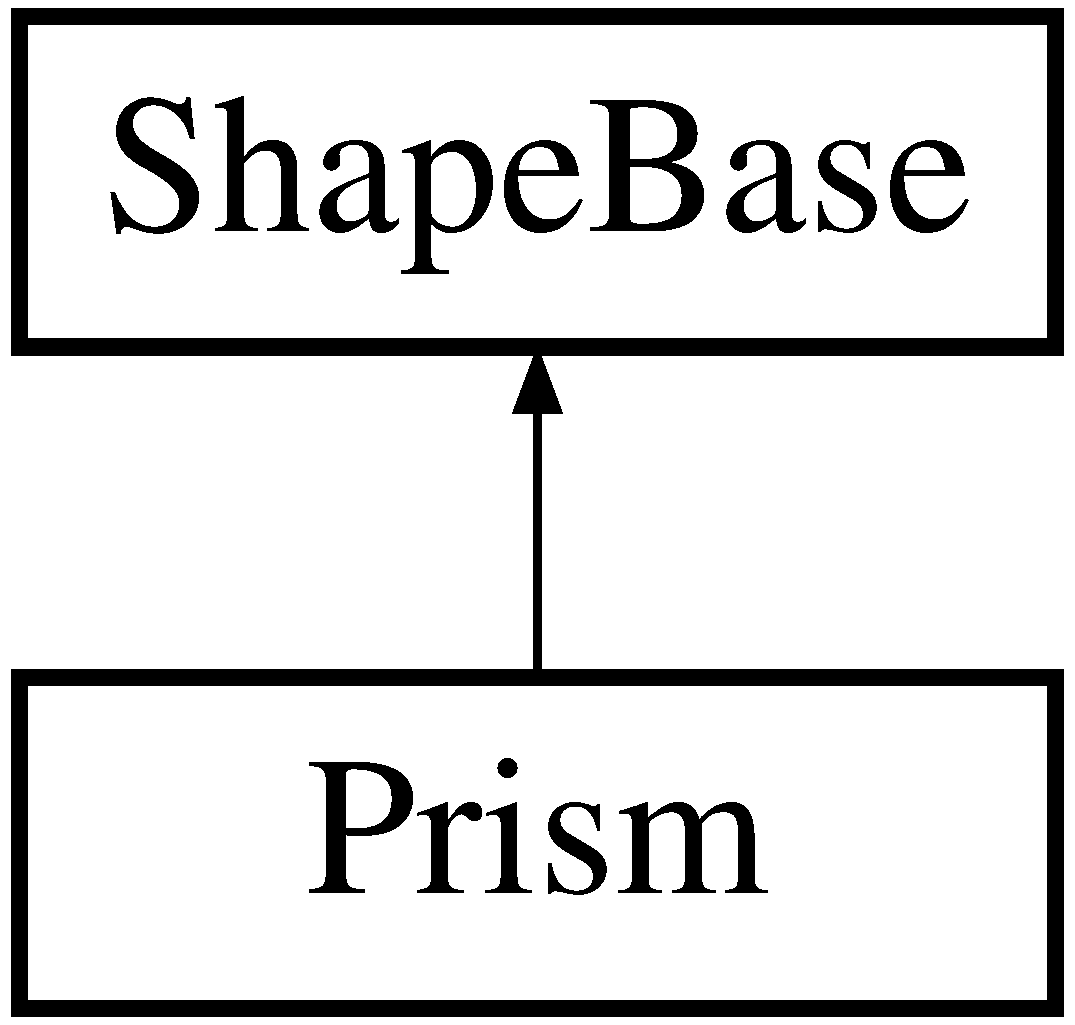
\includegraphics[height=2.000000cm]{classShapeBase}
\end{center}
\end{figure}
\subsection*{Public Member Functions}
\begin{DoxyCompactItemize}
\item 
\hypertarget{classShapeBase_ab55ac0089ea8e37649b0d85409c008ac}{}int {\bfseries get\+Id} ()\label{classShapeBase_ab55ac0089ea8e37649b0d85409c008ac}

\item 
\hypertarget{classShapeBase_a49d134532a98fb0cecacec44baf2baf3}{}string {\bfseries get\+Name} ()\label{classShapeBase_a49d134532a98fb0cecacec44baf2baf3}

\item 
\hypertarget{classShapeBase_a7ae6deee4256eb19c6e99b52a40847cb}{}int {\bfseries get\+Shape\+Type} ()\label{classShapeBase_a7ae6deee4256eb19c6e99b52a40847cb}

\item 
\hypertarget{classShapeBase_a46ce732af56537977ce6a34832440309}{}int {\bfseries get\+Node\+Number} ()\label{classShapeBase_a46ce732af56537977ce6a34832440309}

\item 
\hypertarget{classShapeBase_a55c283eaee304f9056089987e9b65012}{}int $\ast$ {\bfseries get\+Node\+Ids} ()\label{classShapeBase_a55c283eaee304f9056089987e9b65012}

\item 
\hypertarget{classShapeBase_a586ebd517ab4b08eab7685b3c004b800}{}int {\bfseries get\+Node\+Id} (int i)\label{classShapeBase_a586ebd517ab4b08eab7685b3c004b800}

\item 
\hypertarget{classShapeBase_ad60d92b34044153a677a8bfc0a31a5df}{}int {\bfseries get\+Dim} ()\label{classShapeBase_ad60d92b34044153a677a8bfc0a31a5df}

\item 
\hypertarget{classShapeBase_af10ec5e87cab16541c892712cf58c54d}{}int $\ast$ {\bfseries get\+Identifier\+Colour} ()\label{classShapeBase_af10ec5e87cab16541c892712cf58c54d}

\item 
\hypertarget{classShapeBase_ab26e6cbde2c8a4f326c32a38de48bcc7}{}double $\ast$ {\bfseries get\+Centre} ()\label{classShapeBase_ab26e6cbde2c8a4f326c32a38de48bcc7}

\item 
\hypertarget{classShapeBase_a90d1eaa5a49262418cee28284da14c16}{}double {\bfseries get\+Peripodialness} ()\label{classShapeBase_a90d1eaa5a49262418cee28284da14c16}

\item 
\hypertarget{classShapeBase_a44c758ac93865a1e51e63212ebfe2787}{}double {\bfseries get\+Columnarness} ()\label{classShapeBase_a44c758ac93865a1e51e63212ebfe2787}

\item 
\hypertarget{classShapeBase_a13cf955dcc9db425c762053468578d72}{}void {\bfseries get\+Relative\+Position\+In\+Tissue\+In\+Grid\+Index} (int n\+Grid\+X, int n\+Grid\+Y, int \&Index\+X, int \&Index\+Y, double \&Frac\+X, double \&Frac\+Y)\label{classShapeBase_a13cf955dcc9db425c762053468578d72}

\item 
\hypertarget{classShapeBase_a2e91ece1ff8f6cfa8d8c495a3afc59c5}{}void {\bfseries get\+Initial\+Relative\+Position\+In\+Tissue\+In\+Grid\+Index} (int n\+Grid\+X, int n\+Grid\+Y, int \&Index\+X, int \&Index\+Y, double \&Frac\+X, double \&Frac\+Y)\label{classShapeBase_a2e91ece1ff8f6cfa8d8c495a3afc59c5}

\item 
\hypertarget{classShapeBase_a7c429bc57f1b16e3e1d4f2bb98360298}{}bool {\bfseries is\+Growth\+Rate\+Applicable} (int source\+Tissue, double \&weight)\label{classShapeBase_a7c429bc57f1b16e3e1d4f2bb98360298}

\item 
\hypertarget{classShapeBase_a33c9507a7e08fd529b28f70e62dfb33e}{}void {\bfseries calculate\+Fg\+From\+Rates} (double dt, double x, double y, double z, gsl\+\_\+matrix $\ast$rot\+Mat, gsl\+\_\+matrix $\ast$increment, int source\+Tissue)\label{classShapeBase_a33c9507a7e08fd529b28f70e62dfb33e}

\item 
\hypertarget{classShapeBase_ad158010ec26f607c4695aa7a0b767d73}{}void {\bfseries calculate\+Fg\+From\+Grid\+Corners} (double dt, \hyperlink{classGrowthFunctionBase}{Growth\+Function\+Base} $\ast$curr\+G\+F, gsl\+\_\+matrix $\ast$increment, int source\+Tissue, int Index\+X, int Index\+Y, double Frac\+X, double d\+Frac\+Y)\label{classShapeBase_ad158010ec26f607c4695aa7a0b767d73}

\item 
\hypertarget{classShapeBase_a009b5aed1c546db5e517f9f33f67b066}{}void {\bfseries update\+Growth\+Increment} (gsl\+\_\+matrix $\ast$columnar, gsl\+\_\+matrix $\ast$peripodial)\label{classShapeBase_a009b5aed1c546db5e517f9f33f67b066}

\item 
\hypertarget{classShapeBase_a04278729ad9cc3238b1966ade0685a3d}{}void {\bfseries calculate\+Relative\+Pos\+In\+Bounding\+Box} (double bounding\+Box\+X\+Min, double bounding\+Box\+Y\+Min, double bounding\+Box\+Length, double bounding\+Box\+Width)\label{classShapeBase_a04278729ad9cc3238b1966ade0685a3d}

\item 
\hypertarget{classShapeBase_ae5e17514271f121498ed12cebae3aebe}{}void {\bfseries display\+Relative\+Pos\+In\+Bounding\+Box} ()\label{classShapeBase_ae5e17514271f121498ed12cebae3aebe}

\item 
\hypertarget{classShapeBase_a0d33afa938cd84b1376806a06769f6b9}{}void {\bfseries get\+Relative\+Pos\+In\+Bounding\+Box} (double $\ast$relative\+Pos)\label{classShapeBase_a0d33afa938cd84b1376806a06769f6b9}

\item 
\hypertarget{classShapeBase_a8c7a7578407be503531bf14af6d004d1}{}void {\bfseries set\+Initial\+Relative\+Pos\+In\+Bounding\+Box} ()\label{classShapeBase_a8c7a7578407be503531bf14af6d004d1}

\item 
\hypertarget{classShapeBase_af2e6905d811de3ca73c0971b3fd21225}{}void {\bfseries get\+Initial\+Relative\+Pos\+In\+Bounding\+Box} (double $\ast$relative\+Pos)\label{classShapeBase_af2e6905d811de3ca73c0971b3fd21225}

\item 
\hypertarget{classShapeBase_ad34b6e8535ad7a534110f03792f5f5d1}{}void {\bfseries convert\+Relative\+Pos\+To\+Grid\+Index} (double $\ast$relpos, int \&index\+X, int \&index\+Y, double \&frac\+X, double \&frac\+Y, int n\+Grid\+X, int n\+Grid\+Y)\label{classShapeBase_ad34b6e8535ad7a534110f03792f5f5d1}

\item 
\hypertarget{classShapeBase_aecf99016ea7c36e0bff43a40e6a89df3}{}void {\bfseries get\+Strain} (int type, float \&Strain\+Mag)\label{classShapeBase_aecf99016ea7c36e0bff43a40e6a89df3}

\item 
\hypertarget{classShapeBase_ac1368b84a5ed722fa7b9f82656b49969}{}void {\bfseries get\+Node\+Based\+Pys\+Prop} (int type, int Node\+No, vector$<$ \hyperlink{classNode}{Node} $\ast$ $>$ \&Nodes, float \&Pys\+Prop\+Mag)\label{classShapeBase_ac1368b84a5ed722fa7b9f82656b49969}

\item 
\hypertarget{classShapeBase_abff91451c3465778ed89624d6196f7f6}{}void {\bfseries get\+Pys\+Prop} (int type, float \&Pys\+Prop\+Mag, double dt)\label{classShapeBase_abff91451c3465778ed89624d6196f7f6}

\item 
\hypertarget{classShapeBase_a51bc2c7303dfaae0687d1d785b077e81}{}double {\bfseries get\+Internal\+Viscosity} ()\label{classShapeBase_a51bc2c7303dfaae0687d1d785b077e81}

\item 
\hypertarget{classShapeBase_ade96ff86461eaabce716e83fa68bfa19}{}double {\bfseries get\+Young\+Modulus} ()\label{classShapeBase_ade96ff86461eaabce716e83fa68bfa19}

\item 
\hypertarget{classShapeBase_a01140f17779cd2e990c9f28e3c86b77e}{}double {\bfseries get\+Poisson\+Ratio} ()\label{classShapeBase_a01140f17779cd2e990c9f28e3c86b77e}

\item 
\hypertarget{classShapeBase_a94b472ab0c5242226313cd096e17a3fe}{}double $\ast$ {\bfseries get\+Growth\+Rate} ()\label{classShapeBase_a94b472ab0c5242226313cd096e17a3fe}

\item 
\hypertarget{classShapeBase_a6f4d5556ac05b897919f49dacd0f8101}{}double $\ast$ {\bfseries get\+Shape\+Change\+Rate} ()\label{classShapeBase_a6f4d5556ac05b897919f49dacd0f8101}

\item 
\hypertarget{classShapeBase_a91ba74cc41917dbe821159023f1bf1ec}{}double $\ast$$\ast$ {\bfseries get\+Reference\+Pos} ()\label{classShapeBase_a91ba74cc41917dbe821159023f1bf1ec}

\item 
\hypertarget{classShapeBase_ab1906a5afda8fcbeef23010759f2538c}{}void {\bfseries get\+Pos} (gsl\+\_\+matrix $\ast$Pos)\label{classShapeBase_ab1906a5afda8fcbeef23010759f2538c}

\item 
\hypertarget{classShapeBase_a79889ef9cb7831a50e5391cb1cc19793}{}gsl\+\_\+matrix $\ast$ {\bfseries get\+Fg} ()\label{classShapeBase_a79889ef9cb7831a50e5391cb1cc19793}

\item 
\hypertarget{classShapeBase_ab8a7323c50767ecdc82d8d8ce411b264}{}void {\bfseries display\+Name} ()\label{classShapeBase_ab8a7323c50767ecdc82d8d8ce411b264}

\item 
\hypertarget{classShapeBase_a324f8fd5dd90c14b621b2f2ee3ec98db}{}void {\bfseries display\+Node\+Ids} ()\label{classShapeBase_a324f8fd5dd90c14b621b2f2ee3ec98db}

\item 
\hypertarget{classShapeBase_aca4d0f70caf459dc93f914ef7fc2a053}{}void {\bfseries display\+Positions} ()\label{classShapeBase_aca4d0f70caf459dc93f914ef7fc2a053}

\item 
\hypertarget{classShapeBase_af2d221cf63220dad3ecf139ffa164698}{}void {\bfseries display\+Reference\+Positions} ()\label{classShapeBase_af2d221cf63220dad3ecf139ffa164698}

\item 
\hypertarget{classShapeBase_aba6bb76d8adffaeb7ad36cce8a3f17ab}{}void {\bfseries display\+Identifier\+Colour} ()\label{classShapeBase_aba6bb76d8adffaeb7ad36cce8a3f17ab}

\item 
\hypertarget{classShapeBase_ad39c3f3a555a89e106c4afaaf81c72f6}{}void {\bfseries set\+Fg} (gsl\+\_\+matrix $\ast$curr\+Fg)\label{classShapeBase_ad39c3f3a555a89e106c4afaaf81c72f6}

\item 
\hypertarget{classShapeBase_a38a100fb162232636bf666eb1603f023}{}void {\bfseries set\+Growth\+Weights\+Via\+Tissue\+Placement} (double peri\+Weight)\label{classShapeBase_a38a100fb162232636bf666eb1603f023}

\item 
\hypertarget{classShapeBase_a948e9da80e40851c9813f8251d1979ec}{}virtual void {\bfseries set\+Elastic\+Properties} (double E\+Apical, double E\+Basal, double E\+Mid, double v)\label{classShapeBase_a948e9da80e40851c9813f8251d1979ec}

\item 
\hypertarget{classShapeBase_ac4e051a82edb9b987edfbd783076e348}{}void {\bfseries set\+Viscosity} (double viscosity\+Apical, double viscosity\+Basal, double viscosity\+Mid)\label{classShapeBase_ac4e051a82edb9b987edfbd783076e348}

\item 
\hypertarget{classShapeBase_a8b6ffc8d699795e4efb867efd065a679}{}void {\bfseries set\+Viscosity} (double viscosity\+Apical, double viscosity\+Basal)\label{classShapeBase_a8b6ffc8d699795e4efb867efd065a679}

\item 
\hypertarget{classShapeBase_ae7c003e9b98e31d04275ffb45709c9fa}{}virtual void {\bfseries calculate\+Basal\+Normal} (double $\ast$normal)\label{classShapeBase_ae7c003e9b98e31d04275ffb45709c9fa}

\item 
\hypertarget{classShapeBase_a362a15361e6fd25d65ed05f0cc31737a}{}virtual void {\bfseries Align\+Reference\+Base\+Normal\+To\+Z} ()\label{classShapeBase_a362a15361e6fd25d65ed05f0cc31737a}

\item 
\hypertarget{classShapeBase_ac2c05f660fb3d68482c8ba751b68b2ed}{}void {\bfseries calculate\+Current\+Growth\+Increment} (gsl\+\_\+matrix $\ast$resulting\+Growth\+Increment, double dt, double growthx, double growthy, double growthz, gsl\+\_\+matrix $\ast$Shear\+Angle\+Rotation\+Matrix)\label{classShapeBase_ac2c05f660fb3d68482c8ba751b68b2ed}

\item 
\hypertarget{classShapeBase_a227d409b04d95e3110db851a9cb3ed8c}{}void {\bfseries update\+Shape\+Change\+Rate} (double x, double y, double z, double xy, double yz, double xz)\label{classShapeBase_a227d409b04d95e3110db851a9cb3ed8c}

\item 
\hypertarget{classShapeBase_a1162e815f80b1b9d58c69df731702ecb}{}virtual void {\bfseries calculate\+Reference\+Stiffness\+Matrix} ()\label{classShapeBase_a1162e815f80b1b9d58c69df731702ecb}

\item 
\hypertarget{classShapeBase_ab86b6c4eef2ea6232dd1d0c300ae5602}{}virtual void {\bfseries calculate\+Element\+Shape\+Function\+Derivatives} ()\label{classShapeBase_ab86b6c4eef2ea6232dd1d0c300ae5602}

\item 
\hypertarget{classShapeBase_a794789329f2e957deb1eef163310c982}{}virtual void {\bfseries calculate\+Curr\+Nodal\+Forces} (gsl\+\_\+matrix $\ast$gslcurrge, gsl\+\_\+matrix $\ast$gslcurrgv, gsl\+\_\+matrix $\ast$gslcurr\+F, gsl\+\_\+matrix $\ast$displacement\+Per\+Dt, int point\+No)\label{classShapeBase_a794789329f2e957deb1eef163310c982}

\item 
\hypertarget{classShapeBase_a146919562543c6f08d34cf1ae3e54a51}{}virtual void {\bfseries calculate\+Curr\+Tri\+Point\+F\+For\+Rotation} (gsl\+\_\+matrix $\ast$curr\+F, int point\+No)\label{classShapeBase_a146919562543c6f08d34cf1ae3e54a51}

\item 
\hypertarget{classShapeBase_a0f3186b2f1bfd0c1f012f4cede1074d6}{}void {\bfseries write\+Internal\+Forces\+Toge\+Andgv} (gsl\+\_\+matrix $\ast$ge, gsl\+\_\+matrix $\ast$gv\+Internal, double $\ast$$\ast$System\+Forces, vector$<$ \hyperlink{classNode}{Node} $\ast$ $>$ \&Nodes)\label{classShapeBase_a0f3186b2f1bfd0c1f012f4cede1074d6}

\item 
\hypertarget{classShapeBase_a010092ac7af5667facbbb8fb6bd98976}{}virtual void {\bfseries calculate\+Apical\+Area} ()\label{classShapeBase_a010092ac7af5667facbbb8fb6bd98976}

\item 
\hypertarget{classShapeBase_a0bc80947335afbc181fca326e9a6b7fb}{}virtual void {\bfseries calculate\+Basal\+Area} ()\label{classShapeBase_a0bc80947335afbc181fca326e9a6b7fb}

\item 
\hypertarget{classShapeBase_aca8440ce5566af0d0a6a6d981e9784cc}{}void {\bfseries calculate\+Forces} (vector$<$ \hyperlink{classNode}{Node} $\ast$ $>$ \&Nodes, gsl\+\_\+matrix $\ast$displacement\+Per\+Dt, bool record\+Forces\+On\+Fixed\+Nodes, double $\ast$$\ast$Fixed\+Node\+Forces, ofstream \&output\+File)\label{classShapeBase_aca8440ce5566af0d0a6a6d981e9784cc}

\item 
\hypertarget{classShapeBase_a990c3d93836d53687b8af49a489dbde4}{}void {\bfseries update\+Positions} (vector$<$ \hyperlink{classNode}{Node} $\ast$ $>$ \&Nodes)\label{classShapeBase_a990c3d93836d53687b8af49a489dbde4}

\item 
\hypertarget{classShapeBase_a67c28a77c275496eaecc88005e097819}{}void {\bfseries update\+Reference\+Positions\+To\+Curent\+Shape} ()\label{classShapeBase_a67c28a77c275496eaecc88005e097819}

\item 
\hypertarget{classShapeBase_ac06c53088788e3c1461233623f506dbb}{}void {\bfseries set\+Growth\+Rate} (double dt, double rx, double ry, double rz)\label{classShapeBase_ac06c53088788e3c1461233623f506dbb}

\item 
\hypertarget{classShapeBase_ad463361e0b893ceee62a5c65c4c0e0f6}{}void {\bfseries set\+Growth\+Rate\+Exp\+From\+Input} (double x, double y, double z)\label{classShapeBase_ad463361e0b893ceee62a5c65c4c0e0f6}

\item 
\hypertarget{classShapeBase_ad7d7957431a1ae402347efb03ad94d0e}{}void {\bfseries update\+Growth\+Increment\+From\+Rate} ()\label{classShapeBase_ad7d7957431a1ae402347efb03ad94d0e}

\item 
\hypertarget{classShapeBase_aaf8312bb00ea6178abd9ebb1e8f40099}{}void {\bfseries clean\+Myosin\+Force} ()\label{classShapeBase_aaf8312bb00ea6178abd9ebb1e8f40099}

\item 
\hypertarget{classShapeBase_a47ac1da121eea90c265647b6f2115bfe}{}void {\bfseries update\+Uniform\+Equilibrium\+Myosin\+Concentration} (bool is\+Apical, double c\+Eq\+Uniform)\label{classShapeBase_a47ac1da121eea90c265647b6f2115bfe}

\item 
\hypertarget{classShapeBase_a6e4cc22d01118cf2dcb77276b56edf9d}{}void {\bfseries update\+Unipolar\+Equilibrium\+Myosin\+Concentration} (bool is\+Apical, double c\+Eq\+Unipolar, double orientation\+X, double orientation\+Y)\label{classShapeBase_a6e4cc22d01118cf2dcb77276b56edf9d}

\item 
\hypertarget{classShapeBase_ae141d5296b5b4ce7ca59b8c217ef2947}{}void {\bfseries adjust\+C\+Myosin\+From\+Save} ()\label{classShapeBase_ae141d5296b5b4ce7ca59b8c217ef2947}

\item 
\hypertarget{classShapeBase_aa5af6d7dda5ce1f12bf644d06b1f151c}{}void {\bfseries update\+Myosin\+Concentration} (double dt, double k\+Myo, bool there\+Is\+Myosin\+Feedback, double Myosin\+Feedback\+Cap)\label{classShapeBase_aa5af6d7dda5ce1f12bf644d06b1f151c}

\item 
\hypertarget{classShapeBase_a52c8bd76ad2d14cab37563fcdeff1b20}{}void {\bfseries calculate\+Principal\+Strain\+Axes\+On\+X\+Y\+Plane} (double \&e1, double \&e2, double \&tet)\label{classShapeBase_a52c8bd76ad2d14cab37563fcdeff1b20}

\item 
\hypertarget{classShapeBase_a6d50f91e2e243539cfa67b8c0f28612e}{}void {\bfseries update\+Equilibrium\+Myo\+With\+Feedback\+From\+Zero} (double Myosin\+Feedback\+Cap)\label{classShapeBase_a6d50f91e2e243539cfa67b8c0f28612e}

\item 
\hypertarget{classShapeBase_a842a99fa11e8bd7293644ccb0b99ba3a}{}void {\bfseries update\+Equilibrium\+Myo\+With\+Feedback\+From\+Fixed\+Total} (double total\+Myosin\+Level)\label{classShapeBase_a842a99fa11e8bd7293644ccb0b99ba3a}

\item 
\hypertarget{classShapeBase_a61b4685d3e89fae029b56ca3f81fb5d6}{}bool {\bfseries check\+If\+X\+Y\+Plane\+Strain\+Above\+Threshold} (double thres)\label{classShapeBase_a61b4685d3e89fae029b56ca3f81fb5d6}

\item 
\hypertarget{classShapeBase_abfb5933433de7f4f6c58734be0faeac2}{}bool {\bfseries calculate\+If\+Inside\+Active\+Stripe} (double initial\+Point, double end\+Point, double stripe\+Size1, double stripe\+Size2)\label{classShapeBase_abfb5933433de7f4f6c58734be0faeac2}

\item 
\hypertarget{classShapeBase_a1a1d8053c99109b0c13b06b2cca44dee}{}double {\bfseries get\+Cmyosin\+Uniform\+For\+Node} (int Tissue\+Placement)\label{classShapeBase_a1a1d8053c99109b0c13b06b2cca44dee}

\item 
\hypertarget{classShapeBase_a69ec8a1780b516d47560a25ba17f672a}{}double {\bfseries get\+Cmyosin\+Unipolar\+For\+Node} (int Tissue\+Placement)\label{classShapeBase_a69ec8a1780b516d47560a25ba17f672a}

\item 
\hypertarget{classShapeBase_afa44aa076cefed9d57f61dce7574832a}{}void {\bfseries get\+Myosin\+Levels} (double $\ast$c\+Myo)\label{classShapeBase_afa44aa076cefed9d57f61dce7574832a}

\item 
\hypertarget{classShapeBase_ab31ad5e068aeb94f4e851b64d966547a}{}void {\bfseries get\+Equilibrium\+Myosin\+Levels} (double $\ast$c\+Myo\+Eq)\label{classShapeBase_ab31ad5e068aeb94f4e851b64d966547a}

\item 
\hypertarget{classShapeBase_afbcfcd90f0942e917fdc1deb1df1be1c}{}void {\bfseries set\+Myosin\+Levels} (double c\+Uni0, double c\+Uni1, double c\+Pol0, double c\+Pol1)\label{classShapeBase_afbcfcd90f0942e917fdc1deb1df1be1c}

\item 
\hypertarget{classShapeBase_adef29b02faa010719b0810d3643c6b62}{}void {\bfseries set\+Equilibrium\+Myosin\+Levels} (double c\+Uni0, double c\+Uni1, double c\+Pol0, double c\+Pol1)\label{classShapeBase_adef29b02faa010719b0810d3643c6b62}

\item 
\hypertarget{classShapeBase_ac4bc4f757144dc10e6c3170e23c30af0}{}virtual void {\bfseries calculate\+Myosin\+Forces} (double force\+Per\+Myo\+Molecule)\label{classShapeBase_ac4bc4f757144dc10e6c3170e23c30af0}

\item 
\hypertarget{classShapeBase_a62661832529c1556931dea66adfd7ef9}{}virtual void {\bfseries distribute\+Myosin\+Force} (bool is\+Isotropic, bool apical)\label{classShapeBase_a62661832529c1556931dea66adfd7ef9}

\item 
\hypertarget{classShapeBase_a8a9f91384133d8953dbb38d71cc29d51}{}void {\bfseries set\+Shape\+Change\+Rate} (double x, double y, double z, double xy, double yz, double xz)\label{classShapeBase_a8a9f91384133d8953dbb38d71cc29d51}

\item 
\hypertarget{classShapeBase_a6e36c21c648f06a0e0693b3c34472fe5}{}void {\bfseries update\+Element\+Volumes\+And\+Tissue\+Placements\+For\+Save} (vector$<$ \hyperlink{classNode}{Node} $\ast$ $>$ \&Nodes)\label{classShapeBase_a6e36c21c648f06a0e0693b3c34472fe5}

\item 
\hypertarget{classShapeBase_acbd21b1daca4a94c5919147ae8c463d6}{}bool {\bfseries read\+Node\+Id\+Data} (ifstream \&file)\label{classShapeBase_acbd21b1daca4a94c5919147ae8c463d6}

\item 
\hypertarget{classShapeBase_a37a16216b042486dfdcbb16d8366eb7f}{}bool {\bfseries read\+Reference\+Position\+Data} (ifstream \&file)\label{classShapeBase_a37a16216b042486dfdcbb16d8366eb7f}

\item 
\hypertarget{classShapeBase_a78d45ea18373ce5e21b7567e9e6bdabc}{}void {\bfseries convert\+Plastic\+Strain\+To\+Growth\+Strain} ()\label{classShapeBase_a78d45ea18373ce5e21b7567e9e6bdabc}

\item 
\hypertarget{classShapeBase_adb6927dd05e3f6aa1c5ac5d32a30b5da}{}virtual void {\bfseries check\+Health} ()\label{classShapeBase_adb6927dd05e3f6aa1c5ac5d32a30b5da}

\item 
\hypertarget{classShapeBase_a3c08833714950163efbf15f9b1c26765}{}void {\bfseries reset\+Curr\+Step\+Shape\+Change\+Data} ()\label{classShapeBase_a3c08833714950163efbf15f9b1c26765}

\item 
\hypertarget{classShapeBase_a2bfdde187477364a5a0e2220ea6b2e0e}{}void {\bfseries write\+Kelastic\+To\+Main\+Katrix} (gsl\+\_\+matrix $\ast$K)\label{classShapeBase_a2bfdde187477364a5a0e2220ea6b2e0e}

\item 
\hypertarget{classShapeBase_a388d38c2d6588c7ddf622f1deed53853}{}void {\bfseries write\+Kviscous\+To\+Main\+Katrix} (gsl\+\_\+matrix $\ast$K)\label{classShapeBase_a388d38c2d6588c7ddf622f1deed53853}

\item 
\hypertarget{classShapeBase_a922c41864d4826725cc72089046f818c}{}void {\bfseries calculate\+Implicit\+K\+Elastic} ()\label{classShapeBase_a922c41864d4826725cc72089046f818c}

\item 
\hypertarget{classShapeBase_ac239aba1d2778cd3353bdab964396de8}{}void {\bfseries calculate\+Implicit\+K\+Viscous} (double dt)\label{classShapeBase_ac239aba1d2778cd3353bdab964396de8}

\item 
\hypertarget{classShapeBase_a6a9f16ddb320974584323d78ca4aec9c}{}void {\bfseries calculate\+Force\+From\+Stress} (int node\+Id, gsl\+\_\+matrix $\ast$Externalstress, gsl\+\_\+matrix $\ast$External\+Nodal\+Forces)\label{classShapeBase_a6a9f16ddb320974584323d78ca4aec9c}

\item 
\hypertarget{classShapeBase_ae5a4fc509efc12d24cf90ea71dee3c27}{}void {\bfseries update\+Shape\+From\+Save} (ifstream \&file)\label{classShapeBase_ae5a4fc509efc12d24cf90ea71dee3c27}

\item 
\hypertarget{classShapeBase_a488d30bfef98b1f1786d8d2b8ec17b99}{}void {\bfseries display\+Matrix} (boost\+::numeric\+::ublas\+::matrix$<$ double $>$ \&mat, string matname)\label{classShapeBase_a488d30bfef98b1f1786d8d2b8ec17b99}

\item 
\hypertarget{classShapeBase_a32973247ffcf77c2fd03f5d00c9fda42}{}void {\bfseries display\+Matrix} (boost\+::numeric\+::ublas\+::matrix$<$ int $>$ \&mat, string matname)\label{classShapeBase_a32973247ffcf77c2fd03f5d00c9fda42}

\item 
\hypertarget{classShapeBase_ae121abd34a8206b1f6e6829987ddf5c6}{}void {\bfseries display\+Matrix} (boost\+::numeric\+::ublas\+::vector$<$ double $>$ \&vec, string matname)\label{classShapeBase_ae121abd34a8206b1f6e6829987ddf5c6}

\item 
\hypertarget{classShapeBase_a51b06b089203d187455c97065ad57499}{}void {\bfseries display\+Matrix} (gsl\+\_\+matrix $\ast$mat, string matname)\label{classShapeBase_a51b06b089203d187455c97065ad57499}

\item 
\hypertarget{classShapeBase_af9a10295e67e1f9047d0800ec6b30b0c}{}void {\bfseries display\+Matrix} (gsl\+\_\+vector $\ast$mat, string matname)\label{classShapeBase_af9a10295e67e1f9047d0800ec6b30b0c}

\item 
\hypertarget{classShapeBase_a4b37ec963a6078a7e03512d23470c257}{}void {\bfseries create\+Matrix\+Copy} (gsl\+\_\+matrix $\ast$dest, gsl\+\_\+matrix $\ast$src)\label{classShapeBase_a4b37ec963a6078a7e03512d23470c257}

\item 
\hypertarget{classShapeBase_ac5d2cfe341eceb73f39d90955356f7b8}{}double {\bfseries calculate\+Magnitude\+Vector3\+D} (double $\ast$v)\label{classShapeBase_ac5d2cfe341eceb73f39d90955356f7b8}

\item 
\hypertarget{classShapeBase_afebf3d9e96e28e5272884f09b61eaab3}{}void {\bfseries normalise\+Vector3\+D} (double $\ast$v)\label{classShapeBase_afebf3d9e96e28e5272884f09b61eaab3}

\item 
\hypertarget{classShapeBase_a9e7ca6bbc30107ed82e73694f9c34717}{}void {\bfseries normalise\+Vector3\+D} (gsl\+\_\+vector $\ast$v)\label{classShapeBase_a9e7ca6bbc30107ed82e73694f9c34717}

\item 
\hypertarget{classShapeBase_a38c436dca2006e445f7949bc34f08e3c}{}double {\bfseries get\+Norm\+Vector3\+D} (gsl\+\_\+vector $\ast$v)\label{classShapeBase_a38c436dca2006e445f7949bc34f08e3c}

\item 
\hypertarget{classShapeBase_ade98a5910e7b81ee22da6bcb91262328}{}double {\bfseries determinant3by3\+Matrix} (double $\ast$rot\+Mat)\label{classShapeBase_ade98a5910e7b81ee22da6bcb91262328}

\item 
\hypertarget{classShapeBase_ad86161effaf1c7c607aba51609a99e70}{}double {\bfseries determinant3by3\+Matrix} (boost\+::numeric\+::ublas\+::matrix$<$ double $>$ \&Mat)\label{classShapeBase_ad86161effaf1c7c607aba51609a99e70}

\item 
\hypertarget{classShapeBase_af52dce091d2e8369f546df9adeb1e6c0}{}double {\bfseries determinant3by3\+Matrix} (gsl\+\_\+matrix $\ast$Mat)\label{classShapeBase_af52dce091d2e8369f546df9adeb1e6c0}

\item 
\hypertarget{classShapeBase_a32f1a594c4be91e71f567cc04290a7f5}{}double {\bfseries determinant2by2\+Matrix} (boost\+::numeric\+::ublas\+::matrix$<$ double $>$ \&Mat)\label{classShapeBase_a32f1a594c4be91e71f567cc04290a7f5}

\item 
\hypertarget{classShapeBase_a7c656b4d72103a222e3d9d4d4dc636ca}{}void {\bfseries calculate\+Rotation\+Angle\+Sin\+Cos} (double $\ast$u, double $\ast$v, double \&c, double \&s)\label{classShapeBase_a7c656b4d72103a222e3d9d4d4dc636ca}

\item 
\hypertarget{classShapeBase_acfd90d8e14946c7246e4420ca0ab6a0a}{}void {\bfseries calculate\+Rotation\+Axis} (double $\ast$u, double $\ast$v, double $\ast$rot\+Ax, double c)\label{classShapeBase_acfd90d8e14946c7246e4420ca0ab6a0a}

\item 
\hypertarget{classShapeBase_ac5ea30d81c19c9f7c904af66310c750b}{}void {\bfseries construct\+Rotation\+Matrix} (double c, double s, double $\ast$rot\+Ax, double $\ast$rot\+Mat)\label{classShapeBase_ac5ea30d81c19c9f7c904af66310c750b}

\item 
\hypertarget{classShapeBase_ad803a237b7e7c06d419a308625a599e0}{}void {\bfseries rotate\+Vector\+By\+Rotation\+Matrix} (double $\ast$u, double $\ast$rot\+Mat)\label{classShapeBase_ad803a237b7e7c06d419a308625a599e0}

\item 
\hypertarget{classShapeBase_a14a573072213ea91314c8f1101f106bb}{}void {\bfseries rotate\+Vector\+By\+Rotation\+Matrix} (double $\ast$u, gsl\+\_\+matrix $\ast$rot\+Mat)\label{classShapeBase_a14a573072213ea91314c8f1101f106bb}

\item 
\hypertarget{classShapeBase_a9ae4c5fc8817528493502e3f75c9a984}{}void {\bfseries Calculate\+Growth\+Rotation\+By\+F} ()\label{classShapeBase_a9ae4c5fc8817528493502e3f75c9a984}

\item 
\hypertarget{classShapeBase_a5f5e95f38f271d28f2856109b0256aa0}{}void {\bfseries calculate\+Tri\+Point\+F\+For\+Ratation} ()\label{classShapeBase_a5f5e95f38f271d28f2856109b0256aa0}

\item 
\hypertarget{classShapeBase_aa83e1b27ea3a67b958afd06f9095e0de}{}void {\bfseries grow\+Shape\+By\+Fg} (double dt)\label{classShapeBase_aa83e1b27ea3a67b958afd06f9095e0de}

\item 
void \hyperlink{classShapeBase_a5409de18ee9e47af0bb977f4a1e608fb}{change\+Shape\+By\+Fsc} (double dt)
\item 
\hypertarget{classShapeBase_a35681881a6597bb1c0788ec219a77282}{}void {\bfseries calculate\+Plastic\+Deformation} (bool volume\+Conserved, double rate)\label{classShapeBase_a35681881a6597bb1c0788ec219a77282}

\item 
\hypertarget{classShapeBase_a6d8088a8bb897d79a796a253c06d954f}{}virtual double {\bfseries get\+Apical\+Side\+Length\+Average} ()\label{classShapeBase_a6d8088a8bb897d79a796a253c06d954f}

\item 
\hypertarget{classShapeBase_a440ec12735963373a1e90922c0b57bac}{}virtual void {\bfseries get\+Apical\+Triangles} (vector$<$ int $>$ \&Apical\+Triangles)\label{classShapeBase_a440ec12735963373a1e90922c0b57bac}

\item 
\hypertarget{classShapeBase_ac210b3828c14aa394e6e2222617ddcfa}{}virtual int {\bfseries get\+Correcponding\+Apical} (int curr\+Node\+Id)\label{classShapeBase_ac210b3828c14aa394e6e2222617ddcfa}

\item 
\hypertarget{classShapeBase_abc13c22e407ba29384b0995a55f32463}{}virtual bool {\bfseries Is\+This\+Node\+My\+Basal} (int curr\+Node\+Id)\label{classShapeBase_abc13c22e407ba29384b0995a55f32463}

\item 
\hypertarget{classShapeBase_a995a5e6a553ed0cdaadf74dab4f88822}{}virtual double {\bfseries get\+Element\+Height} ()\label{classShapeBase_a995a5e6a553ed0cdaadf74dab4f88822}

\item 
\hypertarget{classShapeBase_a2177773f629648276202a5beca81a4e8}{}virtual void {\bfseries get\+Relevant\+Nodes\+For\+Packing} (int Tissue\+Placement\+Of\+Packing\+Node, int Tissue\+Type\+Of\+Packing\+Node, int \&id1, int \&id2, int \&id3)\label{classShapeBase_a2177773f629648276202a5beca81a4e8}

\item 
\hypertarget{classShapeBase_a2182160216e98fb3c07648d4101f9833}{}virtual bool {\bfseries Is\+Point\+Close\+Enough\+For\+Packing} (double $\ast$Pos, float threshold, int Tissue\+Placement\+Of\+Packing\+Node, int Tissue\+Type\+Of\+Packing\+Node)\label{classShapeBase_a2182160216e98fb3c07648d4101f9833}

\item 
\hypertarget{classShapeBase_a81c2b32d9bd860c202c2c18bdaefb46c}{}virtual void {\bfseries calculate\+Normal\+For\+Packing} (int tissue\+Placement\+Of\+Normal)\label{classShapeBase_a81c2b32d9bd860c202c2c18bdaefb46c}

\item 
\hypertarget{classShapeBase_a3d9c7401fa0ffdb2fda0b69fc854f6f3}{}virtual void {\bfseries Add\+Packing\+To\+Surface} (int tissueplacement, double Fx, double Fy, double Fz, double $\ast$$\ast$Packing\+Forces, vector$<$ \hyperlink{classNode}{Node} $\ast$ $>$ \&Nodes, bool \&all\+Corners\+Fixed\+X, bool \&all\+Corners\+Fixed\+Y, bool \&all\+Corners\+Fixed\+Z)\label{classShapeBase_a3d9c7401fa0ffdb2fda0b69fc854f6f3}

\item 
\hypertarget{classShapeBase_a8e70b4b3be96de765028face345ad73d}{}virtual void {\bfseries get\+Apical\+Node\+Pos} (double $\ast$pos\+Corner)\label{classShapeBase_a8e70b4b3be96de765028face345ad73d}

\item 
\hypertarget{classShapeBase_a5a6237d792984062e576ecdb87e9c75e}{}virtual void {\bfseries get\+Basal\+Node\+Pos} (double $\ast$pos\+Corner)\label{classShapeBase_a5a6237d792984062e576ecdb87e9c75e}

\item 
\hypertarget{classShapeBase_a0afba3fd829971174cd736b45722758c}{}virtual bool {\bfseries Ispoint\+Inside\+Triangle} (int tissueplacement, double x, double y, double z)\label{classShapeBase_a0afba3fd829971174cd736b45722758c}

\item 
\hypertarget{classShapeBase_a4d7bfb4ed03b7633e02e753a485fbf01}{}bool {\bfseries check\+Packing\+To\+This\+Node\+Via\+State} (int Columnar\+Layer\+Discretisation\+L\+Ayers, \hyperlink{classNode}{Node} $\ast$Node\+Pointer)\label{classShapeBase_a4d7bfb4ed03b7633e02e753a485fbf01}

\item 
\hypertarget{classShapeBase_aed4c893952a6afad718a2037e0635296}{}bool {\bfseries Does\+Point\+Belog\+To\+Me} (int Id\+Node)\label{classShapeBase_aed4c893952a6afad718a2037e0635296}

\item 
\hypertarget{classShapeBase_a92ec10be4c8ba3dd3e4b95ccd08bba7b}{}void {\bfseries grow\+Shape} ()\label{classShapeBase_a92ec10be4c8ba3dd3e4b95ccd08bba7b}

\item 
\hypertarget{classShapeBase_acee26103666067517d905b32edfbf302}{}void {\bfseries assign\+Volumes\+To\+Nodes} (vector$<$ \hyperlink{classNode}{Node} $\ast$ $>$ \&Nodes)\label{classShapeBase_acee26103666067517d905b32edfbf302}

\item 
\hypertarget{classShapeBase_a83be371f8675d04050d038e7fe1e98d5}{}void {\bfseries assign\+Surface\+Area\+To\+Nodes} (vector$<$ \hyperlink{classNode}{Node} $\ast$ $>$ \&Nodes)\label{classShapeBase_a83be371f8675d04050d038e7fe1e98d5}

\item 
\hypertarget{classShapeBase_a4bc9c0bb828f73c105321fd5a25be8cc}{}void {\bfseries calculate\+Z\+Projected\+Areas} ()\label{classShapeBase_a4bc9c0bb828f73c105321fd5a25be8cc}

\item 
\hypertarget{classShapeBase_aec0c4844fb49f5e54ab31826ecbf6e31}{}void {\bfseries assign\+Z\+Projected\+Areas} (vector$<$ \hyperlink{classNode}{Node} $\ast$ $>$ Nodes)\label{classShapeBase_aec0c4844fb49f5e54ab31826ecbf6e31}

\item 
\hypertarget{classShapeBase_a20cc141f0484b0c488619ef6727eb820}{}void {\bfseries assign\+Element\+To\+Connected\+Nodes} (vector$<$ \hyperlink{classNode}{Node} $\ast$ $>$ \&Nodes)\label{classShapeBase_a20cc141f0484b0c488619ef6727eb820}

\item 
\hypertarget{classShapeBase_a6d09a632b94b324a3bde18a43b31adb8}{}void {\bfseries remove\+Mass\+From\+Nodes} (vector$<$ \hyperlink{classNode}{Node} $\ast$ $>$ \&Nodes)\label{classShapeBase_a6d09a632b94b324a3bde18a43b31adb8}

\item 
\hypertarget{classShapeBase_ad023a96503929e72c59adb2b7ba8fcdf}{}void {\bfseries convert\+Local\+Strain\+To\+Tissue\+Strain} (double $\ast$strains\+To\+Add)\label{classShapeBase_ad023a96503929e72c59adb2b7ba8fcdf}

\item 
\hypertarget{classShapeBase_a1578faef4bfc3c8de9f8f94fd9e6b52d}{}bool {\bfseries calculate\+Alignment\+Score} (double $\ast$$\ast$Ref\+Normalised)\label{classShapeBase_a1578faef4bfc3c8de9f8f94fd9e6b52d}

\item 
\hypertarget{classShapeBase_aa07ce2dcc297aa5aea5a37516dcea069}{}void {\bfseries bring\+Shape\+Positions\+To\+Origin} (double $\ast$$\ast$Ref\+Normalised, double $\ast$ref\+Centre)\label{classShapeBase_aa07ce2dcc297aa5aea5a37516dcea069}

\item 
\hypertarget{classShapeBase_af4df88dad7ec1c487736216e15b5c67a}{}void {\bfseries update\+Elements\+Node\+Positions} (int R\+K\+Id, double $\ast$$\ast$$\ast$System\+Forces, vector$<$ \hyperlink{classNode}{Node} $\ast$ $>$ \&Nodes, double dt)\label{classShapeBase_af4df88dad7ec1c487736216e15b5c67a}

\item 
\hypertarget{classShapeBase_a29d28195e334308f1b3afba113ef1212}{}void {\bfseries update\+Reference\+Position\+Matrix\+From\+Mesh\+Input} (ifstream \&file)\label{classShapeBase_a29d28195e334308f1b3afba113ef1212}

\item 
\hypertarget{classShapeBase_afe299910c51313a27526c585df128047}{}void {\bfseries fill\+Node\+Neighbourhood} (vector$<$ \hyperlink{classNode}{Node} $\ast$ $>$ \&Nodes)\label{classShapeBase_afe299910c51313a27526c585df128047}

\item 
\hypertarget{classShapeBase_a3a3490f8a96e14e59b82f4de24ce48e2}{}void {\bfseries check\+Display\+Clipping} (double x\+Clip, double y\+Clip, double z\+Clip)\label{classShapeBase_a3a3490f8a96e14e59b82f4de24ce48e2}

\item 
\hypertarget{classShapeBase_a6b58642f88a23bd984d7af48cbd4f95a}{}double {\bfseries dot\+Product3\+D} (double $\ast$u, double $\ast$v)\label{classShapeBase_a6b58642f88a23bd984d7af48cbd4f95a}

\item 
\hypertarget{classShapeBase_ab5c4c774227af1d446f80c0ef58044c9}{}void {\bfseries cross\+Product3\+D} (double $\ast$u, double $\ast$v, double $\ast$cross)\label{classShapeBase_ab5c4c774227af1d446f80c0ef58044c9}

\item 
\hypertarget{classShapeBase_a334a6cec6a698ac49006d8216a93ced9}{}void {\bfseries cross\+Product3\+D} (gsl\+\_\+vector $\ast$u, gsl\+\_\+vector $\ast$v, gsl\+\_\+vector $\ast$cross)\label{classShapeBase_a334a6cec6a698ac49006d8216a93ced9}

\item 
\hypertarget{classShapeBase_a9a980e69b3ccad29e21499921d575829}{}void {\bfseries align\+Growth\+Calculation\+On\+Reference} ()\label{classShapeBase_a9a980e69b3ccad29e21499921d575829}

\item 
\hypertarget{classShapeBase_a8f1565bbfd6c6a1452d95d910b4f7d9e}{}void {\bfseries read\+New\+Growth\+Rate} (double $\ast$New\+Growth, double \&ex, double \&ey, double \&ez, double \&exy, double \&exz, double \&eyz)\label{classShapeBase_a8f1565bbfd6c6a1452d95d910b4f7d9e}

\item 
\hypertarget{classShapeBase_a62f7b57ae77a98a009ba2c5cd520fa71}{}void {\bfseries update\+Uniform\+Or\+Ring\+Growth\+Rate} (double $\ast$New\+Growth, int Growth\+Id)\label{classShapeBase_a62f7b57ae77a98a009ba2c5cd520fa71}

\item 
\hypertarget{classShapeBase_aff32f6cd08aba5c167297852b72e40b0}{}void {\bfseries update\+Grid\+Based\+Growth\+Rate} (double $\ast$New\+Growth, int Growth\+Id, int i, int j)\label{classShapeBase_aff32f6cd08aba5c167297852b72e40b0}

\end{DoxyCompactItemize}
\subsection*{Public Attributes}
\begin{DoxyCompactItemize}
\item 
\hypertarget{classShapeBase_ae097764dd4d607b54710d7ca0f7e12f8}{}int {\bfseries Id}\label{classShapeBase_ae097764dd4d607b54710d7ca0f7e12f8}

\item 
\hypertarget{classShapeBase_a4d740b60433d7a9104c2d09b0d52703d}{}int {\bfseries Shape\+Dim}\label{classShapeBase_a4d740b60433d7a9104c2d09b0d52703d}

\item 
\hypertarget{classShapeBase_a870e519202c84ef5a81fd35b059fdebe}{}int $\ast$ {\bfseries Node\+Ids}\label{classShapeBase_a870e519202c84ef5a81fd35b059fdebe}

\item 
\hypertarget{classShapeBase_ad6aa109b1f9c10680a0b601452bc78c2}{}double $\ast$$\ast$ {\bfseries Positions}\label{classShapeBase_ad6aa109b1f9c10680a0b601452bc78c2}

\item 
\hypertarget{classShapeBase_a4aee3861aaca88cf1b8e5bdc1ff7c872}{}\hyperlink{classReferenceShapeBase}{Reference\+Shape\+Base} $\ast$ {\bfseries Reference\+Shape}\label{classShapeBase_a4aee3861aaca88cf1b8e5bdc1ff7c872}

\item 
\hypertarget{classShapeBase_a4bda00f80968d836c647afe5f6d1fb36}{}gsl\+\_\+matrix $\ast$ {\bfseries Strain}\label{classShapeBase_a4bda00f80968d836c647afe5f6d1fb36}

\item 
\hypertarget{classShapeBase_a3da6d64116b5d73e2bb27d378035df41}{}bool {\bfseries is\+Flipped}\label{classShapeBase_a3da6d64116b5d73e2bb27d378035df41}

\item 
\hypertarget{classShapeBase_a994acea5e6f2cf92c94f485e7ba5afc9}{}bool {\bfseries Is\+Changing\+Shape}\label{classShapeBase_a994acea5e6f2cf92c94f485e7ba5afc9}

\item 
\hypertarget{classShapeBase_ac2bab1161a08d0d953702b7c8d1ff032}{}bool {\bfseries Apical\+Normal\+For\+Packing\+Up\+To\+Date}\label{classShapeBase_ac2bab1161a08d0d953702b7c8d1ff032}

\item 
\hypertarget{classShapeBase_a189180583fb224af63900411b2da53c6}{}bool {\bfseries Basal\+Normal\+For\+Packing\+Up\+To\+Date}\label{classShapeBase_a189180583fb224af63900411b2da53c6}

\item 
\hypertarget{classShapeBase_aff63b1fcb823bbfdb5b19fe78dea59b8}{}int {\bfseries tissue\+Placement}\label{classShapeBase_aff63b1fcb823bbfdb5b19fe78dea59b8}

\item 
\hypertarget{classShapeBase_a1d56f7eb3fed744adc268bc4da7a790f}{}int \hyperlink{classShapeBase_a1d56f7eb3fed744adc268bc4da7a790f}{tissue\+Type}\label{classShapeBase_a1d56f7eb3fed744adc268bc4da7a790f}

\begin{DoxyCompactList}\small\item\em The tissue type is 0 for columnar layer, 1 for peripodial membrane, and 2 for linker zone. \end{DoxyCompactList}\item 
\hypertarget{classShapeBase_adafe85bbee6173d2a321408cd8b63db3}{}bool \hyperlink{classShapeBase_adafe85bbee6173d2a321408cd8b63db3}{spans\+Whole\+Tissue}\label{classShapeBase_adafe85bbee6173d2a321408cd8b63db3}

\begin{DoxyCompactList}\small\item\em Boolean staing is the element spans the whole tissue. This is used to identify mid-\/layer tagged tissues (tissue\+Placement = 2), that should still have apical abd basal responses (such as myosin). \end{DoxyCompactList}\item 
\hypertarget{classShapeBase_a4f09d39d079bfe95ea7c25f5d3de6c09}{}bool {\bfseries Is\+Ablated}\label{classShapeBase_a4f09d39d079bfe95ea7c25f5d3de6c09}

\item 
\hypertarget{classShapeBase_a3d15f14d23230682242ed063872617af}{}bool {\bfseries at\+Symetricity\+Boundary}\label{classShapeBase_a3d15f14d23230682242ed063872617af}

\item 
\hypertarget{classShapeBase_a6f5e25bc9b4376c0aa28aec59af6cf2f}{}bool {\bfseries Is\+Clipped\+In\+Display}\label{classShapeBase_a6f5e25bc9b4376c0aa28aec59af6cf2f}

\item 
\hypertarget{classShapeBase_ad58b945ab4de36d2ab56b8a33fd10c20}{}bool {\bfseries Is\+X\+Symmetric\+Clipped\+In\+Display}\label{classShapeBase_ad58b945ab4de36d2ab56b8a33fd10c20}

\item 
\hypertarget{classShapeBase_ab7376a727388707fc2502490701e48a0}{}bool {\bfseries Is\+Y\+Symmetric\+Clipped\+In\+Display}\label{classShapeBase_ab7376a727388707fc2502490701e48a0}

\item 
\hypertarget{classShapeBase_a3d48903871978d77a77cb77f569975c0}{}double {\bfseries Curr\+Shape\+Change\+To\+Add} \mbox{[}3\mbox{]}\label{classShapeBase_a3d48903871978d77a77cb77f569975c0}

\item 
\hypertarget{classShapeBase_ab84cbf988437cd20fcceee7a24d0c3a8}{}double $\ast$ {\bfseries Apical\+Normal\+For\+Packing}\label{classShapeBase_ab84cbf988437cd20fcceee7a24d0c3a8}

\item 
\hypertarget{classShapeBase_a87f03cc35ac66eeb14487c5f33097891}{}double $\ast$ {\bfseries Basal\+Normal\+For\+Packing}\label{classShapeBase_a87f03cc35ac66eeb14487c5f33097891}

\item 
\hypertarget{classShapeBase_a8a1bafcaf21f040dd137abfe434a75a9}{}double {\bfseries Grown\+Volume}\label{classShapeBase_a8a1bafcaf21f040dd137abfe434a75a9}

\item 
\hypertarget{classShapeBase_a59943ecb9f8ec139c0f564c1fb91d876}{}double {\bfseries Volume\+Per\+Node}\label{classShapeBase_a59943ecb9f8ec139c0f564c1fb91d876}

\item 
\hypertarget{classShapeBase_a21420915ac7c8444e0e5b5f4e98d7322}{}bool {\bfseries cap\+Element}\label{classShapeBase_a21420915ac7c8444e0e5b5f4e98d7322}

\item 
\hypertarget{classShapeBase_a3aedc120b16a922ee9b0c1595630694b}{}double $\ast$$\ast$ {\bfseries Myo\+Force}\label{classShapeBase_a3aedc120b16a922ee9b0c1595630694b}

\item 
\hypertarget{classShapeBase_af64f900d51cec3e48a488fdd8a51eacf}{}bool {\bfseries Rotated\+Element}\label{classShapeBase_af64f900d51cec3e48a488fdd8a51eacf}

\item 
\hypertarget{classShapeBase_acc1408c3e89b91787fec7e913cac1f58}{}gsl\+\_\+matrix $\ast$ {\bfseries Growth\+Strains\+Rot\+Mat}\label{classShapeBase_acc1408c3e89b91787fec7e913cac1f58}

\end{DoxyCompactItemize}
\subsection*{Protected Member Functions}
\begin{DoxyCompactItemize}
\item 
\hypertarget{classShapeBase_a740a379f345d7d8046309313b6903950}{}void {\bfseries set\+Shape\+Type} (string Type\+Name)\label{classShapeBase_a740a379f345d7d8046309313b6903950}

\item 
\hypertarget{classShapeBase_a04859ea938c88369d48fa4e27bcd73f6}{}void {\bfseries read\+Node\+Ids} (int $\ast$tmp\+Node\+Ids)\label{classShapeBase_a04859ea938c88369d48fa4e27bcd73f6}

\item 
\hypertarget{classShapeBase_a93c774ad8de4f6ed3e70d98add1744b1}{}void {\bfseries set\+Position\+Matrix} (vector$<$ \hyperlink{classNode}{Node} $\ast$ $>$ \&Nodes)\label{classShapeBase_a93c774ad8de4f6ed3e70d98add1744b1}

\item 
\hypertarget{classShapeBase_abbffef73b01ff9d09f707c2aba28a1a1}{}void {\bfseries set\+Tissue\+Placement} (vector$<$ \hyperlink{classNode}{Node} $\ast$ $>$ \&Nodes)\label{classShapeBase_abbffef73b01ff9d09f707c2aba28a1a1}

\item 
\hypertarget{classShapeBase_a79d7d67d8b94081ea40c05c1c04a133a}{}void {\bfseries set\+Tissue\+Type} (vector$<$ \hyperlink{classNode}{Node} $\ast$ $>$ \&Nodes)\label{classShapeBase_a79d7d67d8b94081ea40c05c1c04a133a}

\item 
\hypertarget{classShapeBase_aa260269fe9605765f5adb494d1a99737}{}void {\bfseries set\+Reference\+Position\+Matrix} ()\label{classShapeBase_aa260269fe9605765f5adb494d1a99737}

\item 
\hypertarget{classShapeBase_a8dafd8524fe5aa5326173aa49a8f78a0}{}void {\bfseries set\+Identification\+Colour} ()\label{classShapeBase_a8dafd8524fe5aa5326173aa49a8f78a0}

\item 
\hypertarget{classShapeBase_afec65d5b9fd12a8dd8f1b28152f5ee93}{}void {\bfseries rotate\+Reference\+Element\+By\+Rotation\+Matrix} (double $\ast$rot\+Mat)\label{classShapeBase_afec65d5b9fd12a8dd8f1b28152f5ee93}

\item 
\hypertarget{classShapeBase_ab887eaa6a0be56e3b50f549326dbe87a}{}bool {\bfseries Invert\+Matrix} (boost\+::numeric\+::ublas\+::matrix$<$ double $>$ \&input, boost\+::numeric\+::ublas\+::matrix$<$ double $>$ \&inverse)\label{classShapeBase_ab887eaa6a0be56e3b50f549326dbe87a}

\item 
\hypertarget{classShapeBase_ab0a890c07a2fa8ac45fa50bdbfe6b0d9}{}bool {\bfseries Invert\+Matrix} (gsl\+\_\+matrix $\ast$input, gsl\+\_\+matrix $\ast$inverse)\label{classShapeBase_ab0a890c07a2fa8ac45fa50bdbfe6b0d9}

\item 
\hypertarget{classShapeBase_a82fc62813dedf48bf3074206a26c3dfd}{}int {\bfseries determinant\+\_\+sign} (boost\+::numeric\+::ublas\+::permutation\+\_\+matrix$<$ std\+::size\+\_\+t $>$ \&pm)\label{classShapeBase_a82fc62813dedf48bf3074206a26c3dfd}

\item 
\hypertarget{classShapeBase_ac4c46ba7c9b89a208fafb419097494a5}{}void {\bfseries update\+Node\+Ids\+From\+Save} (ifstream \&file)\label{classShapeBase_ac4c46ba7c9b89a208fafb419097494a5}

\item 
\hypertarget{classShapeBase_a4b5cade90773535353e9b7c4da3463ae}{}void {\bfseries update\+Reference\+Position\+Matrix\+From\+Save} (ifstream \&file)\label{classShapeBase_a4b5cade90773535353e9b7c4da3463ae}

\item 
\hypertarget{classShapeBase_a39adc8589779388b57622489f370f445}{}virtual void {\bfseries calculate\+Reference\+Volume} ()\label{classShapeBase_a39adc8589779388b57622489f370f445}

\item 
\hypertarget{classShapeBase_a8bf9c7c8ae6a3195ec9c6b6bdaf847ab}{}bool {\bfseries calculate\+Growth\+Strains\+Rot\+Mat} (double $\ast$v)\label{classShapeBase_a8bf9c7c8ae6a3195ec9c6b6bdaf847ab}

\item 
\hypertarget{classShapeBase_adb3406309c4c0d5ba20cb637ceca6856}{}void {\bfseries calculate\+Forces3\+D} (vector$<$ \hyperlink{classNode}{Node} $\ast$ $>$ \&Nodes, gsl\+\_\+matrix $\ast$displacement\+Per\+Dt, bool record\+Forces\+On\+Fixed\+Nodes, double $\ast$$\ast$Fixed\+Node\+Forces, ofstream \&output\+File)\label{classShapeBase_adb3406309c4c0d5ba20cb637ceca6856}

\item 
\hypertarget{classShapeBase_a347fb2687678294a252a12820842cb0d}{}gsl\+\_\+matrix $\ast$ {\bfseries calculate\+E\+For\+Nodal\+Forces\+Kirshoff} (gsl\+\_\+matrix $\ast$C)\label{classShapeBase_a347fb2687678294a252a12820842cb0d}

\item 
\hypertarget{classShapeBase_a2357b6ab477eceb874b627d5d8894eb9}{}gsl\+\_\+matrix $\ast$ {\bfseries calculate\+Cauchy\+Green\+Deformation\+Tensor} (gsl\+\_\+matrix $\ast$Fe, gsl\+\_\+matrix $\ast$Fe\+T)\label{classShapeBase_a2357b6ab477eceb874b627d5d8894eb9}

\item 
\hypertarget{classShapeBase_a9c79b3bced80eac8af18a0a81d3898ab}{}gsl\+\_\+matrix $\ast$ {\bfseries calculate\+S\+For\+Nodal\+Forces\+Kirshoff} (gsl\+\_\+matrix $\ast$E)\label{classShapeBase_a9c79b3bced80eac8af18a0a81d3898ab}

\item 
\hypertarget{classShapeBase_a697f24754441df216b4245e7eb467b13}{}gsl\+\_\+matrix $\ast$ {\bfseries calculate\+S\+For\+Nodal\+Forces\+Neo\+Hookean} (gsl\+\_\+matrix $\ast$inv\+C, double ln\+J)\label{classShapeBase_a697f24754441df216b4245e7eb467b13}

\item 
\hypertarget{classShapeBase_a606ddc7f909062e9faae9f4a311ccd8a}{}void {\bfseries update\+Lagrangian\+Elasticity\+Tensor\+Neo\+Hookean} (gsl\+\_\+matrix $\ast$inv\+C, double ln\+J, int point\+No)\label{classShapeBase_a606ddc7f909062e9faae9f4a311ccd8a}

\item 
\hypertarget{classShapeBase_a54d16f9a6cff5031555c0cbf3892873a}{}gsl\+\_\+matrix $\ast$ {\bfseries calculate\+Compact\+Stress\+For\+Nodal\+Forces} (double det\+Fe, gsl\+\_\+matrix $\ast$Fe, gsl\+\_\+matrix $\ast$S, gsl\+\_\+matrix $\ast$Fe\+T, gsl\+\_\+matrix $\ast$Stress)\label{classShapeBase_a54d16f9a6cff5031555c0cbf3892873a}

\item 
\hypertarget{classShapeBase_ac9eaa594e8955de91b2f4b0368c85bae}{}gsl\+\_\+matrix $\ast$ {\bfseries calculate\+Inverse\+Jacobian\+Stack\+For\+Nodal\+Forces} (gsl\+\_\+matrix $\ast$Jacobian)\label{classShapeBase_ac9eaa594e8955de91b2f4b0368c85bae}

\item 
\hypertarget{classShapeBase_ad67919694a1d780e31f6d539781377be}{}gsl\+\_\+matrix $\ast$ {\bfseries calculate\+B\+Tfor\+Nodal\+Forces} (gsl\+\_\+matrix $\ast$Inv\+Jacobian\+Stack, gsl\+\_\+matrix $\ast$Shape\+Func\+Der\+Stack, gsl\+\_\+matrix $\ast$B, gsl\+\_\+matrix $\ast$inv\+J\+Sh\+Func\+Der\+S)\label{classShapeBase_ad67919694a1d780e31f6d539781377be}

\item 
\hypertarget{classShapeBase_aa9f48481aba22e06b07e6ce665ef58fb}{}gsl\+\_\+matrix $\ast$ {\bfseries calculate\+Inv\+J\+Sh\+Func\+Der\+S\+With\+Fe} (gsl\+\_\+matrix $\ast$curr\+Fe, gsl\+\_\+matrix $\ast$Inv\+D\+Xde, gsl\+\_\+matrix $\ast$Shape\+Func\+Der\+Stack, gsl\+\_\+matrix $\ast$inv\+J\+Sh\+Func\+Der\+S\+With\+F)\label{classShapeBase_aa9f48481aba22e06b07e6ce665ef58fb}

\item 
gsl\+\_\+matrix $\ast$ \hyperlink{classShapeBase_aafb0d14adc7ac116191bcff4a7837e98}{calculate\+Velocity\+Gradient\+Tensor} (gsl\+\_\+matrix $\ast$B, gsl\+\_\+matrix $\ast$displacement\+Per\+Dt)
\item 
gsl\+\_\+matrix $\ast$ \hyperlink{classShapeBase_afcdbbe37a746ade52a1af70a9aa12b9f}{construct\+Elemental\+Displacement\+Matrix} (gsl\+\_\+matrix $\ast$displacement)
\begin{DoxyCompactList}\small\item\em The function will assemble elemental node displacement matrix from the input displacement matrix for the whole system. \end{DoxyCompactList}\item 
gsl\+\_\+matrix $\ast$ \hyperlink{classShapeBase_afbbf191777e8787a0e8307d30ce0aa9d}{calculate\+Rate\+Of\+Deformation\+Tensor} (gsl\+\_\+matrix $\ast$l)
\begin{DoxyCompactList}\small\item\em The function will calculate rate of deformation tensor from velocity gradient tensor. \end{DoxyCompactList}\item 
void \hyperlink{classShapeBase_a22ffae25fafb0fa584a3a4d0196af7aa}{calculate\+Viscous\+Stress} (gsl\+\_\+matrix $\ast$d, gsl\+\_\+matrix $\ast$\hyperlink{classShapeBase_a95733061efc2a6645fecfe5c0aa1dd93}{viscous\+Stress})
\begin{DoxyCompactList}\small\item\em The function will calculate internal viscous stress of the element from rate of deformation matrix. \end{DoxyCompactList}\item 
void \hyperlink{classShapeBase_a4d10225f251fa1bd8a2e6ffc8feb5326}{calculate\+Viscous\+Forces} (gsl\+\_\+matrix $\ast$gv, gsl\+\_\+matrix $\ast$B\+Tdet\+Fdetd\+Xde, gsl\+\_\+matrix $\ast$\hyperlink{classShapeBase_a95733061efc2a6645fecfe5c0aa1dd93}{viscous\+Stress})
\begin{DoxyCompactList}\small\item\em The function will calculate the elemental viscous forces from viscous stress. \end{DoxyCompactList}\item 
\hypertarget{classShapeBase_a7ae9fb15fa6e3f99173841ea910710c1}{}void {\bfseries consturct\+Ba\+T\+Bb} (gsl\+\_\+matrix $\ast$B, gsl\+\_\+matrix $\ast$Ba\+T, gsl\+\_\+matrix $\ast$Bb, int a, int b)\label{classShapeBase_a7ae9fb15fa6e3f99173841ea910710c1}

\item 
\hypertarget{classShapeBase_abb02278c3894e00fdbc0cd2e379111ce}{}void {\bfseries calculate\+Elastic\+K\+Integral1} (gsl\+\_\+matrix $\ast$curr\+Elemental\+K, int point\+No)\label{classShapeBase_abb02278c3894e00fdbc0cd2e379111ce}

\item 
\hypertarget{classShapeBase_a74a5f7382e5d4038e4396d3f4a198105}{}void {\bfseries calculate\+Elastic\+K\+Integral2} (gsl\+\_\+matrix $\ast$curr\+Elemental\+K, int point\+No)\label{classShapeBase_a74a5f7382e5d4038e4396d3f4a198105}

\item 
\hypertarget{classShapeBase_a2913ab81b03bdad0368f5295fc56912d}{}void {\bfseries calculate\+Viscous\+K\+Integral1} (gsl\+\_\+matrix $\ast$curr\+Elemental\+K, double dt, int point\+No)\label{classShapeBase_a2913ab81b03bdad0368f5295fc56912d}

\item 
\hypertarget{classShapeBase_a3f0a1261dc17d4f8b7a47ba458e00cd1}{}void {\bfseries calculate\+Viscous\+K\+Integral2\+To4} (gsl\+\_\+matrix $\ast$curr\+Elemental\+K, int point\+No)\label{classShapeBase_a3f0a1261dc17d4f8b7a47ba458e00cd1}

\item 
\hypertarget{classShapeBase_ad37ab5ac465d250c7c48d2b55e855f8f}{}void {\bfseries calculate\+Kvab\+Int2} (gsl\+\_\+matrix $\ast$Kvab\+Int2, gsl\+\_\+matrix $\ast$D\+Na\+T, gsl\+\_\+matrix $\ast$D\+Nb, gsl\+\_\+matrix $\ast$Stress)\label{classShapeBase_ad37ab5ac465d250c7c48d2b55e855f8f}

\item 
\hypertarget{classShapeBase_a07e84b37967dd936115bd1adb75a0fd2}{}gsl\+\_\+matrix $\ast$ {\bfseries calculate\+Symmetricised\+Tensor\+Product} (gsl\+\_\+matrix $\ast$a, gsl\+\_\+matrix $\ast$b)\label{classShapeBase_a07e84b37967dd936115bd1adb75a0fd2}

\item 
\hypertarget{classShapeBase_a12635b0325e57f1348aff46c4825ed26}{}void {\bfseries calculate\+Kvab\+Int3} (gsl\+\_\+matrix $\ast$Kvab\+Int3, gsl\+\_\+matrix $\ast$averaged\+Contraction, gsl\+\_\+matrix $\ast$Stress)\label{classShapeBase_a12635b0325e57f1348aff46c4825ed26}

\item 
\hypertarget{classShapeBase_a77bb18dc70d5ec7de80254eee0531238}{}void {\bfseries calculate\+Kvab\+Int4} (gsl\+\_\+matrix $\ast$Kvab\+Int4, gsl\+\_\+matrix $\ast$averaged\+Contraction, gsl\+\_\+matrix $\ast$Stress)\label{classShapeBase_a77bb18dc70d5ec7de80254eee0531238}

\item 
\hypertarget{classShapeBase_a91a660608ede71c5bfdd1c4956843760}{}bool {\bfseries disassemble\+Rotation\+Matrix\+For\+Z} (gsl\+\_\+matrix $\ast$rot\+Mat)\label{classShapeBase_a91a660608ede71c5bfdd1c4956843760}

\item 
\hypertarget{classShapeBase_a9b249ac3da27e7eeb6e0604a76f15faf}{}bool {\bfseries calculate3\+D\+Rot\+Mat\+From\+F} (gsl\+\_\+matrix $\ast$rot\+Mat)\label{classShapeBase_a9b249ac3da27e7eeb6e0604a76f15faf}

\end{DoxyCompactItemize}
\subsection*{Protected Attributes}
\begin{DoxyCompactItemize}
\item 
\hypertarget{classShapeBase_a36aedd41e8465a186a0b0c454b5b76f3}{}int \hyperlink{classShapeBase_a36aedd41e8465a186a0b0c454b5b76f3}{Shape\+Type}\label{classShapeBase_a36aedd41e8465a186a0b0c454b5b76f3}

\begin{DoxyCompactList}\small\item\em The integer defining the type of the shape, Prisms shape type = 1;. \end{DoxyCompactList}\item 
\hypertarget{classShapeBase_ae7dd93b58b3281ce90025f83d0f0e976}{}int \hyperlink{classShapeBase_ae7dd93b58b3281ce90025f83d0f0e976}{n\+Nodes}\label{classShapeBase_ae7dd93b58b3281ce90025f83d0f0e976}

\begin{DoxyCompactList}\small\item\em The number of nodes of the element, it is based on \hyperlink{classShapeBase_a36aedd41e8465a186a0b0c454b5b76f3}{Shape\+Base\+::\+Shape\+Type}. \end{DoxyCompactList}\item 
\hypertarget{classShapeBase_a250bd3396546342c8104f5b9c180d18f}{}int \hyperlink{classShapeBase_a250bd3396546342c8104f5b9c180d18f}{n\+Dim}\label{classShapeBase_a250bd3396546342c8104f5b9c180d18f}

\begin{DoxyCompactList}\small\item\em The number of dimensions for the positions of each of the nodes of the element. \end{DoxyCompactList}\item 
\hypertarget{classShapeBase_a02035767d6d169d4a2c1db5f6af8a218}{}int $\ast$ \hyperlink{classShapeBase_a02035767d6d169d4a2c1db5f6af8a218}{Identifier\+Colour}\label{classShapeBase_a02035767d6d169d4a2c1db5f6af8a218}

\begin{DoxyCompactList}\small\item\em The unique identifier colour of the element, this is used for \char`\"{}picking\char`\"{} in the visual interface. \end{DoxyCompactList}\item 
\hypertarget{classShapeBase_ae31d7545110fd505629592348a2951b7}{}double $\ast$ \hyperlink{classShapeBase_ae31d7545110fd505629592348a2951b7}{Growth\+Rate}\label{classShapeBase_ae31d7545110fd505629592348a2951b7}

\begin{DoxyCompactList}\small\item\em Growth rate recording for display purposes only. The recorded growth rate in x, y, and z coordinates, does not record shear deformation induced in growth. Recorded in exponential form through time step, converted to rate per hour for display within the visual interface. \end{DoxyCompactList}\item 
\hypertarget{classShapeBase_af553856335d7344ea67ab10f9cc3babf}{}gsl\+\_\+matrix $\ast$ \hyperlink{classShapeBase_af553856335d7344ea67ab10f9cc3babf}{growth\+Increment}\label{classShapeBase_af553856335d7344ea67ab10f9cc3babf}

\begin{DoxyCompactList}\small\item\em The matrix (3,3) representing the incremental growth in current time step. Reset to identity at the beginning of each time step, updated in growth functions, and utilised to update Fg. \end{DoxyCompactList}\item 
\hypertarget{classShapeBase_a134d82ba500ef829b6aa3e3a83783c9a}{}double \hyperlink{classShapeBase_a134d82ba500ef829b6aa3e3a83783c9a}{columnar\+Growth\+Weight}\label{classShapeBase_a134d82ba500ef829b6aa3e3a83783c9a}

\begin{DoxyCompactList}\small\item\em The fraction defining how close to the columnar layer the element is. 1.\+0 for columnar layer, 0.\+0 for peripodial membrane elements, and scaled according to position in the elements surrounding the lumen. \end{DoxyCompactList}\item 
\hypertarget{classShapeBase_a3663f3220016756b1bd5a92477325ec2}{}double \hyperlink{classShapeBase_a3663f3220016756b1bd5a92477325ec2}{peripodial\+Growth\+Weight}\label{classShapeBase_a3663f3220016756b1bd5a92477325ec2}

\begin{DoxyCompactList}\small\item\em The fraction defining how close to the peripodial membrane the element is. 0.\+0 for columnar layer, 1.\+0 for peripodial membrane elements, and scaled according to position in the elements surrounding the lumen. \end{DoxyCompactList}\item 
\hypertarget{classShapeBase_a1c6db43b0794a15e4bc42b8ca994a785}{}double $\ast$ \hyperlink{classShapeBase_a1c6db43b0794a15e4bc42b8ca994a785}{Shape\+Change\+Rate}\label{classShapeBase_a1c6db43b0794a15e4bc42b8ca994a785}

\begin{DoxyCompactList}\small\item\em Shape change rate of the elements, only orthagonal shape changes are allowed (x, y, z). Shape changes will be scaled to conserve volume, thus three values will not be independent. \end{DoxyCompactList}\item 
\hypertarget{classShapeBase_aee6a2cd267d49404f5442a48c867860f}{}bool \hyperlink{classShapeBase_aee6a2cd267d49404f5442a48c867860f}{rotated\+Growth}\label{classShapeBase_aee6a2cd267d49404f5442a48c867860f}

\begin{DoxyCompactList}\small\item\em The boolean stating if the element has rotated from the growth axis, hence the calculated growth requires further rotation to follow tissue axes. \end{DoxyCompactList}\item 
\hypertarget{classShapeBase_a7a7826fb2ce3b2e666b65d99b00eadea}{}double $\ast$ \hyperlink{classShapeBase_a7a7826fb2ce3b2e666b65d99b00eadea}{relative\+Pos\+In\+Bounding\+Box}\label{classShapeBase_a7a7826fb2ce3b2e666b65d99b00eadea}

\begin{DoxyCompactList}\small\item\em The relative position on x-\/y plane, within the bounding box of the tissue(x,y). \end{DoxyCompactList}\item 
\hypertarget{classShapeBase_a8825955bac10c5deabb9c02cd27577e9}{}double $\ast$ \hyperlink{classShapeBase_a8825955bac10c5deabb9c02cd27577e9}{initial\+Relative\+Pos\+In\+Bounding\+Box}\label{classShapeBase_a8825955bac10c5deabb9c02cd27577e9}

\begin{DoxyCompactList}\small\item\em The relative position on x-\/y plane, within the bounding box of the tissue(x,y) at the beginning of simulation. This is used when growth rates are pinned to the initial structure of the tissue. \end{DoxyCompactList}\item 
\hypertarget{classShapeBase_a80a8943320a0cdc871565acded52b239}{}gsl\+\_\+matrix $\ast$$\ast$ \hyperlink{classShapeBase_a80a8943320a0cdc871565acded52b239}{Shape\+Func\+Derivatives}\label{classShapeBase_a80a8943320a0cdc871565acded52b239}

\begin{DoxyCompactList}\small\item\em The array of matrices for shape function derivatives. The array stores a \hyperlink{classShapeBase_a250bd3396546342c8104f5b9c180d18f}{Shape\+Base\+::n\+Dim} by \hyperlink{classShapeBase_ae7dd93b58b3281ce90025f83d0f0e976}{Shape\+Base\+::n\+Nodes} matrix for each gauss point (there are 3 Gauss points for prisms). \end{DoxyCompactList}\item 
\hypertarget{classShapeBase_a23deaddf67b09f6fe5470f05385001fe}{}gsl\+\_\+matrix $\ast$$\ast$ \hyperlink{classShapeBase_a23deaddf67b09f6fe5470f05385001fe}{Shape\+Func\+Der\+Stacks}\label{classShapeBase_a23deaddf67b09f6fe5470f05385001fe}

\begin{DoxyCompactList}\small\item\em The array of matrices of shape function derivatives in stacked format for ease of matrix operations. The array stores a (\hyperlink{classShapeBase_a250bd3396546342c8104f5b9c180d18f}{Shape\+Base\+::n\+Dim} $\ast$ \hyperlink{classShapeBase_a250bd3396546342c8104f5b9c180d18f}{Shape\+Base\+::n\+Dim}) by (\hyperlink{classShapeBase_a250bd3396546342c8104f5b9c180d18f}{Shape\+Base\+::n\+Dim} $\ast$ \hyperlink{classShapeBase_ae7dd93b58b3281ce90025f83d0f0e976}{Shape\+Base\+::n\+Nodes}) matrix for each gauss point (there are 3 Gauss points for prisms). \end{DoxyCompactList}\item 
\hypertarget{classShapeBase_a4a5fc631abba61fa2488112a7a674377}{}gsl\+\_\+matrix $\ast$$\ast$ \hyperlink{classShapeBase_a4a5fc631abba61fa2488112a7a674377}{Invd\+Xdes}\label{classShapeBase_a4a5fc631abba61fa2488112a7a674377}

\begin{DoxyCompactList}\small\item\em The array stores inverse of the matrix for derivatives of world coordinates with respect to barycentric coordinates (d\+X / de). The array stores an \hyperlink{classShapeBase_a250bd3396546342c8104f5b9c180d18f}{Shape\+Base\+::n\+Dim} by \hyperlink{classShapeBase_a250bd3396546342c8104f5b9c180d18f}{Shape\+Base\+::n\+Dim} matrix for each gauss point (there are 3 Gauss points for prisms). \end{DoxyCompactList}\item 
\hypertarget{classShapeBase_ad1c2ef88314c7e567ca2bdcc6592f5ec}{}double $\ast$ \hyperlink{classShapeBase_ad1c2ef88314c7e567ca2bdcc6592f5ec}{detd\+Xdes}\label{classShapeBase_ad1c2ef88314c7e567ca2bdcc6592f5ec}

\begin{DoxyCompactList}\small\item\em The array stores the determinants of the matrices for derivatives of world coordinates with respect to barycentric coordinates (d\+X / de). The array stores a double value for each gauss point (there are 3 Gauss points for prisms). \end{DoxyCompactList}\item 
\hypertarget{classShapeBase_ace860a66508f503be2a46c351a9358c3}{}gsl\+\_\+matrix $\ast$$\ast$ \hyperlink{classShapeBase_ace860a66508f503be2a46c351a9358c3}{Bmatrices}\label{classShapeBase_ace860a66508f503be2a46c351a9358c3}

\begin{DoxyCompactList}\small\item\em The array stores the B matrix for the calculation of stiffness matrix, see for Shape\+Base\+::calculate\+B\+Tfor\+Nodal\+Forces calculation. The array stores an \hyperlink{classShapeBase_ae7dd93b58b3281ce90025f83d0f0e976}{Shape\+Base\+::n\+Nodes} by (\hyperlink{classShapeBase_a250bd3396546342c8104f5b9c180d18f}{Shape\+Base\+::n\+Dim}$\ast$\+Shape\+Base\hyperlink{classShapeBase_ae7dd93b58b3281ce90025f83d0f0e976}{n\+Nodes}) matrix for each Gauss point (there are 3 Gauss points for prisms). \end{DoxyCompactList}\item 
\hypertarget{classShapeBase_ac3259f3f52ab4d7a514ea987012a6bd6}{}gsl\+\_\+matrix $\ast$$\ast$ \hyperlink{classShapeBase_ac3259f3f52ab4d7a514ea987012a6bd6}{Fe\+Matrices}\label{classShapeBase_ac3259f3f52ab4d7a514ea987012a6bd6}

\begin{DoxyCompactList}\small\item\em The array stores the elastic part of the deformation matrix. The array stores an \hyperlink{classShapeBase_a250bd3396546342c8104f5b9c180d18f}{Shape\+Base\+::n\+Dim} by \hyperlink{classShapeBase_a250bd3396546342c8104f5b9c180d18f}{Shape\+Base\+::n\+Dim} matrix for each Gauss point (there are 3 Gauss points for prisms). \end{DoxyCompactList}\item 
\hypertarget{classShapeBase_aa0dbfe70da6938be7304934d80cb0ddf}{}gsl\+\_\+matrix $\ast$ \hyperlink{classShapeBase_aa0dbfe70da6938be7304934d80cb0ddf}{Fplastic}\label{classShapeBase_aa0dbfe70da6938be7304934d80cb0ddf}

\begin{DoxyCompactList}\small\item\em The array stores the plastic part of the deformation matrix. The array stores an \hyperlink{classShapeBase_a250bd3396546342c8104f5b9c180d18f}{Shape\+Base\+::n\+Dim} by \hyperlink{classShapeBase_a250bd3396546342c8104f5b9c180d18f}{Shape\+Base\+::n\+Dim} matrix for each Gauss point (there are 3 Gauss points for prisms). \end{DoxyCompactList}\item 
\hypertarget{classShapeBase_aaa49d057ee26d805da5befa72c9bbf58}{}gsl\+\_\+matrix $\ast$ \hyperlink{classShapeBase_aaa49d057ee26d805da5befa72c9bbf58}{inv\+Fplastic}\label{classShapeBase_aaa49d057ee26d805da5befa72c9bbf58}

\begin{DoxyCompactList}\small\item\em The array stores inverses of the plastic part of the deformation matrix, in same structure as \hyperlink{classShapeBase_aa0dbfe70da6938be7304934d80cb0ddf}{Shape\+Base\+::\+Fplastic}. \end{DoxyCompactList}\item 
\hypertarget{classShapeBase_a9478b062928ae554c25cd3269cc9e790}{}gsl\+\_\+matrix $\ast$$\ast$ \hyperlink{classShapeBase_a9478b062928ae554c25cd3269cc9e790}{inv\+J\+Shape\+Func\+Der\+Stack}\label{classShapeBase_a9478b062928ae554c25cd3269cc9e790}

\begin{DoxyCompactList}\small\item\em The array stores the shape function derivatives multiplied by the inverse Jacobian stack, for each Gauss point. See Shape\+Base\+::calculate\+B\+Tfor\+Nodal\+Forces for calculation. \end{DoxyCompactList}\item 
\hypertarget{classShapeBase_a490391c781e50cfc7e2f1a0814bb6d25}{}gsl\+\_\+matrix $\ast$$\ast$ \hyperlink{classShapeBase_a490391c781e50cfc7e2f1a0814bb6d25}{inv\+J\+Shape\+Func\+Der\+Stackwith\+Fe}\label{classShapeBase_a490391c781e50cfc7e2f1a0814bb6d25}

\begin{DoxyCompactList}\small\item\em See Shape\+Base\+::calculate\+Inv\+J\+Sh\+Func\+Der\+S\+With\+Fe for calculation. \end{DoxyCompactList}\item 
\hypertarget{classShapeBase_acd549e0086d16194ae389ae528969596}{}gsl\+\_\+matrix $\ast$$\ast$ \hyperlink{classShapeBase_acd549e0086d16194ae389ae528969596}{elastic\+Stress}\label{classShapeBase_acd549e0086d16194ae389ae528969596}

\begin{DoxyCompactList}\small\item\em The array of matrices for elastic stress of the element. The array stores a 6 by 6 matrix for each Gauss point (there are 3 Gauss points for prisms). \end{DoxyCompactList}\item 
\hypertarget{classShapeBase_a95733061efc2a6645fecfe5c0aa1dd93}{}gsl\+\_\+matrix $\ast$$\ast$ \hyperlink{classShapeBase_a95733061efc2a6645fecfe5c0aa1dd93}{viscous\+Stress}\label{classShapeBase_a95733061efc2a6645fecfe5c0aa1dd93}

\begin{DoxyCompactList}\small\item\em The array of matrices for internal viscous stress of the element. The array stores a 6 by 6 matrix for each Gauss point (there are 3 Gauss points for prisms). \end{DoxyCompactList}\item 
\hypertarget{classShapeBase_ab7ac8f14929ab37e8eae5fcaf93b18a8}{}gsl\+\_\+matrix $\ast$ \hyperlink{classShapeBase_ab7ac8f14929ab37e8eae5fcaf93b18a8}{Tri\+Point\+F}\label{classShapeBase_ab7ac8f14929ab37e8eae5fcaf93b18a8}

\begin{DoxyCompactList}\small\item\em The deformation matrix of the element resulting from iteration over all Gauss points. The dimensions of the matrix is \hyperlink{classShapeBase_a250bd3396546342c8104f5b9c180d18f}{Shape\+Base\+::n\+Dim} by \hyperlink{classShapeBase_a250bd3396546342c8104f5b9c180d18f}{Shape\+Base\+::n\+Dim}. \end{DoxyCompactList}\item 
\hypertarget{classShapeBase_a94d201c88c73283f2e9711d1cc038e02}{}gsl\+\_\+matrix $\ast$ \hyperlink{classShapeBase_a94d201c88c73283f2e9711d1cc038e02}{Elemental\+Elastic\+System\+Forces}\label{classShapeBase_a94d201c88c73283f2e9711d1cc038e02}

\begin{DoxyCompactList}\small\item\em The matrix stores the elemental elastic forces. The dimensions of the matrix is \hyperlink{classShapeBase_ae7dd93b58b3281ce90025f83d0f0e976}{Shape\+Base\+::n\+Nodes} by \hyperlink{classShapeBase_a250bd3396546342c8104f5b9c180d18f}{Shape\+Base\+::n\+Dim}. \end{DoxyCompactList}\item 
\hypertarget{classShapeBase_a54b5ebd33ad4ed5739c0431bf0d4346d}{}gsl\+\_\+matrix $\ast$ \hyperlink{classShapeBase_a54b5ebd33ad4ed5739c0431bf0d4346d}{Elemental\+Internal\+Viscous\+System\+Forces}\label{classShapeBase_a54b5ebd33ad4ed5739c0431bf0d4346d}

\begin{DoxyCompactList}\small\item\em The matrix stores the elemental internal viscous forces. The dimensions of the matrix is \hyperlink{classShapeBase_ae7dd93b58b3281ce90025f83d0f0e976}{Shape\+Base\+::n\+Nodes} by \hyperlink{classShapeBase_a250bd3396546342c8104f5b9c180d18f}{Shape\+Base\+::n\+Dim}. \end{DoxyCompactList}\item 
\hypertarget{classShapeBase_ab41f6a16647607b1c898eea1c2860367}{}double $\ast$ \hyperlink{classShapeBase_ab41f6a16647607b1c898eea1c2860367}{det\+Fs}\label{classShapeBase_ab41f6a16647607b1c898eea1c2860367}

\begin{DoxyCompactList}\small\item\em The array stores the determinant of the deformation matrix for each Gauss point. \end{DoxyCompactList}\item 
\hypertarget{classShapeBase_a51a8101057e2771172a4716c128705d7}{}double \hyperlink{classShapeBase_a51a8101057e2771172a4716c128705d7}{Z\+Projected\+Basal\+Area}\label{classShapeBase_a51a8101057e2771172a4716c128705d7}

\begin{DoxyCompactList}\small\item\em The z-\/projected area of the basal surface of the element. \end{DoxyCompactList}\item 
\hypertarget{classShapeBase_aa7043ddacbcd92480cb54467a2777627}{}double \hyperlink{classShapeBase_aa7043ddacbcd92480cb54467a2777627}{Z\+Projected\+Apical\+Area}\label{classShapeBase_aa7043ddacbcd92480cb54467a2777627}

\begin{DoxyCompactList}\small\item\em The z-\/projected area of the apical surface of the element. \end{DoxyCompactList}\item 
\hypertarget{classShapeBase_a2ae2b0b1dfd0672a39897e780d861254}{}double \hyperlink{classShapeBase_a2ae2b0b1dfd0672a39897e780d861254}{Basal\+Area}\label{classShapeBase_a2ae2b0b1dfd0672a39897e780d861254}

\begin{DoxyCompactList}\small\item\em The area of the basal surface of the element. \end{DoxyCompactList}\item 
\hypertarget{classShapeBase_adb4227c13db7e34dd1af182d143af47b}{}double \hyperlink{classShapeBase_adb4227c13db7e34dd1af182d143af47b}{Apical\+Area}\label{classShapeBase_adb4227c13db7e34dd1af182d143af47b}

\begin{DoxyCompactList}\small\item\em The area of the apical surface of the element. \end{DoxyCompactList}\item 
\hypertarget{classShapeBase_a485e95cb1e7a440e57884d4df5ee1350}{}double \hyperlink{classShapeBase_a485e95cb1e7a440e57884d4df5ee1350}{c\+Myo\+Uniform} \mbox{[}2\mbox{]}\label{classShapeBase_a485e95cb1e7a440e57884d4df5ee1350}

\begin{DoxyCompactList}\small\item\em Myosin concentration in the uniformly distributed pool, array of 2\+: \mbox{[}apical\mbox{]}\mbox{[}basal\mbox{]}. \end{DoxyCompactList}\item 
\hypertarget{classShapeBase_a2a1e584564ef617fa1d18eb591c84a67}{}double \hyperlink{classShapeBase_a2a1e584564ef617fa1d18eb591c84a67}{c\+Myo\+Unipolar} \mbox{[}2\mbox{]}\label{classShapeBase_a2a1e584564ef617fa1d18eb591c84a67}

\begin{DoxyCompactList}\small\item\em Myosin concentration in the polarised pool, array of 2\+: \mbox{[}apical\mbox{]}\mbox{[}basal\mbox{]}. \end{DoxyCompactList}\item 
\hypertarget{classShapeBase_aa32b4675de014e09732e7ab89719e679}{}double \hyperlink{classShapeBase_aa32b4675de014e09732e7ab89719e679}{c\+Myo\+Uniform\+Eq} \mbox{[}2\mbox{]}\label{classShapeBase_aa32b4675de014e09732e7ab89719e679}

\begin{DoxyCompactList}\small\item\em The equilibrium level of myosin concentration in uniformly distributed pool, array of 2\+: \mbox{[}apical\mbox{]}\mbox{[}basal\mbox{]}. \end{DoxyCompactList}\item 
\hypertarget{classShapeBase_a59c3af9d1dcfe4749d33ba168c5bda53}{}double \hyperlink{classShapeBase_a59c3af9d1dcfe4749d33ba168c5bda53}{c\+Myo\+Unipolar\+Eq} \mbox{[}2\mbox{]}\label{classShapeBase_a59c3af9d1dcfe4749d33ba168c5bda53}

\begin{DoxyCompactList}\small\item\em The equilibrium level of myosin concentration in polarised pool, array of 2\+: \mbox{[}apical\mbox{]}\mbox{[}basal\mbox{]}. \end{DoxyCompactList}\item 
\hypertarget{classShapeBase_afc91612adf1d146a48767756f38d1152}{}gsl\+\_\+matrix $\ast$ \hyperlink{classShapeBase_afc91612adf1d146a48767756f38d1152}{myo\+Polarity\+Dir}\label{classShapeBase_afc91612adf1d146a48767756f38d1152}

\begin{DoxyCompactList}\small\item\em The orientation of myosin polarity, unit vector in world coordinates. \end{DoxyCompactList}\item 
\hypertarget{classShapeBase_a1878efccfc629e53748e8907386825b0}{}gsl\+\_\+matrix $\ast$ {\bfseries D}\label{classShapeBase_a1878efccfc629e53748e8907386825b0}

\item 
\hypertarget{classShapeBase_a7266beef6c849298c3786a53259bd467}{}gsl\+\_\+matrix $\ast$ {\bfseries Coeff\+Mat}\label{classShapeBase_a7266beef6c849298c3786a53259bd467}

\item 
\hypertarget{classShapeBase_a484d12c563c8b75e955a7cceba26094a}{}double {\bfseries D81} \mbox{[}3\mbox{]}\mbox{[}4\mbox{]}\mbox{[}4\mbox{]}\mbox{[}4\mbox{]}\mbox{[}4\mbox{]}\label{classShapeBase_a484d12c563c8b75e955a7cceba26094a}

\item 
\hypertarget{classShapeBase_a6c1a3a0173841d6072a5268978463ff2}{}double {\bfseries E}\label{classShapeBase_a6c1a3a0173841d6072a5268978463ff2}

\item 
\hypertarget{classShapeBase_a8b4c2d3bfbc6c9785c5181a56f929151}{}double {\bfseries v}\label{classShapeBase_a8b4c2d3bfbc6c9785c5181a56f929151}

\item 
\hypertarget{classShapeBase_a7fd0830ee5d4e64bb68e58aa77736757}{}double {\bfseries internal\+Viscosity}\label{classShapeBase_a7fd0830ee5d4e64bb68e58aa77736757}

\item 
\hypertarget{classShapeBase_aa16b41d5791fc15531cbee067c502a5d}{}double {\bfseries lambda}\label{classShapeBase_aa16b41d5791fc15531cbee067c502a5d}

\item 
\hypertarget{classShapeBase_ac5819d0d117e5510611259177c477af8}{}double {\bfseries mu}\label{classShapeBase_ac5819d0d117e5510611259177c477af8}

\item 
\hypertarget{classShapeBase_a4156d7c7f91f0b528214b74277279df0}{}gsl\+\_\+matrix $\ast$ \hyperlink{classShapeBase_a4156d7c7f91f0b528214b74277279df0}{Fg}\label{classShapeBase_a4156d7c7f91f0b528214b74277279df0}

\begin{DoxyCompactList}\small\item\em Growth matrix. \end{DoxyCompactList}\item 
\hypertarget{classShapeBase_afe7cb600a9316597a16512ab7b6fcd6f}{}gsl\+\_\+matrix $\ast$ \hyperlink{classShapeBase_afe7cb600a9316597a16512ab7b6fcd6f}{Inv\+Fg}\label{classShapeBase_afe7cb600a9316597a16512ab7b6fcd6f}

\begin{DoxyCompactList}\small\item\em Inverse of growth matrix. \end{DoxyCompactList}\item 
\hypertarget{classShapeBase_a08d7f6e8f098a7b5985c615842062014}{}gsl\+\_\+matrix $\ast$ \hyperlink{classShapeBase_a08d7f6e8f098a7b5985c615842062014}{Fsc}\label{classShapeBase_a08d7f6e8f098a7b5985c615842062014}

\begin{DoxyCompactList}\small\item\em Shape change matrix. \end{DoxyCompactList}\item 
\hypertarget{classShapeBase_ad72828aab0668c993f57727123aa96be}{}gsl\+\_\+matrix $\ast$ \hyperlink{classShapeBase_ad72828aab0668c993f57727123aa96be}{Inv\+Fsc}\label{classShapeBase_ad72828aab0668c993f57727123aa96be}

\begin{DoxyCompactList}\small\item\em Inverse of shape change matrix. \end{DoxyCompactList}\item 
\hypertarget{classShapeBase_ace20710f27099833509c474b221c25df}{}gsl\+\_\+matrix $\ast$ {\bfseries Tri\+Point\+Ke}\label{classShapeBase_ace20710f27099833509c474b221c25df}

\item 
\hypertarget{classShapeBase_a7fa5b1338e405a2c75c8d010f4153b05}{}gsl\+\_\+matrix $\ast$ {\bfseries Tri\+Point\+Kv}\label{classShapeBase_a7fa5b1338e405a2c75c8d010f4153b05}

\end{DoxyCompactItemize}


\subsection{Member Function Documentation}
\hypertarget{classShapeBase_afbbf191777e8787a0e8307d30ce0aa9d}{}\index{Shape\+Base@{Shape\+Base}!calculate\+Rate\+Of\+Deformation\+Tensor@{calculate\+Rate\+Of\+Deformation\+Tensor}}
\index{calculate\+Rate\+Of\+Deformation\+Tensor@{calculate\+Rate\+Of\+Deformation\+Tensor}!Shape\+Base@{Shape\+Base}}
\subsubsection[{calculate\+Rate\+Of\+Deformation\+Tensor}]{\setlength{\rightskip}{0pt plus 5cm}gsl\+\_\+matrix $\ast$ Shape\+Base\+::calculate\+Rate\+Of\+Deformation\+Tensor (
\begin{DoxyParamCaption}
\item[{gsl\+\_\+matrix $\ast$}]{l}
\end{DoxyParamCaption}
)\hspace{0.3cm}{\ttfamily [protected]}}\label{classShapeBase_afbbf191777e8787a0e8307d30ce0aa9d}


The function will calculate rate of deformation tensor from velocity gradient tensor. 

Inputs\+:
\begin{DoxyEnumerate}
\item The velocity gradient tensor given in Voigt notation (6 x 1).
\end{DoxyEnumerate}

Output\+:
\begin{DoxyEnumerate}
\item Rate of deformation tensor (3 x 3).
\end{DoxyEnumerate}

This function primarily rearranges the elements of the velocity gradient tensor given in Voigt notation, to from the rate of deformation tensor

Procedure\+:
\begin{DoxyItemize}
\item Allocate the memory for rate of deformation tensor
\item Write the terms of velocity gradient tensor into rate of deformation tensor
\item Return rate of deformation tensor
\end{DoxyItemize}\hypertarget{classShapeBase_aafb0d14adc7ac116191bcff4a7837e98}{}\index{Shape\+Base@{Shape\+Base}!calculate\+Velocity\+Gradient\+Tensor@{calculate\+Velocity\+Gradient\+Tensor}}
\index{calculate\+Velocity\+Gradient\+Tensor@{calculate\+Velocity\+Gradient\+Tensor}!Shape\+Base@{Shape\+Base}}
\subsubsection[{calculate\+Velocity\+Gradient\+Tensor}]{\setlength{\rightskip}{0pt plus 5cm}gsl\+\_\+matrix $\ast$ Shape\+Base\+::calculate\+Velocity\+Gradient\+Tensor (
\begin{DoxyParamCaption}
\item[{gsl\+\_\+matrix $\ast$}]{B, }
\item[{gsl\+\_\+matrix $\ast$}]{displacement\+Per\+Dt}
\end{DoxyParamCaption}
)\hspace{0.3cm}{\ttfamily [protected]}}\label{classShapeBase_aafb0d14adc7ac116191bcff4a7837e98}
Inputs\+:
\begin{DoxyEnumerate}
\item The elemental B matrix (6 , \hyperlink{classShapeBase_a250bd3396546342c8104f5b9c180d18f}{Shape\+Base\+::n\+Dim} x \hyperlink{classShapeBase_ae7dd93b58b3281ce90025f83d0f0e976}{Shape\+Base\+::n\+Nodes}).
\item The displacement of all nodes of the system, divided by the time step (\hyperlink{classShapeBase_a250bd3396546342c8104f5b9c180d18f}{Shape\+Base\+::n\+Dim} x Simulation\+::n\+Nodes, 1).
\end{DoxyEnumerate}

Output\+:
\begin{DoxyEnumerate}
\item Velocity gradient tensor in Voigt notation (6, 1).
\end{DoxyEnumerate}

This function calculates the velocity gradient tensor from elemental B matrix and elemental displacement. The elemental B matrix is composed of a stack of B matrices for each node of the element\+: \begin{eqnarray*} \textbf{B} &=& \left[ \left[ \textbf{B}_{0} \right] \left[ \textbf{B}_{1} \right] ... \left[ \textbf{B}_{nNode}\right] \right]\\ &=& \left[ \begin{bmatrix} \partial_x N_0 & 0 & 0 \\ 0 & \partial_y N_0 & 0 \\ 0 & 0 & \partial_z N_0 \\ \partial_y N_0 & \partial_x N_0 & 0\\ \partial_z N_0 & 0 & \partial_x N_0 \\ 0 & \partial_z N_0 & \partial_y N_0 \end{bmatrix} \begin{bmatrix} \partial_x N_1 & 0 & 0 \\ 0 & \partial_y N_1 & 0 \\ 0 & 0 & \partial_z N_1 \\ \partial_y N_1 & \partial_x N_1 & 0\\ \partial_z N_1 & 0 & \partial_x N_1 \\ 0 & \partial_z N_1 & \partial_y N_1 \end{bmatrix} ... \begin{bmatrix} \partial_x N_{nNode} & 0 & 0 \\ 0 & \partial_y N_{nNode} & 0 \\ 0 & 0 & \partial_z N_{nNode} \\ \partial_y N_{nNode} & \partial_x N_{nNode} & 0\\ \partial_z N_{nNode} & 0 & \partial_x N_{nNode} \\ 0 & \partial_z N_{nNode} & \partial_y N_{nNode} \end{bmatrix} \right] \end{eqnarray*} The elemental displacement matrix is extracted from the system displacement matrix via the function \hyperlink{classShapeBase_afcdbbe37a746ade52a1af70a9aa12b9f}{Shape\+Base\+::construct\+Elemental\+Displacement\+Matrix}. The displacement is calculated as the displacement of a node from its position at the end of last time step, $ u_{n}$ to the position at the current Newton-\/\+Raphson iteration $ u_{k}$. With the velocities (displacement per time step), and the $\textbf{B}$ matrix, velocity gradient tensor can be calculated through\+: \begin{eqnarray*} \boldsymbol{l} & = \boldsymbol{B} \boldsymbol{v_{n+1}}\nonumber \\ & = \boldsymbol{B} \frac{{u_{n+1}^{k} - u_{n}}} {\delta t}. \end{eqnarray*}

Procedure\+:
\begin{DoxyItemize}
\item construct the Elemental\+Displacement\+Matrix.
\item Allocate the velocity gradient tensor in Voigt notation.
\item calculate velocity gradient tensor.
\item free allocated memory.
\item return velocity gradient tensor.
\end{DoxyItemize}\hypertarget{classShapeBase_a4d10225f251fa1bd8a2e6ffc8feb5326}{}\index{Shape\+Base@{Shape\+Base}!calculate\+Viscous\+Forces@{calculate\+Viscous\+Forces}}
\index{calculate\+Viscous\+Forces@{calculate\+Viscous\+Forces}!Shape\+Base@{Shape\+Base}}
\subsubsection[{calculate\+Viscous\+Forces}]{\setlength{\rightskip}{0pt plus 5cm}void Shape\+Base\+::calculate\+Viscous\+Forces (
\begin{DoxyParamCaption}
\item[{gsl\+\_\+matrix $\ast$}]{gv, }
\item[{gsl\+\_\+matrix $\ast$}]{B\+Tdet\+Fdetd\+Xde, }
\item[{gsl\+\_\+matrix $\ast$}]{viscous\+Stress}
\end{DoxyParamCaption}
)\hspace{0.3cm}{\ttfamily [protected]}}\label{classShapeBase_a4d10225f251fa1bd8a2e6ffc8feb5326}


The function will calculate the elemental viscous forces from viscous stress. 

Inputs\+:
\begin{DoxyEnumerate}
\item Elemental matrix for internal viscous forces (\hyperlink{classShapeBase_a250bd3396546342c8104f5b9c180d18f}{Shape\+Base\+::n\+Dim} x \hyperlink{classShapeBase_ae7dd93b58b3281ce90025f83d0f0e976}{Shape\+Base\+::n\+Nodes}, 1) the resulting forces will be written on this matrix
\item Transpose of elemental B matrix, multiplied by the determinant of the deformation gradient, $\textbf{F}$, and the determinant of $ \delta \textbf{X}/\delta \boldsymbol{\xi}$
\item The viscous stresses calculated in \hyperlink{classShapeBase_a22ffae25fafb0fa584a3a4d0196af7aa}{Shape\+Base\+::calculate\+Viscous\+Stress}
\end{DoxyEnumerate}

This function will calculate the elemental viscous forces from viscous stress, via\+: \begin{eqnarray*} \textbf{g}^v &=& \int_{V} \textbf{B}^{T} \sigma^{v} dV \\ &=& det(\textbf{F})det\left( \frac{\delta \textbf{X} }{\delta \boldsymbol{\xi}} \right) \textbf{B}^{T} \sigma^{v} \end{eqnarray*} Procedure\+:
\begin{DoxyItemize}
\item Allocate the memory for stress in Voigt notation
\item Write stress in Voigt notation
\item Calculate nodal forces
\item Free memory
\end{DoxyItemize}\hypertarget{classShapeBase_a22ffae25fafb0fa584a3a4d0196af7aa}{}\index{Shape\+Base@{Shape\+Base}!calculate\+Viscous\+Stress@{calculate\+Viscous\+Stress}}
\index{calculate\+Viscous\+Stress@{calculate\+Viscous\+Stress}!Shape\+Base@{Shape\+Base}}
\subsubsection[{calculate\+Viscous\+Stress}]{\setlength{\rightskip}{0pt plus 5cm}void Shape\+Base\+::calculate\+Viscous\+Stress (
\begin{DoxyParamCaption}
\item[{gsl\+\_\+matrix $\ast$}]{d, }
\item[{gsl\+\_\+matrix $\ast$}]{viscous\+Stress}
\end{DoxyParamCaption}
)\hspace{0.3cm}{\ttfamily [protected]}}\label{classShapeBase_a22ffae25fafb0fa584a3a4d0196af7aa}


The function will calculate internal viscous stress of the element from rate of deformation matrix. 

Inputs\+:
\begin{DoxyEnumerate}
\item The rate of deformation matrix (\hyperlink{classShapeBase_a250bd3396546342c8104f5b9c180d18f}{Shape\+Base\+::n\+Dim} x \hyperlink{classShapeBase_a250bd3396546342c8104f5b9c180d18f}{Shape\+Base\+::n\+Dim}).
\item the viscous stress of current Gauss point, the result will be written on this matrix
\end{DoxyEnumerate}

This function will calculate the internal viscous stress of the element using rate of deformation matrix and Shape\+Base\+::internal\+Viscosity, $\eta$ , via\+: \[\sigma^{v} = \eta \textbf{d} \]

Procedure\+:
\begin{DoxyItemize}
\item Copy rate of deformation tensor over to viscous stress tensor.
\item Scale with the internal viscosity to obtain viscous stress tensor
\end{DoxyItemize}\hypertarget{classShapeBase_a5409de18ee9e47af0bb977f4a1e608fb}{}\index{Shape\+Base@{Shape\+Base}!change\+Shape\+By\+Fsc@{change\+Shape\+By\+Fsc}}
\index{change\+Shape\+By\+Fsc@{change\+Shape\+By\+Fsc}!Shape\+Base@{Shape\+Base}}
\subsubsection[{change\+Shape\+By\+Fsc}]{\setlength{\rightskip}{0pt plus 5cm}void Shape\+Base\+::change\+Shape\+By\+Fsc (
\begin{DoxyParamCaption}
\item[{double}]{dt}
\end{DoxyParamCaption}
)}\label{classShapeBase_a5409de18ee9e47af0bb977f4a1e608fb}
$<$ The increment of shape change that will be induced this step \hypertarget{classShapeBase_afcdbbe37a746ade52a1af70a9aa12b9f}{}\index{Shape\+Base@{Shape\+Base}!construct\+Elemental\+Displacement\+Matrix@{construct\+Elemental\+Displacement\+Matrix}}
\index{construct\+Elemental\+Displacement\+Matrix@{construct\+Elemental\+Displacement\+Matrix}!Shape\+Base@{Shape\+Base}}
\subsubsection[{construct\+Elemental\+Displacement\+Matrix}]{\setlength{\rightskip}{0pt plus 5cm}gsl\+\_\+matrix $\ast$ Shape\+Base\+::construct\+Elemental\+Displacement\+Matrix (
\begin{DoxyParamCaption}
\item[{gsl\+\_\+matrix $\ast$}]{displacement}
\end{DoxyParamCaption}
)\hspace{0.3cm}{\ttfamily [protected]}}\label{classShapeBase_afcdbbe37a746ade52a1af70a9aa12b9f}


The function will assemble elemental node displacement matrix from the input displacement matrix for the whole system. 

Inputs\+:
\begin{DoxyEnumerate}
\item The displacement matrix (\hyperlink{classShapeBase_a250bd3396546342c8104f5b9c180d18f}{Shape\+Base\+::n\+Dim} x Simulation\+::n\+Nodes, 1).
\end{DoxyEnumerate}

This function calculates the elemental displacement matrix from the displacement matrix of the whole system, given as input. In current usage, under normal circumstances, the input matrix is displacement divided by time step. The displacement is calculated by Simulation\+::calculate\+Displacement\+Matrix Both matrices, the displacement matrix of the whole system and the elemental displacement matrix are in vector form\+:

$ displacement = \begin{bmatrix} \Delta x_{0}\\ \Delta y_{0}\\ \Delta z_{0}\\ ... ,\\ \Delta x_{N}\\ \Delta y_{N}\\ \Delta z_{N} \end{bmatrix} $

The documentation for this class was generated from the following files\+:\begin{DoxyCompactItemize}
\item 
/home/melda/\+Documents/\+Tissue\+Folding/\+Tissue\+Folding/\+Source\+Code/Shape\+Base.\+h\item 
/home/melda/\+Documents/\+Tissue\+Folding/\+Tissue\+Folding/\+Source\+Code/Shape\+Base.\+cpp\end{DoxyCompactItemize}

\hypertarget{classSimulation}{}\section{Simulation Class Reference}
\label{classSimulation}\index{Simulation@{Simulation}}
\subsection*{Public Member Functions}
\begin{DoxyCompactItemize}
\item 
\hypertarget{classSimulation_a7ed75e3d044166072754e6e323f3604c}{}void {\bfseries assign\+Tips} ()\label{classSimulation_a7ed75e3d044166072754e6e323f3604c}

\item 
\hypertarget{classSimulation_aa5c031b9d4c6b3d74f636adec0b695ed}{}bool {\bfseries read\+Executable\+Inputs} (int argc, char $\ast$$\ast$argv)\label{classSimulation_aa5c031b9d4c6b3d74f636adec0b695ed}

\item 
\hypertarget{classSimulation_ae44910ca27d6ec5eaa48f7136fad87ea}{}bool {\bfseries initiate\+System} ()\label{classSimulation_ae44910ca27d6ec5eaa48f7136fad87ea}

\item 
\hypertarget{classSimulation_a1f9bf054812136067d30e79345f877de}{}void {\bfseries calculate\+System\+Centre} ()\label{classSimulation_a1f9bf054812136067d30e79345f877de}

\item 
\hypertarget{classSimulation_aa8fb138f6057956ce2b6e02fbcb0254f}{}void {\bfseries clean\+Matrix\+Update\+Data} ()\label{classSimulation_aa8fb138f6057956ce2b6e02fbcb0254f}

\item 
\hypertarget{classSimulation_a5c0989e1c64b0fde348701454e9fbf67}{}void {\bfseries reset\+Forces} (bool reset\+Packing)\label{classSimulation_a5c0989e1c64b0fde348701454e9fbf67}

\item 
\hypertarget{classSimulation_a8e6ec9457aa61d2493747d0110a50ca5}{}void {\bfseries calculate\+Apical\+Size} ()\label{classSimulation_a8e6ec9457aa61d2493747d0110a50ca5}

\item 
\hypertarget{classSimulation_a4950a649e48408ad5756acd9c2718665}{}void {\bfseries calculate\+Bounding\+Box} ()\label{classSimulation_a4950a649e48408ad5756acd9c2718665}

\item 
\hypertarget{classSimulation_af21c5c157e6f487f879bdd7043288982}{}void {\bfseries calculate\+Z\+Projected\+Areas} ()\label{classSimulation_af21c5c157e6f487f879bdd7043288982}

\item 
\hypertarget{classSimulation_a7a47dfca0623a5636cb65416411cb901}{}void {\bfseries correctz\+Projected\+Area\+For\+Mid\+Nodes} ()\label{classSimulation_a7a47dfca0623a5636cb65416411cb901}

\item 
\hypertarget{classSimulation_a9c3f5acaa8ec130dedc94dfd6f7b013a}{}void {\bfseries clear\+Projected\+Areas} ()\label{classSimulation_a9c3f5acaa8ec130dedc94dfd6f7b013a}

\item 
\hypertarget{classSimulation_aa9ad0627365ad5d465b273183c7db344}{}void {\bfseries check\+For\+Experimental\+Setups\+Before\+Iteration} ()\label{classSimulation_aa9ad0627365ad5d465b273183c7db344}

\item 
\hypertarget{classSimulation_a2ebd37d36e25d118738d25811da4aa45}{}void {\bfseries check\+For\+Experimental\+Setups\+Within\+Iteration} ()\label{classSimulation_a2ebd37d36e25d118738d25811da4aa45}

\item 
\hypertarget{classSimulation_ae8b5dcc56bb2633d284a413f1e9dc1e9}{}void {\bfseries check\+For\+Experimental\+Setups\+After\+Iteration} ()\label{classSimulation_ae8b5dcc56bb2633d284a413f1e9dc1e9}

\item 
\hypertarget{classSimulation_a300713fd91c15b51421606bffd6d87b7}{}bool {\bfseries run\+One\+Step} ()\label{classSimulation_a300713fd91c15b51421606bffd6d87b7}

\item 
\hypertarget{classSimulation_aba920b0ae2806ea3890cbe2b819977fe}{}void {\bfseries update\+Plastic\+Deformation} ()\label{classSimulation_aba920b0ae2806ea3890cbe2b819977fe}

\item 
\hypertarget{classSimulation_a6a869cb433953d1d36249460b0a74545}{}void {\bfseries update\+Step\+N\+R} ()\label{classSimulation_a6a869cb433953d1d36249460b0a74545}

\item 
\hypertarget{classSimulation_ac4afa7d6aa64384e78401aec62dd2270}{}void {\bfseries construct\+Un\+Matrix} (gsl\+\_\+matrix $\ast$un)\label{classSimulation_ac4afa7d6aa64384e78401aec62dd2270}

\item 
\hypertarget{classSimulation_a5043ad79a43b96e1840453c0d643826a}{}void {\bfseries construct\+Lumped\+Mass\+External\+Viscosity\+Dt\+Matrix} (gsl\+\_\+matrix $\ast$mvisc, gsl\+\_\+matrix $\ast$mvisc\+Per\+Dt)\label{classSimulation_a5043ad79a43b96e1840453c0d643826a}

\item 
\hypertarget{classSimulation_a1505c29d5aa3fa9f9cce002b4e46cc59}{}void {\bfseries calculate\+Forces\+And\+Jacobian\+Matrix\+N\+R} (gsl\+\_\+matrix $\ast$displacement\+Per\+Dt)\label{classSimulation_a1505c29d5aa3fa9f9cce002b4e46cc59}

\item 
\hypertarget{classSimulation_a405edad21e0577209e4dd605fcebf56e}{}void {\bfseries write\+Forces\+Toge\+Andgv\+Internal} (gsl\+\_\+matrix $\ast$ge, gsl\+\_\+matrix $\ast$gv\+Internal)\label{classSimulation_a405edad21e0577209e4dd605fcebf56e}

\item 
\hypertarget{classSimulation_aca8ebab2338272ad16cb456406e5745d}{}void {\bfseries calculate\+Displacement\+Matrix} (gsl\+\_\+matrix $\ast$uk, gsl\+\_\+matrix $\ast$un, gsl\+\_\+matrix $\ast$displacement)\label{classSimulation_aca8ebab2338272ad16cb456406e5745d}

\item 
\hypertarget{classSimulation_ae9f5e5929100a9697bb9230c6ee0c825}{}void {\bfseries calculate\+External\+Viscous\+Forces\+For\+N\+R} (gsl\+\_\+matrix $\ast$gv, gsl\+\_\+matrix $\ast$mviscdt, gsl\+\_\+matrix $\ast$displacement)\label{classSimulation_ae9f5e5929100a9697bb9230c6ee0c825}

\item 
\hypertarget{classSimulation_ae874efdb99d95556447461c5196b4836}{}void {\bfseries calculate\+Implicit\+K\+Elastic} ()\label{classSimulation_ae874efdb99d95556447461c5196b4836}

\item 
\hypertarget{classSimulation_ae32288af50e000ecc19333fe5d3b2113}{}void {\bfseries write\+Implicit\+Elemental\+K\+To\+Jacobian} (gsl\+\_\+matrix $\ast$K)\label{classSimulation_ae32288af50e000ecc19333fe5d3b2113}

\item 
\hypertarget{classSimulation_a09dfbcf2388405b337eda1e990623ba5}{}void {\bfseries add\+Implucit\+K\+Viscous\+External\+To\+Jacobian} (gsl\+\_\+matrix $\ast$K, gsl\+\_\+matrix $\ast$mvisc\+Per\+Dt)\label{classSimulation_a09dfbcf2388405b337eda1e990623ba5}

\item 
\hypertarget{classSimulation_a23927524ed4ee666bb3f7845b8e5c34f}{}void {\bfseries solve\+For\+Delta\+U} (gsl\+\_\+matrix $\ast$K, gsl\+\_\+vector $\ast$g, gsl\+\_\+vector $\ast$delta\+U)\label{classSimulation_a23927524ed4ee666bb3f7845b8e5c34f}

\item 
\hypertarget{classSimulation_aac47a578fcfe5935eca3fbb9580dc5b0}{}void {\bfseries constructia\+For\+Pardiso} (gsl\+\_\+matrix $\ast$K, int $\ast$ia, const int nmult, vector$<$ int $>$ \&ja\+\_\+vec, vector$<$ double $>$ \&a\+\_\+vec)\label{classSimulation_aac47a578fcfe5935eca3fbb9580dc5b0}

\item 
\hypertarget{classSimulation_a0f0e358f99d5f4a286a464342ab11104}{}void {\bfseries write\+Kin\+Pardiso\+Format} (const int n\+Nonzero, vector$<$ int $>$ \&ja\+\_\+vec, vector$<$ double $>$ \&a\+\_\+vec, int $\ast$ja, double $\ast$a)\label{classSimulation_a0f0e358f99d5f4a286a464342ab11104}

\item 
\hypertarget{classSimulation_ad834b670e7fc5a7933d441d2278d622d}{}void {\bfseries writegin\+Pardiso\+Format} (gsl\+\_\+vector $\ast$g, double $\ast$b, const int n)\label{classSimulation_ad834b670e7fc5a7933d441d2278d622d}

\item 
\hypertarget{classSimulation_acb243ba7dd91cba4e63533ae9b5edd8a}{}int {\bfseries solve\+With\+Pardiso} (double $\ast$a, double $\ast$b, int $\ast$ia, int $\ast$ja, gsl\+\_\+vector $\ast$x, const int n\+\_\+variables)\label{classSimulation_acb243ba7dd91cba4e63533ae9b5edd8a}

\item 
\hypertarget{classSimulation_a938793b4f60eebdd88f7a3a9791819a0}{}void {\bfseries update\+Uk\+In\+N\+R} (gsl\+\_\+matrix $\ast$uk, gsl\+\_\+vector $\ast$delta\+U)\label{classSimulation_a938793b4f60eebdd88f7a3a9791819a0}

\item 
\hypertarget{classSimulation_aed6fc494b468ebd56c07625d3e5984ff}{}void {\bfseries update\+Element\+Positionsin\+N\+R} (gsl\+\_\+matrix $\ast$uk)\label{classSimulation_aed6fc494b468ebd56c07625d3e5984ff}

\item 
\hypertarget{classSimulation_a0bda2f370a66828c5ca3420ddeeb2d4d}{}bool {\bfseries check\+Convergence\+Via\+Delta\+U} (gsl\+\_\+vector $\ast$delta\+U)\label{classSimulation_a0bda2f370a66828c5ca3420ddeeb2d4d}

\item 
\hypertarget{classSimulation_a8a2b44a93f87f9e0de158c4f422ff13c}{}bool {\bfseries check\+Convergence\+Via\+Force} (gsl\+\_\+vector $\ast$g\+Sum)\label{classSimulation_a8a2b44a93f87f9e0de158c4f422ff13c}

\item 
\hypertarget{classSimulation_aea943e8e0caf1b9ff8e40b61248024b6}{}void {\bfseries update\+Node\+Positions\+N\+R} (gsl\+\_\+matrix $\ast$uk)\label{classSimulation_aea943e8e0caf1b9ff8e40b61248024b6}

\item 
\hypertarget{classSimulation_a0964cdce312e239d588d0dd9cade5190}{}void {\bfseries calcutate\+Fixed\+K} (gsl\+\_\+matrix $\ast$K, gsl\+\_\+vector $\ast$g)\label{classSimulation_a0964cdce312e239d588d0dd9cade5190}

\item 
\hypertarget{classSimulation_ae16977eb346093b2fe00f94e9c485b37}{}void {\bfseries calculate\+Random\+Forces} ()\label{classSimulation_ae16977eb346093b2fe00f94e9c485b37}

\item 
\hypertarget{classSimulation_ad14662c0f9cee95a76c523130e8e688d}{}void {\bfseries add\+Random\+Forces} (gsl\+\_\+matrix $\ast$g\+Ext)\label{classSimulation_ad14662c0f9cee95a76c523130e8e688d}

\item 
\hypertarget{classSimulation_a977de0c85607b9c8e4422ca90776e72a}{}void {\bfseries small\+Strainrun\+One\+Step} ()\label{classSimulation_a977de0c85607b9c8e4422ca90776e72a}

\item 
\hypertarget{classSimulation_a5400ce12848ff3886d56437519728382}{}void {\bfseries pack\+To\+Pipette\+Wall} ()\label{classSimulation_a5400ce12848ff3886d56437519728382}

\item 
\hypertarget{classSimulation_a8ca083728aa268d8adc5a419fd0aef99}{}void {\bfseries calculate\+Packing2} (double Peri\+Threshold, double Col\+Threshold)\label{classSimulation_a8ca083728aa268d8adc5a419fd0aef99}

\item 
\hypertarget{classSimulation_ac14ee5f91a1a0763f895cdb1a6ad632e}{}void {\bfseries add\+To\+Edge\+List} (\hyperlink{classNode}{Node} $\ast$node\+Pointer, \hyperlink{classShapeBase}{Shape\+Base} $\ast$element\+Pointer, vector$<$ int $>$ \&edge\+Node\+Data0, vector$<$ int $>$ \&edge\+Node\+Data1)\label{classSimulation_ac14ee5f91a1a0763f895cdb1a6ad632e}

\item 
\hypertarget{classSimulation_aded788a841393ce3c356b0d9c5c30611}{}bool {\bfseries check\+If\+Point\+Is\+On\+Edge} (int node0, int node1, double x, double y, double z, double \&vx, double \&vy, double \&vz)\label{classSimulation_aded788a841393ce3c356b0d9c5c30611}

\item 
\hypertarget{classSimulation_ab67230d22a5c07292574d10d5ee8fc13}{}void {\bfseries detect\+Pacing\+Nodes} ()\label{classSimulation_ab67230d22a5c07292574d10d5ee8fc13}

\item 
\hypertarget{classSimulation_aa414b669f99aab94e2445d42f5822e51}{}void {\bfseries detect\+Pacing\+Combinations} ()\label{classSimulation_aa414b669f99aab94e2445d42f5822e51}

\item 
\hypertarget{classSimulation_a7fd4e3930d7be7332fbfd13111c8dedb}{}void {\bfseries clean\+Up\+Pacing\+Combinations} ()\label{classSimulation_a7fd4e3930d7be7332fbfd13111c8dedb}

\item 
void \hyperlink{classSimulation_a51cb5448f660eeefc54a5d2a33ab561e}{calculate\+Packing} ()
\item 
\hypertarget{classSimulation_a7620062fdccce514fd74df51879499ee}{}void {\bfseries calculate\+Packing\+Implicit} ()\label{classSimulation_a7620062fdccce514fd74df51879499ee}

\item 
\hypertarget{classSimulation_a64a53ebf4200a7a0c4b58ccca52d008b}{}void {\bfseries calculate\+Packing\+K} (gsl\+\_\+matrix $\ast$K)\label{classSimulation_a64a53ebf4200a7a0c4b58ccca52d008b}

\item 
\hypertarget{classSimulation_a4e93c41adbaf7ab1d739c026043ab21f}{}void {\bfseries calculate\+Packing\+Numerical} (gsl\+\_\+matrix $\ast$K)\label{classSimulation_a4e93c41adbaf7ab1d739c026043ab21f}

\item 
\hypertarget{classSimulation_ab3ef0f5aa59deabb9e599f1bbdad5599}{}void {\bfseries calculate\+Packing\+Implicit3\+D} ()\label{classSimulation_ab3ef0f5aa59deabb9e599f1bbdad5599}

\item 
\hypertarget{classSimulation_ac3454c51c5fedcbe0538164ff6b2ae86}{}void {\bfseries calculate\+Packing\+Numerical3\+D} (gsl\+\_\+matrix $\ast$K)\label{classSimulation_ac3454c51c5fedcbe0538164ff6b2ae86}

\item 
\hypertarget{classSimulation_a7ce68d426ad89240aaf9dfdf80883d46}{}void {\bfseries calculate\+Packing\+Implicit3\+Dnot\+Working} ()\label{classSimulation_a7ce68d426ad89240aaf9dfdf80883d46}

\item 
\hypertarget{classSimulation_adb354f77a0abac522dcc87443ca9304a}{}void {\bfseries calculate\+Packing\+Numerical3\+Dnot\+Working} (gsl\+\_\+matrix $\ast$K)\label{classSimulation_adb354f77a0abac522dcc87443ca9304a}

\item 
\hypertarget{classSimulation_ac096cfe7f8b3b7b66f6af2a87ff6556f}{}void {\bfseries add\+Value\+To\+Matrix} (gsl\+\_\+matrix $\ast$K, int i, int j, double value)\label{classSimulation_ac096cfe7f8b3b7b66f6af2a87ff6556f}

\item 
\hypertarget{classSimulation_a7a62be5131e130aa7f631201d5a4a49a}{}void {\bfseries add\+Packing\+Forces} (gsl\+\_\+matrix $\ast$g\+Ext)\label{classSimulation_a7a62be5131e130aa7f631201d5a4a49a}

\item 
\hypertarget{classSimulation_a4789349db2f4a908064f05e0ee74265d}{}void {\bfseries check\+Packing\+To\+Pipette} (bool \&packs\+To\+Pip, double $\ast$pos, double $\ast$pip\+F, double mass, int id)\label{classSimulation_a4789349db2f4a908064f05e0ee74265d}

\item 
\hypertarget{classSimulation_a004805b638cbb25dee920e8883dca667}{}void {\bfseries get\+Normal\+And\+Corner\+Pos\+For\+Packing} (\hyperlink{classNode}{Node} $\ast$Node\+Pointer, \hyperlink{classShapeBase}{Shape\+Base} $\ast$Element\+Pointer, double $\ast$normal\+For\+Packing, double $\ast$pos\+Corner)\label{classSimulation_a004805b638cbb25dee920e8883dca667}

\item 
\hypertarget{classSimulation_a532ee0b0d6b016b898391fc7188187cc}{}void {\bfseries get\+Apical\+Normal\+And\+Corner\+Pos\+For\+Packing} (\hyperlink{classShapeBase}{Shape\+Base} $\ast$Element\+Pointer, double $\ast$normal\+For\+Packing, double $\ast$pos\+Corner)\label{classSimulation_a532ee0b0d6b016b898391fc7188187cc}

\item 
\hypertarget{classSimulation_a80ed7a37c28be0fd5bdbd097e4b44344}{}void {\bfseries get\+Basal\+Normal\+And\+Corner\+Pos\+For\+Packing} (\hyperlink{classShapeBase}{Shape\+Base} $\ast$Element\+Pointer, double $\ast$normal\+For\+Packing, double $\ast$pos\+Corner)\label{classSimulation_a80ed7a37c28be0fd5bdbd097e4b44344}

\item 
\hypertarget{classSimulation_a33120f358a608cf6ede1a45715a8f990}{}void {\bfseries Cap\+Packing\+Force} (double \&Fmag)\label{classSimulation_a33120f358a608cf6ede1a45715a8f990}

\item 
\hypertarget{classSimulation_a85e729bc4b2fcf4a1a44f66552554208}{}void {\bfseries bring\+Myosin\+Stimuli\+Up\+To\+Date} ()\label{classSimulation_a85e729bc4b2fcf4a1a44f66552554208}

\item 
\hypertarget{classSimulation_a0f2aafedd2ceaab7ef60b9493aa98b21}{}void {\bfseries redistribute\+Peripodial\+Membrane\+Forces} (int R\+K\+Id)\label{classSimulation_a0f2aafedd2ceaab7ef60b9493aa98b21}

\item 
\hypertarget{classSimulation_aa92f90b98dc049a3206b4906ebf52585}{}void {\bfseries update\+Element\+Positions} ()\label{classSimulation_aa92f90b98dc049a3206b4906ebf52585}

\item 
\hypertarget{classSimulation_ab9fc29a2decb03a07e31e3ebb8801aec}{}void {\bfseries update\+Element\+Positions\+Single} (int i)\label{classSimulation_ab9fc29a2decb03a07e31e3ebb8801aec}

\item 
\hypertarget{classSimulation_a6ef90fd76ed4f6bb9d063e7e72e9a983}{}bool {\bfseries initiate\+Saved\+System} ()\label{classSimulation_a6ef90fd76ed4f6bb9d063e7e72e9a983}

\item 
\hypertarget{classSimulation_a1f5dbbde572af555225089e247296e2e}{}void {\bfseries update\+One\+Step\+From\+Save} ()\label{classSimulation_a1f5dbbde572af555225089e247296e2e}

\item 
\hypertarget{classSimulation_a91a12f6ac1b230cecbe004221326a7ca}{}void {\bfseries align\+Tissue\+D\+V\+To\+X\+Positive} ()\label{classSimulation_a91a12f6ac1b230cecbe004221326a7ca}

\item 
\hypertarget{classSimulation_a4d865136f9cb930b986af8bc86b6bd10}{}void {\bfseries align\+Tissue\+A\+P\+To\+X\+Y\+Plane} ()\label{classSimulation_a4d865136f9cb930b986af8bc86b6bd10}

\item 
\hypertarget{classSimulation_a7aa2db4c2819e37c0ded181d47467233}{}bool {\bfseries check\+Flip} ()\label{classSimulation_a7aa2db4c2819e37c0ded181d47467233}

\item 
\hypertarget{classSimulation_ada1776f97a899b0e77e20df658713cb3}{}void {\bfseries wrap\+Up\+At\+The\+End\+Of\+Simulation} ()\label{classSimulation_ada1776f97a899b0e77e20df658713cb3}

\item 
\hypertarget{classSimulation_ac6cb6f4e1f7060527ead71c2ce83727d}{}void {\bfseries write\+Relaxed\+Mesh\+From\+Current\+State} ()\label{classSimulation_ac6cb6f4e1f7060527ead71c2ce83727d}

\item 
\hypertarget{classSimulation_a1e990cd49b78fbe08f5e594c71872ac4}{}void {\bfseries write\+Mesh\+Removing\+Ablated\+Regions} ()\label{classSimulation_a1e990cd49b78fbe08f5e594c71872ac4}

\item 
\hypertarget{classSimulation_a2cdf77d01390a32cabb8ba7535a9f7dd}{}void {\bfseries calculate\+D\+V\+Distance} ()\label{classSimulation_a2cdf77d01390a32cabb8ba7535a9f7dd}

\item 
\hypertarget{classSimulation_abb87948e7b8131fd5d747bf728232db2}{}void {\bfseries Tissue\+Axis\+Position\+Display} ()\label{classSimulation_abb87948e7b8131fd5d747bf728232db2}

\item 
\hypertarget{classSimulation_a1d49a9ab3e83456d86ec5bfcf0d1a804}{}void {\bfseries coordinate\+Display} ()\label{classSimulation_a1d49a9ab3e83456d86ec5bfcf0d1a804}

\item 
\hypertarget{classSimulation_a3b25df63c54a058e6917309aed483e6e}{}void {\bfseries correct\+Tilted\+Growth\+For\+Growth\+Function} (\hyperlink{classGrowthFunctionBase}{Growth\+Function\+Base} $\ast$curr\+G\+F)\label{classSimulation_a3b25df63c54a058e6917309aed483e6e}

\item 
\hypertarget{classSimulation_acbe2603b1eb8b50978f9f1d30f87311c}{}void {\bfseries calculate\+Tilted\+Element\+Position\+On\+Base} (\hyperlink{classShapeBase}{Shape\+Base} $\ast$curr\+Element)\label{classSimulation_acbe2603b1eb8b50978f9f1d30f87311c}

\item 
\hypertarget{classSimulation_aa6e3525243aaf17afe95dc5bd97a124a}{}void {\bfseries calculate\+Base\+Elements\+Final\+Position} (int Id, double D\+V\+Growth, double A\+P\+Growth, double A\+B\+Growth)\label{classSimulation_aa6e3525243aaf17afe95dc5bd97a124a}

\item 
\hypertarget{classSimulation_af6f6e9ee39d12e91957d934a2f1711f9}{}void {\bfseries calculate\+Current\+Elements\+Final\+Position} (\hyperlink{classShapeBase}{Shape\+Base} $\ast$curr\+Element)\label{classSimulation_af6f6e9ee39d12e91957d934a2f1711f9}

\item 
\hypertarget{classSimulation_a4897adef943963c8f79f45fcc52e409a}{}void {\bfseries fix\+Node0\+In\+Position} (double x, double y, double z)\label{classSimulation_a4897adef943963c8f79f45fcc52e409a}

\end{DoxyCompactItemize}
\subsection*{Public Attributes}
\begin{DoxyCompactItemize}
\item 
\hypertarget{classSimulation_a9a1e6e912c3ecc2fe607e6ecea82a034}{}ofstream {\bfseries output\+File}\label{classSimulation_a9a1e6e912c3ecc2fe607e6ecea82a034}

\item 
\hypertarget{classSimulation_a219f980877f9cf37de32556b5bce836a}{}bool {\bfseries display\+Is\+On}\label{classSimulation_a219f980877f9cf37de32556b5bce836a}

\item 
\hypertarget{classSimulation_ab4d07267bab8e631658e2ef056ee5750}{}bool {\bfseries Display\+Save}\label{classSimulation_ab4d07267bab8e631658e2ef056ee5750}

\item 
\hypertarget{classSimulation_a99b66ca81fcc16dab7f44632ddff7ecd}{}bool {\bfseries reached\+End\+Of\+Save\+File}\label{classSimulation_a99b66ca81fcc16dab7f44632ddff7ecd}

\item 
\hypertarget{classSimulation_a0ee381efb3458d02bf78487cbb4dc42a}{}float {\bfseries dt}\label{classSimulation_a0ee381efb3458d02bf78487cbb4dc42a}

\item 
\hypertarget{classSimulation_a2056af9924aff237c804ffe006adc00b}{}int {\bfseries timestep}\label{classSimulation_a2056af9924aff237c804ffe006adc00b}

\item 
\hypertarget{classSimulation_ac8542a6861bdcad55e8c709956470ad5}{}int {\bfseries Sim\+Length}\label{classSimulation_ac8542a6861bdcad55e8c709956470ad5}

\item 
\hypertarget{classSimulation_a7f19976903a9463f37db5958f3b07fe2}{}string {\bfseries save\+Directory}\label{classSimulation_a7f19976903a9463f37db5958f3b07fe2}

\item 
\hypertarget{classSimulation_abdcb4d27d207276b9e594f15eeda8770}{}string {\bfseries save\+Directory\+To\+Display\+String}\label{classSimulation_abdcb4d27d207276b9e594f15eeda8770}

\item 
\hypertarget{classSimulation_adffbb38b93e49d3e04cb084f613f00be}{}string {\bfseries input\+Mesh\+File\+Name}\label{classSimulation_adffbb38b93e49d3e04cb084f613f00be}

\item 
\hypertarget{classSimulation_aef8d41ae6883aef6f6e960821ec47ab2}{}string {\bfseries output\+File\+String}\label{classSimulation_aef8d41ae6883aef6f6e960821ec47ab2}

\item 
\hypertarget{classSimulation_afb8b3f2ba1e2d02eec79d83cbd6b4d16}{}bool {\bfseries save\+Images}\label{classSimulation_afb8b3f2ba1e2d02eec79d83cbd6b4d16}

\item 
\hypertarget{classSimulation_a7d0d5e335aeaefff71fee46ee73d0cba}{}bool {\bfseries save\+Data}\label{classSimulation_a7d0d5e335aeaefff71fee46ee73d0cba}

\item 
\hypertarget{classSimulation_a91fab73b2510cc8d6b9743caa36a990d}{}string {\bfseries name\+\_\+save\+File}\label{classSimulation_a91fab73b2510cc8d6b9743caa36a990d}

\item 
\hypertarget{classSimulation_acc8ebf021a21da302f6aabb24a9c5d87}{}int {\bfseries image\+Save\+Interval}\label{classSimulation_acc8ebf021a21da302f6aabb24a9c5d87}

\item 
\hypertarget{classSimulation_afa3a518b104d571d442f9752c7e3cf92}{}int {\bfseries data\+Save\+Interval}\label{classSimulation_afa3a518b104d571d442f9752c7e3cf92}

\item 
\hypertarget{classSimulation_a624c8f135227f36c3749fb12b89f6937}{}double {\bfseries E\+Apical}\label{classSimulation_a624c8f135227f36c3749fb12b89f6937}

\item 
\hypertarget{classSimulation_ac36c6cc857bb7cdb84ccf9c17ef5bcba}{}double {\bfseries E\+Basal}\label{classSimulation_ac36c6cc857bb7cdb84ccf9c17ef5bcba}

\item 
\hypertarget{classSimulation_a7241e19c4db7e819dad00bf210e8ca46}{}double {\bfseries E\+Mid}\label{classSimulation_a7241e19c4db7e819dad00bf210e8ca46}

\item 
\hypertarget{classSimulation_a49bdb9254f7b7f5a6e33352c43881422}{}double {\bfseries poisson}\label{classSimulation_a49bdb9254f7b7f5a6e33352c43881422}

\item 
\hypertarget{classSimulation_a6db999f14bd36d808d133eb9ae702f9a}{}double {\bfseries disc\+Proper\+Apical\+Viscosity}\label{classSimulation_a6db999f14bd36d808d133eb9ae702f9a}

\item 
\hypertarget{classSimulation_a3332b7870109dcfcf57bdd36566844e9}{}double {\bfseries disc\+Proper\+Basal\+Viscosity}\label{classSimulation_a3332b7870109dcfcf57bdd36566844e9}

\item 
\hypertarget{classSimulation_a5940ac39f46fd4f07d6cde8bb403fb80}{}double {\bfseries disc\+Proper\+Midline\+Viscosity}\label{classSimulation_a5940ac39f46fd4f07d6cde8bb403fb80}

\item 
\hypertarget{classSimulation_a5e1b2288bbab80084380420e00a1f371}{}int {\bfseries noise\+On\+Pys\+Prop} \mbox{[}4\mbox{]}\label{classSimulation_a5e1b2288bbab80084380420e00a1f371}

\item 
\hypertarget{classSimulation_a63c9aef08e65346c2b8617b3b12204af}{}bool {\bfseries zero\+External\+Viscosity}\label{classSimulation_a63c9aef08e65346c2b8617b3b12204af}

\item 
\hypertarget{classSimulation_ae0960e3fb2edb70918f75e27826d3bad}{}double {\bfseries external\+Viscosity\+D\+P\+Apical}\label{classSimulation_ae0960e3fb2edb70918f75e27826d3bad}

\item 
\hypertarget{classSimulation_a2cb640995a5288502bd0ba3ea6a6c893}{}double {\bfseries external\+Viscosity\+D\+P\+Basal}\label{classSimulation_a2cb640995a5288502bd0ba3ea6a6c893}

\item 
\hypertarget{classSimulation_aa794b85325ceb5339a21c3166cc40313}{}double {\bfseries external\+Viscosity\+P\+M\+Apical}\label{classSimulation_aa794b85325ceb5339a21c3166cc40313}

\item 
\hypertarget{classSimulation_acdd300d98cfaa633b13e2d091aa17398}{}double {\bfseries external\+Viscosity\+P\+M\+Basal}\label{classSimulation_acdd300d98cfaa633b13e2d091aa17398}

\item 
\hypertarget{classSimulation_a7008c3c2a7451471a70bdffb4e97054e}{}double {\bfseries external\+Viscosity\+L\+Z\+Apical}\label{classSimulation_a7008c3c2a7451471a70bdffb4e97054e}

\item 
\hypertarget{classSimulation_a8bc411f696e2333c6501bd20fe0e4ab9}{}double {\bfseries external\+Viscosity\+L\+Z\+Basal}\label{classSimulation_a8bc411f696e2333c6501bd20fe0e4ab9}

\item 
\hypertarget{classSimulation_a3dc59b7f2368423781a41b0a457af1e4}{}int {\bfseries Mesh\+Type}\label{classSimulation_a3dc59b7f2368423781a41b0a457af1e4}

\item 
\hypertarget{classSimulation_a7e232e744b0c21c7d878dc454e74b898}{}int {\bfseries Row}\label{classSimulation_a7e232e744b0c21c7d878dc454e74b898}

\item 
\hypertarget{classSimulation_ad700818601343ea02758de553eaab8e3}{}int {\bfseries Column}\label{classSimulation_ad700818601343ea02758de553eaab8e3}

\item 
\hypertarget{classSimulation_a8f79cab9b0ff8dc3802e1bf1f903d1c7}{}float {\bfseries Side\+Length}\label{classSimulation_a8f79cab9b0ff8dc3802e1bf1f903d1c7}

\item 
\hypertarget{classSimulation_a27aa62c2297902e2e77159fe05362467}{}float {\bfseries z\+Height}\label{classSimulation_a27aa62c2297902e2e77159fe05362467}

\item 
\hypertarget{classSimulation_a6a4d5c75790fdf411b8bf791bc3af1e0}{}bool {\bfseries fix\+With\+External\+Viscosity}\label{classSimulation_a6a4d5c75790fdf411b8bf791bc3af1e0}

\item 
\hypertarget{classSimulation_ac00c2a04cdaf04f28dbe95f1ca6fd934}{}double {\bfseries fixing\+External\+Viscosity} \mbox{[}3\mbox{]}\label{classSimulation_ac00c2a04cdaf04f28dbe95f1ca6fd934}

\item 
\hypertarget{classSimulation_a34b767055f674bf25b1b000c60683447}{}bool {\bfseries Apical\+Node\+Fix} \mbox{[}3\mbox{]}\label{classSimulation_a34b767055f674bf25b1b000c60683447}

\item 
\hypertarget{classSimulation_a1d716c8688103f42b89242d962c9ab1b}{}bool {\bfseries Basal\+Node\+Fix} \mbox{[}3\mbox{]}\label{classSimulation_a1d716c8688103f42b89242d962c9ab1b}

\item 
\hypertarget{classSimulation_a42120f650198d83e054144ab71e2fee2}{}bool {\bfseries Circumferential\+Node\+Fix} \mbox{[}5\mbox{]}\mbox{[}3\mbox{]}\label{classSimulation_a42120f650198d83e054144ab71e2fee2}

\item 
\hypertarget{classSimulation_a3d8435d5bedf3810cb12138538169d9c}{}double {\bfseries Peripodial\+Elasticity}\label{classSimulation_a3d8435d5bedf3810cb12138538169d9c}

\item 
\hypertarget{classSimulation_a9d12531ec1daffb9e389ac59b4f43299}{}double {\bfseries peripodial\+Apical\+Viscosity}\label{classSimulation_a9d12531ec1daffb9e389ac59b4f43299}

\item 
\hypertarget{classSimulation_aa37b9f5ae1a1711bf6905ea1525fb1f4}{}double {\bfseries peripodial\+Basal\+Viscosity}\label{classSimulation_aa37b9f5ae1a1711bf6905ea1525fb1f4}

\item 
\hypertarget{classSimulation_a92b5bdeb108bfc8816cd90eddbe49067}{}double {\bfseries peripodial\+Midline\+Viscosity}\label{classSimulation_a92b5bdeb108bfc8816cd90eddbe49067}

\item 
\hypertarget{classSimulation_adb5528b3e1aa56936966b9ebeb88ecf5}{}double {\bfseries curr\+Visc\+Midline}\label{classSimulation_adb5528b3e1aa56936966b9ebeb88ecf5}

\item 
\hypertarget{classSimulation_a1b5fd33e66ce33ae07ba854785735162}{}double {\bfseries Peripodial\+Thicness\+Scale}\label{classSimulation_a1b5fd33e66ce33ae07ba854785735162}

\item 
\hypertarget{classSimulation_a1614132f37b02b184661370a188d9b74}{}double {\bfseries Peripodial\+Lateral\+Thicness\+Scale}\label{classSimulation_a1614132f37b02b184661370a188d9b74}

\item 
\hypertarget{classSimulation_a661531b9180d4b893f4f0221fe518b7b}{}double {\bfseries lumen\+Height}\label{classSimulation_a661531b9180d4b893f4f0221fe518b7b}

\item 
\hypertarget{classSimulation_a1a4bdb2cb7810665b95bd884dfa19adc}{}double {\bfseries lumen\+Height\+Scale}\label{classSimulation_a1a4bdb2cb7810665b95bd884dfa19adc}

\item 
\hypertarget{classSimulation_a7c6f3faf5d16e41aa43c9a71fb67d1b8}{}bool {\bfseries Base\+Linker\+Zone\+Parameters\+On\+Peripodialness}\label{classSimulation_a7c6f3faf5d16e41aa43c9a71fb67d1b8}

\item 
\hypertarget{classSimulation_aaa5d205910274dd5be4976b87ab20abc}{}double {\bfseries Linker\+Zone\+Apical\+Elasticity}\label{classSimulation_aaa5d205910274dd5be4976b87ab20abc}

\item 
\hypertarget{classSimulation_a07cf19fd8a3e78d4644563b3c9c030ee}{}double {\bfseries Linker\+Zone\+Basal\+Youngs\+Modulus}\label{classSimulation_a07cf19fd8a3e78d4644563b3c9c030ee}

\item 
\hypertarget{classSimulation_a8f11d2644c957402cd0e6e1b4c652182}{}double {\bfseries linker\+Zone\+Apical\+Viscosity}\label{classSimulation_a8f11d2644c957402cd0e6e1b4c652182}

\item 
\hypertarget{classSimulation_af7b9b2275582a0d94b6ac6709b0f73eb}{}double {\bfseries linker\+Zone\+Basal\+Viscosity}\label{classSimulation_af7b9b2275582a0d94b6ac6709b0f73eb}

\item 
\hypertarget{classSimulation_a5810bcef5e865af1cdbfb8e0586fa12d}{}double {\bfseries linker\+Zone\+Midline\+Viscosity}\label{classSimulation_a5810bcef5e865af1cdbfb8e0586fa12d}

\item 
\hypertarget{classSimulation_a47187b5d7f450b1c41e6fdaffeedc207}{}int {\bfseries n\+Growth\+Functions}\label{classSimulation_a47187b5d7f450b1c41e6fdaffeedc207}

\item 
\hypertarget{classSimulation_ae83cadb5675d5ef391adb5d1595070ec}{}bool {\bfseries Grid\+Growths\+Pinned\+On\+Initial\+Mesh}\label{classSimulation_ae83cadb5675d5ef391adb5d1595070ec}

\item 
\hypertarget{classSimulation_a8cdab34c42a949aeeaa2b76fe5cf7d76}{}vector$<$ double $\ast$$\ast$$\ast$ $>$ {\bfseries Growth\+Matrices}\label{classSimulation_a8cdab34c42a949aeeaa2b76fe5cf7d76}

\item 
\hypertarget{classSimulation_a88e857983b0152e32b969dfd3ed72fdc}{}vector$<$ \hyperlink{classGrowthFunctionBase}{Growth\+Function\+Base} $\ast$ $>$ {\bfseries Growth\+Functions}\label{classSimulation_a88e857983b0152e32b969dfd3ed72fdc}

\item 
\hypertarget{classSimulation_a74251252e9f320268055537749d674c1}{}int {\bfseries n\+Shape\+Change\+Functions}\label{classSimulation_a74251252e9f320268055537749d674c1}

\item 
\hypertarget{classSimulation_a92ba3cb43bcbabf7e617755a28cb648b}{}vector$<$ \hyperlink{classGrowthFunctionBase}{Growth\+Function\+Base} $\ast$ $>$ {\bfseries Shape\+Change\+Functions}\label{classSimulation_a92ba3cb43bcbabf7e617755a28cb648b}

\item 
\hypertarget{classSimulation_ab0d54e9e505f3701cf5ca8b0ac0df00a}{}bool {\bfseries there\+Is\+Plastic\+Deformation}\label{classSimulation_ab0d54e9e505f3701cf5ca8b0ac0df00a}

\item 
\hypertarget{classSimulation_a0e44e881245a507dc96188a8934b3bcc}{}bool {\bfseries volume\+Conserved\+In\+Plastic\+Deformation}\label{classSimulation_a0e44e881245a507dc96188a8934b3bcc}

\item 
\hypertarget{classSimulation_a681f9a84f87de75e7cdb951a89ec54fc}{}double {\bfseries plastic\+Deformation\+Rate}\label{classSimulation_a681f9a84f87de75e7cdb951a89ec54fc}

\item 
\hypertarget{classSimulation_a99cf859f33b779f43f46e23df7227803}{}int {\bfseries n\+Myosin\+Functions}\label{classSimulation_a99cf859f33b779f43f46e23df7227803}

\item 
\hypertarget{classSimulation_aa662969fe152e645993a23834a4e6920}{}vector$<$ \hyperlink{classMyosinFunction}{Myosin\+Function} $\ast$ $>$ {\bfseries myosin\+Functions}\label{classSimulation_aa662969fe152e645993a23834a4e6920}

\item 
\hypertarget{classSimulation_a3f011f0be023bdb2dcf0e7535dc88789}{}double {\bfseries k\+Myo}\label{classSimulation_a3f011f0be023bdb2dcf0e7535dc88789}

\item 
\hypertarget{classSimulation_a7ed80530f06f7579e8bf3f4f24f685b6}{}double {\bfseries force\+Per\+Myo\+Molecule}\label{classSimulation_a7ed80530f06f7579e8bf3f4f24f685b6}

\item 
\hypertarget{classSimulation_a6a108c1bae9f479316ab41dd227107af}{}bool {\bfseries there\+Is\+Myosin\+Feedback}\label{classSimulation_a6a108c1bae9f479316ab41dd227107af}

\item 
\hypertarget{classSimulation_ae9d6b9bc095b2ebaa9ba194edd74582a}{}double {\bfseries Myosin\+Feedback\+Cap}\label{classSimulation_ae9d6b9bc095b2ebaa9ba194edd74582a}

\item 
\hypertarget{classSimulation_a11acf13f9f67a78b577e8350e75c0cad}{}bool {\bfseries add\+Curvature\+To\+Tissue}\label{classSimulation_a11acf13f9f67a78b577e8350e75c0cad}

\item 
\hypertarget{classSimulation_ac9fb8502871923725b5607487ce69108}{}double {\bfseries tissue\+Curvature\+Depth}\label{classSimulation_ac9fb8502871923725b5607487ce69108}

\item 
\hypertarget{classSimulation_a51e3f02b266fd5156a1d78054f1dac37}{}vector$<$ \hyperlink{classNode}{Node} $\ast$ $>$ {\bfseries Nodes}\label{classSimulation_a51e3f02b266fd5156a1d78054f1dac37}

\item 
\hypertarget{classSimulation_a7731565e1391398dc2f6bd8880719c46}{}vector$<$ \hyperlink{classShapeBase}{Shape\+Base} $\ast$ $>$ {\bfseries Elements}\label{classSimulation_a7731565e1391398dc2f6bd8880719c46}

\item 
\hypertarget{classSimulation_ac18b284c6a4474c0d60eac0eeda97264}{}int {\bfseries n\+Elements}\label{classSimulation_ac18b284c6a4474c0d60eac0eeda97264}

\item 
\hypertarget{classSimulation_aacf54ee7b6003ee9c2831535ff75422c}{}int {\bfseries n\+Nodes}\label{classSimulation_aacf54ee7b6003ee9c2831535ff75422c}

\item 
\hypertarget{classSimulation_a1619473071809021f1fa2c9ce4e51477}{}double $\ast$$\ast$ {\bfseries System\+Forces}\label{classSimulation_a1619473071809021f1fa2c9ce4e51477}

\item 
\hypertarget{classSimulation_acec3236063682570b72d3e2dc18c5cc7}{}double $\ast$$\ast$ {\bfseries Packing\+Forces}\label{classSimulation_acec3236063682570b72d3e2dc18c5cc7}

\item 
\hypertarget{classSimulation_a68cffb185d34cbab55ca97eb9b7d3fce}{}double $\ast$$\ast$ {\bfseries Fixed\+Node\+Forces}\label{classSimulation_a68cffb185d34cbab55ca97eb9b7d3fce}

\item 
\hypertarget{classSimulation_a3a08406cd0a73c828e49aa228a253b00}{}vector$<$ double $>$ {\bfseries random\+Forces}\label{classSimulation_a3a08406cd0a73c828e49aa228a253b00}

\item 
\hypertarget{classSimulation_a56b272cd63a24f903ab2378d71330e48}{}double {\bfseries random\+Force\+Mean}\label{classSimulation_a56b272cd63a24f903ab2378d71330e48}

\item 
\hypertarget{classSimulation_aa16edf4b6fbdfb5cbc953ecefb21620c}{}double {\bfseries random\+Force\+Var}\label{classSimulation_aa16edf4b6fbdfb5cbc953ecefb21620c}

\item 
\hypertarget{classSimulation_a3229dca48a5d49bbcd641f74605341c0}{}double {\bfseries System\+Centre} \mbox{[}3\mbox{]}\label{classSimulation_a3229dca48a5d49bbcd641f74605341c0}

\item 
\hypertarget{classSimulation_a31d908b8560f3da1a2524481c970449c}{}bool {\bfseries need\+Peripodialfor\+Input\+Consistency}\label{classSimulation_a31d908b8560f3da1a2524481c970449c}

\item 
\hypertarget{classSimulation_a43db0752ce3c4d11a6268e7896a021f0}{}bool {\bfseries there\+Is\+Peripodial\+Membrane}\label{classSimulation_a43db0752ce3c4d11a6268e7896a021f0}

\item 
\hypertarget{classSimulation_ac95f47d33f702be850831edff2a6973e}{}bool {\bfseries Add\+Peripodial\+Membrane}\label{classSimulation_ac95f47d33f702be850831edff2a6973e}

\item 
\hypertarget{classSimulation_aa6b15db1d6838c8387e3cce18dc469b1}{}bool {\bfseries symmetric\+Y}\label{classSimulation_aa6b15db1d6838c8387e3cce18dc469b1}

\item 
\hypertarget{classSimulation_ab224011afb730f28d57d12db3160c4ed}{}bool {\bfseries symmetric\+X}\label{classSimulation_ab224011afb730f28d57d12db3160c4ed}

\item 
\hypertarget{classSimulation_af8c661769aba37b7374be811dc230e01}{}bool {\bfseries adding\+Random\+Forces}\label{classSimulation_af8c661769aba37b7374be811dc230e01}

\item 
\hypertarget{classSimulation_ab998930bbef90a5a59ba86079a44e7ae}{}bool {\bfseries stretcher\+Attached}\label{classSimulation_ab998930bbef90a5a59ba86079a44e7ae}

\item 
\hypertarget{classSimulation_aac766f573e9afb8b9cc9296dbb3be436}{}vector$<$ int $>$ {\bfseries left\+Clamp\+Border}\label{classSimulation_aac766f573e9afb8b9cc9296dbb3be436}

\item 
\hypertarget{classSimulation_a911f50674e81c594c08ee991c23b986a}{}vector$<$ int $>$ {\bfseries right\+Clamp\+Border}\label{classSimulation_a911f50674e81c594c08ee991c23b986a}

\item 
\hypertarget{classSimulation_ad6d5bb340613f0a93a71bb8f3a73f609}{}double {\bfseries left\+Clamp\+Forces} \mbox{[}3\mbox{]}\label{classSimulation_ad6d5bb340613f0a93a71bb8f3a73f609}

\item 
\hypertarget{classSimulation_aa88acfad799773f87059228a07d40b37}{}double {\bfseries right\+Clamp\+Forces} \mbox{[}3\mbox{]}\label{classSimulation_aa88acfad799773f87059228a07d40b37}

\item 
\hypertarget{classSimulation_af99671c6b222e164dd65bd969632480f}{}bool {\bfseries D\+V\+Clamp}\label{classSimulation_af99671c6b222e164dd65bd969632480f}

\item 
\hypertarget{classSimulation_ac21ce1a13eb2eedd549a1f61232b948b}{}int {\bfseries distance\+Index}\label{classSimulation_ac21ce1a13eb2eedd549a1f61232b948b}

\item 
\hypertarget{classSimulation_a10cfa63b384b954f5ea34afca788f298}{}bool {\bfseries Pipette\+Suction}\label{classSimulation_a10cfa63b384b954f5ea34afca788f298}

\item 
\hypertarget{classSimulation_a53d18b41ab9318966acb05815ab4deb0}{}bool {\bfseries Apical\+Suction}\label{classSimulation_a53d18b41ab9318966acb05815ab4deb0}

\item 
\hypertarget{classSimulation_a614017cf64e201c1897117b6ce31e17c}{}vector$<$ int $>$ {\bfseries Transient\+Z\+Fix\+List\+For\+Pipette}\label{classSimulation_a614017cf64e201c1897117b6ce31e17c}

\item 
\hypertarget{classSimulation_a973663e403ae2b5596f10f7933111c93}{}int {\bfseries Stretch\+Initial\+Step}\label{classSimulation_a973663e403ae2b5596f10f7933111c93}

\item 
\hypertarget{classSimulation_a4549e150051a2d4c7e9bb5d7c8194131}{}int {\bfseries Stretch\+End\+Step}\label{classSimulation_a4549e150051a2d4c7e9bb5d7c8194131}

\item 
\hypertarget{classSimulation_ab3f29a12d0630213fe58e14a0e198ca0}{}int {\bfseries Pipette\+Initial\+Step}\label{classSimulation_ab3f29a12d0630213fe58e14a0e198ca0}

\item 
\hypertarget{classSimulation_a7382cfd6abf17a8067e86cabf68f512f}{}int {\bfseries Pipette\+End\+Step}\label{classSimulation_a7382cfd6abf17a8067e86cabf68f512f}

\item 
\hypertarget{classSimulation_a80ba175cfd0377ddab49a0058139f03c}{}double {\bfseries pipette\+Centre} \mbox{[}3\mbox{]}\label{classSimulation_a80ba175cfd0377ddab49a0058139f03c}

\item 
\hypertarget{classSimulation_a6d987f6569d306688d272436294e85f4}{}double {\bfseries pipette\+Depth}\label{classSimulation_a6d987f6569d306688d272436294e85f4}

\item 
\hypertarget{classSimulation_a44f9a496fd5dcdb27e7e425350cfa5ae}{}double {\bfseries pipette\+Radius}\label{classSimulation_a44f9a496fd5dcdb27e7e425350cfa5ae}

\item 
\hypertarget{classSimulation_a330bde4b57359e57318c1105edde06c5}{}double {\bfseries pipette\+Thickness}\label{classSimulation_a330bde4b57359e57318c1105edde06c5}

\item 
\hypertarget{classSimulation_aee6fb6bd1bbed560039880b174a3a43c}{}double {\bfseries pipette\+Radius\+Sq}\label{classSimulation_aee6fb6bd1bbed560039880b174a3a43c}

\item 
\hypertarget{classSimulation_a70a94dce9bdc0a99a99cab0abe805185}{}double {\bfseries effect\+Limits\+In\+Z} \mbox{[}2\mbox{]}\label{classSimulation_a70a94dce9bdc0a99a99cab0abe805185}

\item 
\hypertarget{classSimulation_aa7b121f145af33dae88b463490aef709}{}double {\bfseries Suction\+Pressure} \mbox{[}3\mbox{]}\label{classSimulation_aa7b121f145af33dae88b463490aef709}

\item 
\hypertarget{classSimulation_a579d17e790d3ea2e470db00e3a732e0c}{}double {\bfseries Stretch\+Min}\label{classSimulation_a579d17e790d3ea2e470db00e3a732e0c}

\item 
\hypertarget{classSimulation_a53227db1a41449ba235979fdd052f42e}{}double {\bfseries Stretch\+Max}\label{classSimulation_a53227db1a41449ba235979fdd052f42e}

\item 
\hypertarget{classSimulation_a76aca0fc8a6de8550af15556d18e6dfb}{}double {\bfseries Stretch\+Strain}\label{classSimulation_a76aca0fc8a6de8550af15556d18e6dfb}

\item 
\hypertarget{classSimulation_aaffbf9ee13e071aa1cdc8e75a0d79774}{}vector$<$ int $\ast$ $>$ {\bfseries Triangles\+To\+Draw}\label{classSimulation_aaffbf9ee13e071aa1cdc8e75a0d79774}

\item 
\hypertarget{classSimulation_aa08434e5c71b265f87aab46be36438be}{}vector$<$ double $\ast$ $>$ {\bfseries Nodes\+To\+Draw}\label{classSimulation_aa08434e5c71b265f87aab46be36438be}

\item 
\hypertarget{classSimulation_adad1e5ce0657d347c8b46a4d1749caa3}{}double {\bfseries Tissue\+Height}\label{classSimulation_adad1e5ce0657d347c8b46a4d1749caa3}

\item 
\hypertarget{classSimulation_aafb36172155cdd675fb7d8cbe057c0ab}{}int {\bfseries Tissue\+Height\+Discretisation\+Layers}\label{classSimulation_aafb36172155cdd675fb7d8cbe057c0ab}

\item 
\hypertarget{classSimulation_a8e5b5de0190d35c7984c4b393fd9fcd9}{}double {\bfseries bounding\+Box} \mbox{[}2\mbox{]}\mbox{[}3\mbox{]}\label{classSimulation_a8e5b5de0190d35c7984c4b393fd9fcd9}

\item 
\hypertarget{classSimulation_a4164fd18de78e7c215d8fd34164e9f57}{}vector$<$ int $>$ {\bfseries pacing\+Node\+Couples0}\label{classSimulation_a4164fd18de78e7c215d8fd34164e9f57}

\item 
\hypertarget{classSimulation_a71301ed19ac899b1269460f355ab0d6f}{}vector$<$ int $>$ {\bfseries pacing\+Node\+Couples1}\label{classSimulation_a71301ed19ac899b1269460f355ab0d6f}

\item 
\hypertarget{classSimulation_a217551c21f0d872a258972f371aa54c0}{}vector$<$ int $>$ {\bfseries pacing\+Node\+Surface\+List0}\label{classSimulation_a217551c21f0d872a258972f371aa54c0}

\item 
\hypertarget{classSimulation_a2c1283e8412daa39cd84ddf7c14ec11f}{}vector$<$ int $>$ {\bfseries pacing\+Node\+Surface\+List1}\label{classSimulation_a2c1283e8412daa39cd84ddf7c14ec11f}

\item 
\hypertarget{classSimulation_afa387f640eafdbb1742029f1c8b0752d}{}vector$<$ int $>$ {\bfseries pacing\+Node\+Surface\+List2}\label{classSimulation_afa387f640eafdbb1742029f1c8b0752d}

\item 
\hypertarget{classSimulation_a185e29bd1c8d92480d8448e9ee46f29e}{}vector$<$ int $>$ {\bfseries pacing\+Node\+Surface\+List3}\label{classSimulation_a185e29bd1c8d92480d8448e9ee46f29e}

\item 
\hypertarget{classSimulation_a2834b8c926d53182b069443a0e3da2d4}{}vector$<$ int $>$ {\bfseries pacing\+Node\+Edge\+List0}\label{classSimulation_a2834b8c926d53182b069443a0e3da2d4}

\item 
\hypertarget{classSimulation_afe474f6c0c611852287bb4bb77291da3}{}vector$<$ int $>$ {\bfseries pacing\+Node\+Edge\+List1}\label{classSimulation_afe474f6c0c611852287bb4bb77291da3}

\item 
\hypertarget{classSimulation_a9fab424769ec800a71a14d8aeb702b25}{}vector$<$ int $>$ {\bfseries pacing\+Node\+Edge\+List2}\label{classSimulation_a9fab424769ec800a71a14d8aeb702b25}

\item 
\hypertarget{classSimulation_ab18e0143b6115308a8abab2f59166692}{}vector$<$ int $>$ {\bfseries pacing\+Node\+Point\+List0}\label{classSimulation_ab18e0143b6115308a8abab2f59166692}

\item 
\hypertarget{classSimulation_acf16b4b868f3530e441fc2b2ddce632e}{}vector$<$ int $>$ {\bfseries pacing\+Node\+Point\+List1}\label{classSimulation_acf16b4b868f3530e441fc2b2ddce632e}

\item 
\hypertarget{classSimulation_ae3f90400a928608f8b7832905afe9f70}{}vector$<$ int $>$ {\bfseries initial\+Signs\+Surfacex}\label{classSimulation_ae3f90400a928608f8b7832905afe9f70}

\item 
\hypertarget{classSimulation_ad2396dee0feb106c176ef559678f1cb1}{}vector$<$ int $>$ {\bfseries initial\+Signs\+Surfacey}\label{classSimulation_ad2396dee0feb106c176ef559678f1cb1}

\item 
\hypertarget{classSimulation_a5a343f56c072cf3486f08534f29f2ba0}{}vector$<$ int $>$ {\bfseries initial\+Signs\+Surfacez}\label{classSimulation_a5a343f56c072cf3486f08534f29f2ba0}

\item 
\hypertarget{classSimulation_a5e52b015469c568a6cb0464d07fab9e7}{}vector$<$ int $>$ {\bfseries initial\+Signs\+Edgex}\label{classSimulation_a5e52b015469c568a6cb0464d07fab9e7}

\item 
\hypertarget{classSimulation_a9ce16aea217b3bc26681ded58ec7041f}{}vector$<$ int $>$ {\bfseries initial\+Signs\+Edgey}\label{classSimulation_a9ce16aea217b3bc26681ded58ec7041f}

\item 
\hypertarget{classSimulation_a915969b13b24f1e8fa88af63aa3530c1}{}vector$<$ int $>$ {\bfseries initial\+Signs\+Edgez}\label{classSimulation_a915969b13b24f1e8fa88af63aa3530c1}

\item 
\hypertarget{classSimulation_a46ed2089a665618d662aad2c2aebd428}{}vector$<$ int $>$ {\bfseries initial\+Signs\+Pointx}\label{classSimulation_a46ed2089a665618d662aad2c2aebd428}

\item 
\hypertarget{classSimulation_a73ef37b67f1b1ab61d1224114f7501c6}{}vector$<$ int $>$ {\bfseries initial\+Signs\+Pointy}\label{classSimulation_a73ef37b67f1b1ab61d1224114f7501c6}

\item 
\hypertarget{classSimulation_aaae5a25e7b09636908534e6adbec0464}{}vector$<$ int $>$ {\bfseries initial\+Signs\+Pointz}\label{classSimulation_aaae5a25e7b09636908534e6adbec0464}

\item 
\hypertarget{classSimulation_a81f1b2547073fb6abd63d39d00eb0c3c}{}vector$<$ double $>$ {\bfseries initial\+Weight\+Surfacex}\label{classSimulation_a81f1b2547073fb6abd63d39d00eb0c3c}

\item 
\hypertarget{classSimulation_a03a1bbd006e3cc02b41ccd23fc883254}{}vector$<$ double $>$ {\bfseries initial\+Weight\+Surfacey}\label{classSimulation_a03a1bbd006e3cc02b41ccd23fc883254}

\item 
\hypertarget{classSimulation_ae9856992125aab67355a3ca1033ed46f}{}vector$<$ double $>$ {\bfseries initial\+Weight\+Surfacez}\label{classSimulation_ae9856992125aab67355a3ca1033ed46f}

\item 
\hypertarget{classSimulation_aef3f9aac298fbd7840e143c67d91e30c}{}vector$<$ double $>$ {\bfseries initial\+Weight\+Edgex}\label{classSimulation_aef3f9aac298fbd7840e143c67d91e30c}

\item 
\hypertarget{classSimulation_a94872d7ede013c3916f5beeb9bf7baf5}{}vector$<$ double $>$ {\bfseries initial\+Weight\+Edgey}\label{classSimulation_a94872d7ede013c3916f5beeb9bf7baf5}

\item 
\hypertarget{classSimulation_a4d8f51721428fccfb1cd32de46b1d0bf}{}vector$<$ double $>$ {\bfseries initial\+Weight\+Edgez}\label{classSimulation_a4d8f51721428fccfb1cd32de46b1d0bf}

\item 
\hypertarget{classSimulation_a5729bbbf97bb6870254c7f2bd55d5e55}{}vector$<$ double $>$ {\bfseries initial\+Weight\+Pointx}\label{classSimulation_a5729bbbf97bb6870254c7f2bd55d5e55}

\item 
\hypertarget{classSimulation_a27a788f83ff23d792139cd59ce56686d}{}vector$<$ double $>$ {\bfseries initial\+Weight\+Pointy}\label{classSimulation_a27a788f83ff23d792139cd59ce56686d}

\item 
\hypertarget{classSimulation_abb673b86b72a2f3924b1c011865bbbcd}{}vector$<$ double $>$ {\bfseries initial\+Weight\+Pointz}\label{classSimulation_abb673b86b72a2f3924b1c011865bbbcd}

\item 
\hypertarget{classSimulation_ab83a9bfa83ac45f58129afb916a129ce}{}double {\bfseries packing\+Detection\+Threshold}\label{classSimulation_ab83a9bfa83ac45f58129afb916a129ce}

\item 
\hypertarget{classSimulation_afa0e72518548c938a0c4974e432f9d83}{}double {\bfseries packing\+Threshold}\label{classSimulation_afa0e72518548c938a0c4974e432f9d83}

\item 
\hypertarget{classSimulation_af0e6096603f734ee31fbd898f94bf38b}{}bool {\bfseries soft\+Periphery}\label{classSimulation_af0e6096603f734ee31fbd898f94bf38b}

\item 
\hypertarget{classSimulation_a403dde59a46a182b8a6d012531c68371}{}double {\bfseries soft\+Debth}\label{classSimulation_a403dde59a46a182b8a6d012531c68371}

\item 
\hypertarget{classSimulation_a13ef7df1104c1e1263f50f11f36f3cdf}{}double {\bfseries softness\+Fraction}\label{classSimulation_a13ef7df1104c1e1263f50f11f36f3cdf}

\item 
\hypertarget{classSimulation_a939ae561258603220a73e00ad4143def}{}bool {\bfseries soft\+Periphery\+Booleans} \mbox{[}4\mbox{]}\label{classSimulation_a939ae561258603220a73e00ad4143def}

\item 
\hypertarget{classSimulation_ae986cf7cbc4969b97ab9762de559f393}{}vector$<$ double $>$ {\bfseries drawing\+Points\+X}\label{classSimulation_ae986cf7cbc4969b97ab9762de559f393}

\item 
\hypertarget{classSimulation_afb3f52f99073f709cafaf2d6ffec5eec}{}vector$<$ double $>$ {\bfseries drawing\+Points\+Y}\label{classSimulation_afb3f52f99073f709cafaf2d6ffec5eec}

\item 
\hypertarget{classSimulation_a951b693c08bee480c087a56ffac940dc}{}vector$<$ double $>$ {\bfseries drawing\+Points\+Z}\label{classSimulation_a951b693c08bee480c087a56ffac940dc}

\end{DoxyCompactItemize}


\subsection{Member Function Documentation}
\hypertarget{classSimulation_a51cb5448f660eeefc54a5d2a33ab561e}{}\index{Simulation@{Simulation}!calculate\+Packing@{calculate\+Packing}}
\index{calculate\+Packing@{calculate\+Packing}!Simulation@{Simulation}}
\subsubsection[{calculate\+Packing}]{\setlength{\rightskip}{0pt plus 5cm}void Simulation\+::calculate\+Packing (
\begin{DoxyParamCaption}
{}
\end{DoxyParamCaption}
)}\label{classSimulation_a51cb5448f660eeefc54a5d2a33ab561e}
cout$<$$<$\char`\"{} force on 126 is non-\/zero after surface addition, node Id\+: \char`\"{}$<$$<$($\ast$it\+Node)-\/$>$Id$<$$<$\char`\"{} node tissue placement\+: \char`\"{}$<$$<$($\ast$it\+Node)-\/$>$tissue\+Placement$<$$<$\char`\"{} has lateral owner? \char`\"{}$<$$<$($\ast$it\+Node)-\/$>$has\+Lateral\+Element\+Owner$<$$<$\char`\"{} prisim\+: \char`\"{}$<$$<$($\ast$it\+Ele)-\/$>$Id$<$$<$\char`\"{} element tissue type\+: \char`\"{}$<$$<$($\ast$it\+Ele)-\/$>$tissue\+Type$<$$<$endl; 

The documentation for this class was generated from the following files\+:\begin{DoxyCompactItemize}
\item 
/home/melda/\+Documents/\+Tissue\+Folding/\+Tissue\+Folding/\+Source\+Code/Simulation.\+h\item 
/home/melda/\+Documents/\+Tissue\+Folding/\+Tissue\+Folding/\+Source\+Code/Simulation.\+cpp\end{DoxyCompactItemize}

\hypertarget{classUniformGrowthFunction}{}\section{Uniform\+Growth\+Function Class Reference}
\label{classUniformGrowthFunction}\index{Uniform\+Growth\+Function@{Uniform\+Growth\+Function}}
Inheritance diagram for Uniform\+Growth\+Function\+:\begin{figure}[H]
\begin{center}
\leavevmode
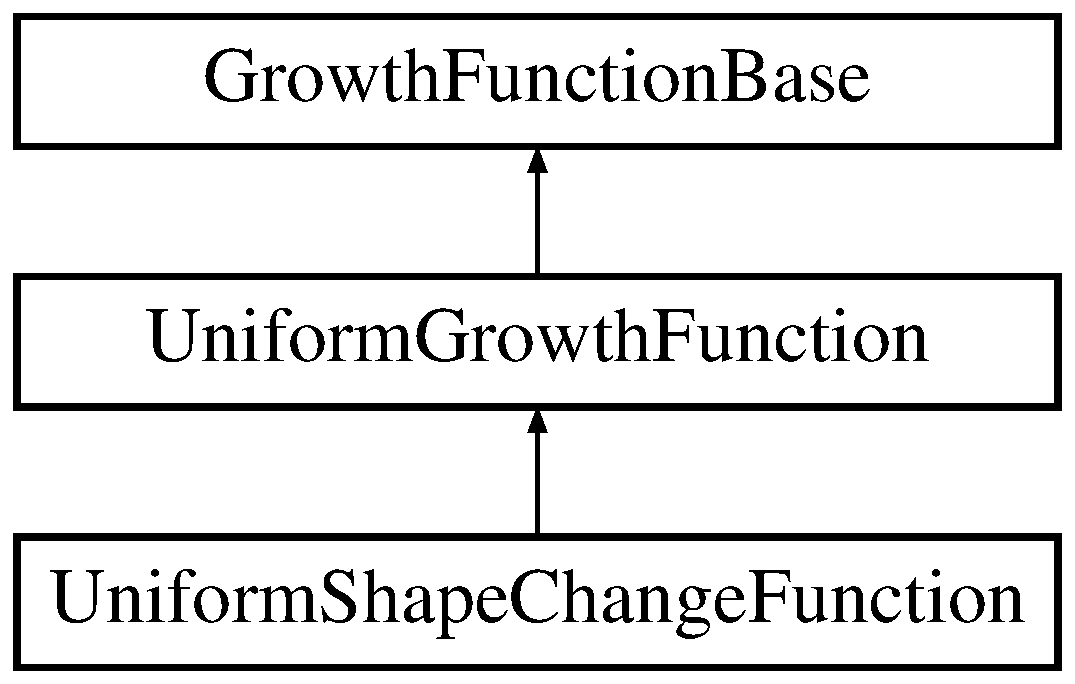
\includegraphics[height=3.000000cm]{classUniformGrowthFunction}
\end{center}
\end{figure}
\subsection*{Public Member Functions}
\begin{DoxyCompactItemize}
\item 
\hyperlink{classUniformGrowthFunction_ab5d7f19747a71d71cec5cc6d55b93a36}{Uniform\+Growth\+Function} (int id, int type, float \hyperlink{classGrowthFunctionBase_ae92513a7b41637df8e26e7db35ddf97c}{init\+Time}, float \hyperlink{classGrowthFunctionBase_a3ff4db0573d354a75666a5f3ca446941}{end\+Time}, bool \hyperlink{classGrowthFunctionBase_a3d56771e7c145589a14e11cc331e0326}{apply\+To\+Columnar\+Layer}, bool \hyperlink{classGrowthFunctionBase_a08ae19f58cb98fa8e315a77f52749732}{apply\+To\+Peripodial\+Membrane}, double D\+V\+Growth, double A\+P\+Growth, double A\+B\+Growth, double \hyperlink{classUniformGrowthFunction_a1a985ff52f9796688e00942b4d3349f8}{angle})
\begin{DoxyCompactList}\small\item\em The constructor of \hyperlink{classUniformGrowthFunction}{Uniform\+Growth\+Function}. \end{DoxyCompactList}\item 
void \hyperlink{classUniformGrowthFunction_ad5be18ae004a3eed205ab3570e13202a}{get\+Growth\+Rate} (double $\ast$max\+Values)
\begin{DoxyCompactList}\small\item\em The function is to get the 3\+D growth rate of the current growth function. \end{DoxyCompactList}\item 
void \hyperlink{classUniformGrowthFunction_aff899907569af697d47927f61b6871a5}{set\+Growt\+Rate} (double ex, double ey, double ez)
\begin{DoxyCompactList}\small\item\em The function is to set the 3\+D growth rate of the current growth function. \end{DoxyCompactList}\item 
\hypertarget{classUniformGrowthFunction_a5a7e9b102a299b94ba648513b66f9cd1}{}gsl\+\_\+matrix $\ast$ \hyperlink{classUniformGrowthFunction_a5a7e9b102a299b94ba648513b66f9cd1}{get\+Shear\+Angle\+Rotation\+Matrix} ()\label{classUniformGrowthFunction_a5a7e9b102a299b94ba648513b66f9cd1}

\begin{DoxyCompactList}\small\item\em The function return the matrix pointer to the oriented growth rotation matrix. \end{DoxyCompactList}\item 
\hypertarget{classUniformGrowthFunction_a8a60d83743c441f7453af8053d5e7010}{}double \hyperlink{classUniformGrowthFunction_a8a60d83743c441f7453af8053d5e7010}{get\+Shear\+Angle} ()\label{classUniformGrowthFunction_a8a60d83743c441f7453af8053d5e7010}

\begin{DoxyCompactList}\small\item\em The function returns the oriented growth angle in radians (double). \end{DoxyCompactList}\item 
void \hyperlink{classUniformGrowthFunction_a227ffb3a524779628f98f110d3811399}{write\+Summary} (ofstream \&save\+File\+Simulation\+Summary, double dt)
\begin{DoxyCompactList}\small\item\em The function is to write the growth function summary to simulation summary file. \end{DoxyCompactList}\end{DoxyCompactItemize}
\subsection*{Public Attributes}
\begin{DoxyCompactItemize}
\item 
\hypertarget{classUniformGrowthFunction_af78591902b0cc391a62f3093fd14ad10}{}double \hyperlink{classUniformGrowthFunction_af78591902b0cc391a62f3093fd14ad10}{Growth\+Rate} \mbox{[}3\mbox{]}\label{classUniformGrowthFunction_af78591902b0cc391a62f3093fd14ad10}

\begin{DoxyCompactList}\small\item\em The double array stating the uniform growth rate throughout the tissue. Growth rate is in 1/sec, format\+: \mbox{[} D\+V axis (x), A\+P axis (y), and A\+B axis (z)\mbox{]}. \end{DoxyCompactList}\item 
\hypertarget{classUniformGrowthFunction_afef9ac84dfe60bbf3d558fbb31946087}{}gsl\+\_\+matrix $\ast$ \hyperlink{classUniformGrowthFunction_afef9ac84dfe60bbf3d558fbb31946087}{Shear\+Angle\+Rotation\+Matrix}\label{classUniformGrowthFunction_afef9ac84dfe60bbf3d558fbb31946087}

\begin{DoxyCompactList}\small\item\em The rotation matrix for the orientation of the growth on x-\/y plane. This matrix is constructed through \hyperlink{classUniformGrowthFunction_a1a985ff52f9796688e00942b4d3349f8}{Uniform\+Growth\+Function\+::angle}. \end{DoxyCompactList}\item 
\hypertarget{classUniformGrowthFunction_a1a985ff52f9796688e00942b4d3349f8}{}double \hyperlink{classUniformGrowthFunction_a1a985ff52f9796688e00942b4d3349f8}{angle}\label{classUniformGrowthFunction_a1a985ff52f9796688e00942b4d3349f8}

\begin{DoxyCompactList}\small\item\em The rotation angle for the orientation of the growth on x-\/y plane. \end{DoxyCompactList}\end{DoxyCompactItemize}


\subsection{Constructor \& Destructor Documentation}
\hypertarget{classUniformGrowthFunction_ab5d7f19747a71d71cec5cc6d55b93a36}{}\index{Uniform\+Growth\+Function@{Uniform\+Growth\+Function}!Uniform\+Growth\+Function@{Uniform\+Growth\+Function}}
\index{Uniform\+Growth\+Function@{Uniform\+Growth\+Function}!Uniform\+Growth\+Function@{Uniform\+Growth\+Function}}
\subsubsection[{Uniform\+Growth\+Function}]{\setlength{\rightskip}{0pt plus 5cm}Uniform\+Growth\+Function\+::\+Uniform\+Growth\+Function (
\begin{DoxyParamCaption}
\item[{int}]{id, }
\item[{int}]{type, }
\item[{float}]{init\+Time, }
\item[{float}]{end\+Time, }
\item[{bool}]{apply\+To\+Columnar\+Layer, }
\item[{bool}]{apply\+To\+Peripodial\+Membrane, }
\item[{double}]{D\+V\+Growth, }
\item[{double}]{A\+P\+Growth, }
\item[{double}]{A\+B\+Growth, }
\item[{double}]{angle}
\end{DoxyParamCaption}
)\hspace{0.3cm}{\ttfamily [inline]}}\label{classUniformGrowthFunction_ab5d7f19747a71d71cec5cc6d55b93a36}


The constructor of \hyperlink{classUniformGrowthFunction}{Uniform\+Growth\+Function}. 

The first six parameters will be directed to the parent constructor, \hyperlink{classGrowthFunctionBase_a061b31ad8a0cb228628c7104029a94bf}{Growth\+Function\+Base\+::\+Growth\+Function\+Base}. ~\newline
doubles D\+V\+Growth, A\+P\+Growth and A\+B\+Growth will set the \hyperlink{classUniformGrowthFunction_af78591902b0cc391a62f3093fd14ad10}{Uniform\+Growth\+Function\+::\+Growth\+Rate}, in the given order.

\subsection{Member Function Documentation}
\hypertarget{classUniformGrowthFunction_ad5be18ae004a3eed205ab3570e13202a}{}\index{Uniform\+Growth\+Function@{Uniform\+Growth\+Function}!get\+Growth\+Rate@{get\+Growth\+Rate}}
\index{get\+Growth\+Rate@{get\+Growth\+Rate}!Uniform\+Growth\+Function@{Uniform\+Growth\+Function}}
\subsubsection[{get\+Growth\+Rate}]{\setlength{\rightskip}{0pt plus 5cm}void Uniform\+Growth\+Function\+::get\+Growth\+Rate (
\begin{DoxyParamCaption}
\item[{double $\ast$}]{max\+Values}
\end{DoxyParamCaption}
)\hspace{0.3cm}{\ttfamily [inline]}, {\ttfamily [virtual]}}\label{classUniformGrowthFunction_ad5be18ae004a3eed205ab3570e13202a}


The function is to get the 3\+D growth rate of the current growth function. 

This function will write the \hyperlink{classUniformGrowthFunction_af78591902b0cc391a62f3093fd14ad10}{Uniform\+Growth\+Function\+::\+Growth\+Rate} of the current growth function to the input double array pointer. The double array pointer should be set to point at a double array of size 3 (or higher) before calling the fucntion.

Reimplemented from \hyperlink{classGrowthFunctionBase}{Growth\+Function\+Base}.

\hypertarget{classUniformGrowthFunction_aff899907569af697d47927f61b6871a5}{}\index{Uniform\+Growth\+Function@{Uniform\+Growth\+Function}!set\+Growt\+Rate@{set\+Growt\+Rate}}
\index{set\+Growt\+Rate@{set\+Growt\+Rate}!Uniform\+Growth\+Function@{Uniform\+Growth\+Function}}
\subsubsection[{set\+Growt\+Rate}]{\setlength{\rightskip}{0pt plus 5cm}void Uniform\+Growth\+Function\+::set\+Growt\+Rate (
\begin{DoxyParamCaption}
\item[{double}]{ex, }
\item[{double}]{ey, }
\item[{double}]{ez}
\end{DoxyParamCaption}
)\hspace{0.3cm}{\ttfamily [inline]}, {\ttfamily [virtual]}}\label{classUniformGrowthFunction_aff899907569af697d47927f61b6871a5}


The function is to set the 3\+D growth rate of the current growth function. 

This function will set the \hyperlink{classUniformGrowthFunction_af78591902b0cc391a62f3093fd14ad10}{Uniform\+Growth\+Function\+::\+Growth\+Rate} of the current growth function to the input values The parameters are in the order \mbox{[} D\+V axis (x), A\+P axis (y), and A\+B axis (z)\mbox{]}.

Reimplemented from \hyperlink{classGrowthFunctionBase}{Growth\+Function\+Base}.

\hypertarget{classUniformGrowthFunction_a227ffb3a524779628f98f110d3811399}{}\index{Uniform\+Growth\+Function@{Uniform\+Growth\+Function}!write\+Summary@{write\+Summary}}
\index{write\+Summary@{write\+Summary}!Uniform\+Growth\+Function@{Uniform\+Growth\+Function}}
\subsubsection[{write\+Summary}]{\setlength{\rightskip}{0pt plus 5cm}void Uniform\+Growth\+Function\+::write\+Summary (
\begin{DoxyParamCaption}
\item[{ofstream \&}]{save\+File\+Simulation\+Summary, }
\item[{double}]{dt}
\end{DoxyParamCaption}
)\hspace{0.3cm}{\ttfamily [inline]}, {\ttfamily [virtual]}}\label{classUniformGrowthFunction_a227ffb3a524779628f98f110d3811399}


The function is to write the growth function summary to simulation summary file. 

This function will write the \hyperlink{classUniformGrowthFunction}{Uniform\+Growth\+Function} details into the simulation summary file, provided as the first input. Time step (dt) of the simulation is provided as second input, to report the growth rates per hour. The output should look like\+: ~\newline
 Growth Type\+: Uniform (1) Initial time(sec)\+: \hyperlink{classGrowthFunctionBase_ae92513a7b41637df8e26e7db35ddf97c}{Uniform\+Growth\+Function\+::init\+Time} Final\+Time time(sec)\+: \hyperlink{classGrowthFunctionBase_a3ff4db0573d354a75666a5f3ca446941}{Uniform\+Growth\+Function\+::end\+Time} Growth\+Rate(fraction/hr)\+: D\+V\+Growth(in 1/hr) A\+P\+Growth(in 1/hr) A\+B\+Growth(in 1/hr)

Reimplemented from \hyperlink{classGrowthFunctionBase}{Growth\+Function\+Base}.



Reimplemented in \hyperlink{classUniformShapeChangeFunction_a196a7555899800406ee62714a20b34c4}{Uniform\+Shape\+Change\+Function}.



The documentation for this class was generated from the following file\+:\begin{DoxyCompactItemize}
\item 
/home/melda/\+Documents/\+Tissue\+Folding/\+Tissue\+Folding/\+Source\+Code/Growth\+Function\+Types.\+h\end{DoxyCompactItemize}

\hypertarget{classUniformShapeChangeFunction}{}\section{Uniform\+Shape\+Change\+Function Class Reference}
\label{classUniformShapeChangeFunction}\index{Uniform\+Shape\+Change\+Function@{Uniform\+Shape\+Change\+Function}}
Inheritance diagram for Uniform\+Shape\+Change\+Function\+:\begin{figure}[H]
\begin{center}
\leavevmode
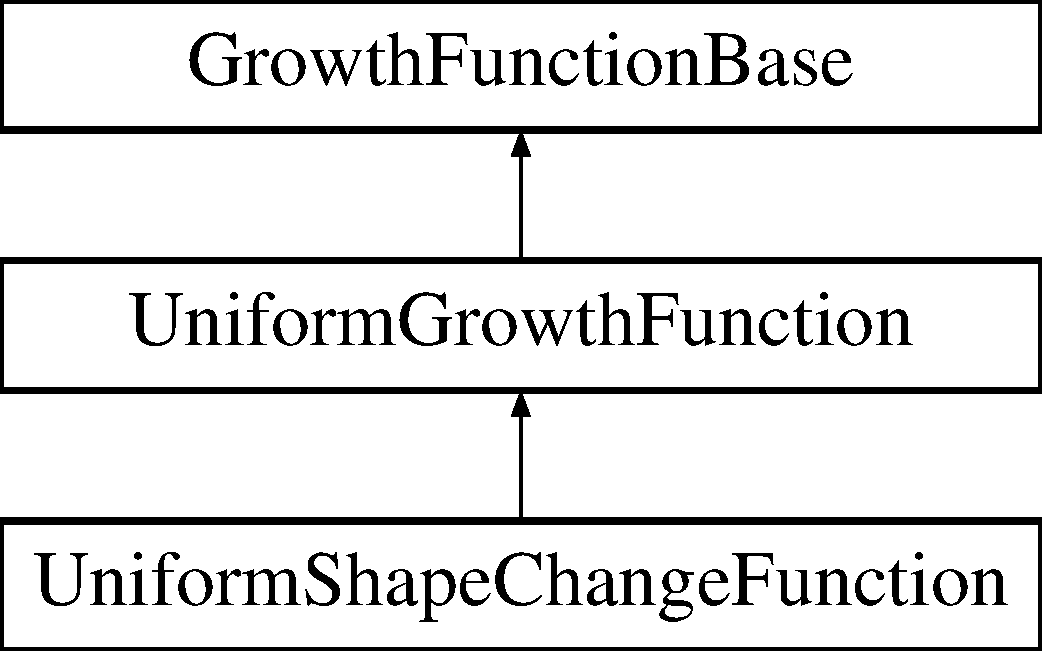
\includegraphics[height=3.000000cm]{classUniformShapeChangeFunction}
\end{center}
\end{figure}
\subsection*{Public Member Functions}
\begin{DoxyCompactItemize}
\item 
\hyperlink{classUniformShapeChangeFunction_a5c4c1a853ab2623416469d3e8b37245a}{Uniform\+Shape\+Change\+Function} (int id, int type, float \hyperlink{classGrowthFunctionBase_ae92513a7b41637df8e26e7db35ddf97c}{init\+Time}, float \hyperlink{classGrowthFunctionBase_a3ff4db0573d354a75666a5f3ca446941}{end\+Time}, bool \hyperlink{classGrowthFunctionBase_a3d56771e7c145589a14e11cc331e0326}{apply\+To\+Columnar\+Layer}, bool \hyperlink{classGrowthFunctionBase_a08ae19f58cb98fa8e315a77f52749732}{apply\+To\+Peripodial\+Membrane}, int Shape\+Change\+Type, double Shape\+Change\+Rate)
\begin{DoxyCompactList}\small\item\em The constructor of \hyperlink{classUniformShapeChangeFunction}{Uniform\+Shape\+Change\+Function}. \end{DoxyCompactList}\item 
void \hyperlink{classUniformShapeChangeFunction_a196a7555899800406ee62714a20b34c4}{write\+Summary} (ofstream \&save\+File\+Simulation\+Summary, double dt)
\begin{DoxyCompactList}\small\item\em The function is to write the growth function summary to simulation summary file. \end{DoxyCompactList}\end{DoxyCompactItemize}
\subsection*{Public Attributes}
\begin{DoxyCompactItemize}
\item 
\hypertarget{classUniformShapeChangeFunction_ac157bf953d6a8e3006988e8913866524}{}int {\bfseries Shape\+Change\+Type}\label{classUniformShapeChangeFunction_ac157bf953d6a8e3006988e8913866524}

\end{DoxyCompactItemize}


\subsection{Constructor \& Destructor Documentation}
\hypertarget{classUniformShapeChangeFunction_a5c4c1a853ab2623416469d3e8b37245a}{}\index{Uniform\+Shape\+Change\+Function@{Uniform\+Shape\+Change\+Function}!Uniform\+Shape\+Change\+Function@{Uniform\+Shape\+Change\+Function}}
\index{Uniform\+Shape\+Change\+Function@{Uniform\+Shape\+Change\+Function}!Uniform\+Shape\+Change\+Function@{Uniform\+Shape\+Change\+Function}}
\subsubsection[{Uniform\+Shape\+Change\+Function}]{\setlength{\rightskip}{0pt plus 5cm}Uniform\+Shape\+Change\+Function\+::\+Uniform\+Shape\+Change\+Function (
\begin{DoxyParamCaption}
\item[{int}]{id, }
\item[{int}]{type, }
\item[{float}]{init\+Time, }
\item[{float}]{end\+Time, }
\item[{bool}]{apply\+To\+Columnar\+Layer, }
\item[{bool}]{apply\+To\+Peripodial\+Membrane, }
\item[{int}]{Shape\+Change\+Type, }
\item[{double}]{Shape\+Change\+Rate}
\end{DoxyParamCaption}
)\hspace{0.3cm}{\ttfamily [inline]}}\label{classUniformShapeChangeFunction_a5c4c1a853ab2623416469d3e8b37245a}


The constructor of \hyperlink{classUniformShapeChangeFunction}{Uniform\+Shape\+Change\+Function}. 

Forst six parameters will be directed to the parent constructor, \hyperlink{classUniformGrowthFunction_ab5d7f19747a71d71cec5cc6d55b93a36}{Uniform\+Growth\+Function\+::\+Uniform\+Growth\+Function}. The growth rates in Dv, A\+B and A\+P will be fed as 0 to the parent constructor. ~\newline
The parameter Shape\+Change\+Type will define the type of the shape change as 1\+: Columnar\+To\+Squamous change, 2\+: Apical shrinkage, and 2\+: basal shrinkage. The paremeter Shape\+Change\+Rate will define the rate of defined shape change. The constructor will calculate the corrected rate, as to conserve the volume while shape change is occuring.

\subsection{Member Function Documentation}
\hypertarget{classUniformShapeChangeFunction_a196a7555899800406ee62714a20b34c4}{}\index{Uniform\+Shape\+Change\+Function@{Uniform\+Shape\+Change\+Function}!write\+Summary@{write\+Summary}}
\index{write\+Summary@{write\+Summary}!Uniform\+Shape\+Change\+Function@{Uniform\+Shape\+Change\+Function}}
\subsubsection[{write\+Summary}]{\setlength{\rightskip}{0pt plus 5cm}void Uniform\+Shape\+Change\+Function\+::write\+Summary (
\begin{DoxyParamCaption}
\item[{ofstream \&}]{save\+File\+Simulation\+Summary, }
\item[{double}]{dt}
\end{DoxyParamCaption}
)\hspace{0.3cm}{\ttfamily [inline]}, {\ttfamily [virtual]}}\label{classUniformShapeChangeFunction_a196a7555899800406ee62714a20b34c4}


The function is to write the growth function summary to simulation summary file. 

This function will write the \hyperlink{classUniformGrowthFunction}{Uniform\+Growth\+Function} details into the simulation summary file, provided as the first input. Time step (dt) of the simulation is provided as second input, to report the growth rates per hour. The output should look like\+: ~\newline
 Growth Type\+: Uniform (1) Initial time(sec)\+: \hyperlink{classGrowthFunctionBase_ae92513a7b41637df8e26e7db35ddf97c}{Uniform\+Growth\+Function\+::init\+Time} Final\+Time time(sec)\+: \hyperlink{classGrowthFunctionBase_a3ff4db0573d354a75666a5f3ca446941}{Uniform\+Growth\+Function\+::end\+Time} Growth\+Rate(fraction/hr)\+: D\+V\+Growth(in 1/hr) A\+P\+Growth(in 1/hr) A\+B\+Growth(in 1/hr)

Reimplemented from \hyperlink{classUniformGrowthFunction_a227ffb3a524779628f98f110d3811399}{Uniform\+Growth\+Function}.



The documentation for this class was generated from the following file\+:\begin{DoxyCompactItemize}
\item 
/home/melda/\+Documents/\+Tissue\+Folding/\+Tissue\+Folding/\+Source\+Code/Growth\+Function\+Types.\+h\end{DoxyCompactItemize}

%--- End generated contents ---

% Index
\backmatter
\newpage
\phantomsection
\clearemptydoublepage
\addcontentsline{toc}{chapter}{Index}
\printindex

\end{document}
